%-------------------------------------------------------------------
% Document class and package definitions
%-------------------------------------------------------------------
\documentclass[12pt,a4paper,openright,final,twoside]{cseethesis}

%Included for Gather Purpose only:
%input "thesisreferences.bib"

% Additional packages for Paper 2
\usepackage{listings}
\usepackage{xcolor}

\makeglossaries

\newacronym{nlp}{NLP}{Natural Language Processing}

\begin{document}

\defaultbibliography{thesisreferences,MX_Papers/Paper2/INDIN2021,MX_Papers/Paper3/refrencias_sobraep}     %% Change this only.
\defaultbibliographystyle{plain}        %% Could be changed if you like 
                                           %% references typeset differently.
%-------------------------------------------------------------------
% Define title, author, etc.
%-------------------------------------------------------------------
\def\thesistitle{Example Thesis updated by Tosin Adewumi}

\begin{figure}[h]
 \centering
 
\includegraphics[width=0.5\textwidth]{bg_wall.jpg}
\end{figure}

\def\theauthor{Johan E.\ Carlson}
\def\theaddress{Dept.\ of Computer Science, Electrical and Space Engineering\\
Lule{\aa} University of Technology\\ Lule{\aa}, Sweden}

\def\supervisors{Name of your supervisor(s)}
\def\supervisorstring{Supervisors:} % Edit here if you have only one supervisor
\def\dedication{To my surprise...}

% Read abstract and preface from separate files.
% Make sure these exist. See example files.
\def\theabstract{IEC 61499 is a standard for modular and event-driven industrial automation, enabling distributed control through function blocks (FBs). This architecture enhances reusability, interoperability, and scalability, making it well-suited for cyber-physical automation systems. One of the major challenges in this context is balancing dependability with flexibility. As systems evolve, rapid revalidation becomes essential. Automatic testing plays a crucial role in addressing this by enabling quick verification after changes. However, when deploying this architecture in safety-critical systems, automatic testing alone is insufficient. To ensure correctness and reliability, formal verification techniques are required. Closed-loop verification helps mitigate state-space explosion by integrating plant models with the control logic, allowing for more rigorous analysis. Another key challenge lies in obtaining appropriate models of the physical plant for verification. One practical solution is to leverage existing simulation models, discretize them, and inject non-determinism to represent execution uncertainties. Process mining techniques facilitate the construction of plant models by analyzing event logs from digital twins, providing an accurate representation of system behavior. This approach ensures robust validation, verifying system performance under diverse conditions and operational uncertainties. 

IEC 61499 provides a modular framework for designing control systems, enabling reconfigurable and flexible manufacturing. Blockchain-based traceability enhances security and ensures verification in flexible production system. AI-driven automation further optimizes industrial control by enabling intelligent decision-making, real-time adjustments, and process adaptation. AI agents, leveraging large language models (LLMs) and knowledge graphs (KGs), enhance human-machine collaboration by analyzing tasks and executing actions via OPC UA. These agents can interpret operator instructions, generate and validate execution sequences, and ensure conformance with specified requirements to support reliable and adaptive industrial automation.}
\def\thepreface{The creation of this template has taken several years, and the shape it is in now would not have been possible with out the patient testers out there. To mention just a few who found and reported bugs, and occasionally even provided bug fixes: Gustav Johansson, Sara Sandberg, Yvonne Aitomäki, Fredrik Hägglund, Jesper Martinsson, Patrik Pääjärvi, and Martin Sehlstedt. To all of those I forgot to mention, please accept my apologies.\\[2.5cm]
Luleå, June 2009\\
Johan E.\ Carlson \\ \\
Improvements by Tosin Adewumi, October 9, 2021.}


% Change here if you want to remove the logo printed on the first page

%\def\thelogo{
\includegraphics[width=2.5cm]{bg_wall.jpg}} % old EU logo
\def\thelogo{} % no logo

% The definitions above could be put directly in the function call below,
% but is here defined explicitly, for the purpose of clarity.

\startpreamble
  {\thesistitle}
  {\theauthor}
  {\theaddress}
  {\supervisors}
  {\dedication}
  {\theabstract}
  {\thepreface}
  {\thelogo}

%%%%%%%%%%%%%%%%%%%%%%%%%%%%%%%%%%%%%%%%%%%%%%%%%%%%%%%%%%%%%%%%%%%%
%% Begin Part I
%%%%%%%%%%%%%%%%%%%%%%%%%%%%%%%%%%%%%%%%%%%%%%%%%%%%%%%%%%%%%%%%%%%%
\makepartpage{Part I} 

%% Initialize part containing the thesis introduction chapters
\startchapters
\begin{bibunit}
%------------------------ Start chapter 1 --------------------------
% The \makechapter command takes three arguments
%  1) An abbreviated version of the chapter name,
%     to be used as page header
%  2) String to be added to the table of contents
%  3) The chapter name, possibly split in to lines,
%     as in Chapter 2 below.
%
%  The different arguments can have different line breaks.
%
% The actual contents of the chapter is included by removing the
% comment from the \input line below. Make sure the file
% chapter1.tex exists.
%-------------------------------------------------------------------

\def\myquote{``This report, by its very length, defends itself against the risk of being read."\\[.5\baselineskip] Winston Churchill}

\makechapter[\myquote]{Thesis Introduction}{Thesis Introduction}{Thesis
Introduction\label{ch1}}
\section{General information}
Current version of the \texttt{cseethesis} document class is: \classversion.\\
Last modification: \classdate\\

\noindent As of version 3.0, the template is no longer backwards compatible.

\subsection{About the document class}
This document class was originally created in 2002 when I was working on my own PhD thesis. Since then, many people used it, found bugs (and occasionally even corrected them), and suggested improvements.

The style is tailor-made for the typical types of theses that we write at the department, i.e.\ an introductory part followed by a collection of published or submitted research papers. 

The template supports the use of both \LaTeX\ and pdfLaTeX. If you use the command \texttt{$\backslash$includegraphics} to import your figure and you supply the filename with its extension (e.g.\ .eps, .pdf), compilation should be possible with either one. For this to work, both .eps and .pdf versions of all figures must be available.

The template is totally free to use, modify and distribute, as long as reference to the original author is kept and as long as all files remain in the package. Modified versions can only be distributed if it is clearly mentioned in the document class that modifications have been made and by whom.

The whole package comes AS IS. I will correct bugs every now and then, but other than that, don't expect any support whatsoever.


\subsection{About this document}
This document, as well as the actual \LaTeX\ code for it, makes up the documentation on how to use the document class.

Only this chapter contains any readable information. Chapters 2 and 3 are only included as examples of some of the features of the template. The text is nonsense, but the corresponding \LaTeX\ code may be of some use. The same goes for the appended papers, which are only there as examples of a few options of the document class.

Read this chapter carefully. If you have comments on what else should be in here in order to simplify the use of the document class, let me know.

\section{Chapters}
\subsection{Defining chapters}
In order to add flexibility to the template, a new command, called \texttt{$\backslash$makechapter} is provided. This command takes three mandatory and one optional argument, as 
\begin{center}
	\texttt{$\backslash$makechapter[optional quote]\{page header\}\{toc entry\}\{Chapter title\}}
\end{center}

The reason this is solved like this is to allow for shorter page headers if the chapter name is very long. Also, if the actual chapter heading needs to be manually split in several lines (if the automatic splitting does not look so good), the table of contents (toc) entry might have to be defined differently. Note that normally, the last three arguments can be the same. 

The use of an optional quote as an introduction to the chapter is demonstrated in this chapter. It can just as well be left out, which is demonstrated in this document (see the code).

\subsection{Importing chapter contents}
The sub-documents containing the chapters should start directly, i.e.\ they must not contain any $\backslash$begin\{document\} or $\backslash$end\{document\} tags.

See this file, \textit{chapter1.tex} for details.

\section{How to append papers}
Papers are included using the \texttt{$\backslash$input} command, just as with chapters. You have to typeset paper title, authors, and abstract manually. See the example papers accompanying this document for an example.

To make the separator sheet preceding each paper, use one of the following commands:
\begin{itemize}
	\item \texttt{$\backslash$makepaper} -- Published paper.
	\item \texttt{$\backslash$makepaperaccepted} -- Accepted, not yet published paper.
	\item \texttt{$\backslash$makepapersubmitted} -- Submitted, not yet accepted paper.
	\item \texttt{$\backslash$makepapertobesubmitted} -- Not yet submitted paper.
\end{itemize}

See code for this example document for examples on how to use.

\section{Cross-references}
All labels throughout the thesis have to be unique. If the same
equation or figure shows up twice e.g.\ a figure used
both in the introduction and one of the included papers), it has
to be given different labels. Referring to labels is done as
usual.

A simple trick to make sure this is the case and that will also help you keep track of all labels you used is to use the following naming convention:
\begin{itemize}
	\item \texttt{ch1:fig:labelname}, \texttt{ch1:tab:labelname}, \texttt{ch1:eq:labelname}, etc.\ all denote figures, tables and equations in Chapter 1.
	\item \texttt{paperA:fig:labelname}, \texttt{paperA:tab:labelname}, \texttt{paperA:eq:labelname}, etc.\ all denote figures, tables and equations in Paper A.
\end{itemize}

For existing text, e.g.\ papers, this is easily achieved by a simple search-and-replace operation on the string \texttt{$\backslash$label\{}. Any text editor will do that for you!

\section{Appendices\label{sec:app}}
It is possible to have any number of appendices for each chapter.
Simply type \texttt{$\backslash$appendix} before the first appendix,
which is then a normal \texttt{section}, but numbered differently.

To add appendices to papers, use the
\texttt{$\backslash$paperappendix} command

\section{Including bibliography lists\label{sec:bib}}
In a thesis one might want several separate bibliographies. For
example, one for the first part, and then separate bibliographies
for each of the included papers.

This is solved using the \texttt{bibunits} package together with a
slight work-around in this template. For the first part of the
thesis, there is only one bibliography list, typeset like a chapter
(see this example document). In the papers, the bibliography lists
are typeset as un-numbered sections. See this file
\texttt{cseethesis\_example.tex} and \texttt{paper1.tex} for examples
how to place the bibliographies. 

Note that the command
\begin{itemize}
	\item \texttt{$\backslash$makebib} is used in Part I, to typeset the reference list in the thesis introduction.
	\item \texttt{$\backslash$putbib} is used in the papers in Part II.
\end{itemize}

\section{How to compile your project}
Finally, you probably like to know how to build your project to a
final PDF or PostScript file. Start by verifying that you can
compile this document. This is how it goes:
%
\begin{enumerate}
    \item Run \LaTeX\ (or pdfLaTex) once.
    \item Then run BibTeX on all the
    bu<i> files.
    \item Run \LaTeX\ twice more, to build the final DVI document
    (or pdfLaTeX if you want a PDF file).
\end{enumerate}

The above steps are easily collected in a script or batch file. See
the files \texttt{make.bat} and \texttt{compilebibunits.bat} for
examples.

\section{Revision history}
The template has evolved during several years and the exact
revisions are not clear to anyone. Starting from version 1.6,
however, the changes are more well-documented. This example
document will always support only the latest release of the
template. Below is a list of the revisions made to the document
class (and when applicable, the example document):%
\begin{itemize}
	 \item Version 3.1, September 1, 2010
		\begin{itemize}
			\item Fixed bug related to appendix numbering.
			\item Fixed page numbering of ``Part" pages.
			\item Added a comment at top of cseethesis\_example.tex, for improved compatibility with some editors.
		\end{itemize}
	 \item Version 3.0, June 7, 2009
		\begin{itemize}
			\item Fixed bug related to page headers in chapters containing no subsections.
		   \item Removed the EU class option and replaced with a logo argument to the preamble. See the code of this document for an example.
			\item The template is \textbf{no longer compatible with previous versions}.
         \item Removed the definition of boldface Greek letters from the document class, since this is not the proper place for that.
		\end{itemize}
  	 \item Version 2.5, March 5 2009
		\begin{itemize}
         \item Renamed the template \textit{cseethesis}. It is a continuation of the project initially called \textit{eisthesis}, but since its use has spread I decided to change the name.
			\item Various minor bug fixes.
			\item Update of example document, making examples of additions and revisions in recent versions of the template.
		\end{itemize}
	 \item Version 2.36: Added "Part" to the table of contents.
    \item Version 2.35:
        \begin{itemize}
				\item Fixed a bug regarding the page headers in the "appended papers part".
				\item Fixed a bug causing the section numbering to be wrong in a chapter succeeding a chapter containing appendices.
			   \item Added a chapter 3 in this example document, illustrating how to handle page headers for chapters without any sections. See the code at the top of \texttt{chapter3.tex}.
		  \end{itemize}
    \item Version 2.3:
        \begin{itemize}
            \item Added the commands \texttt{$\backslash$appendix}
            and \texttt{$\backslash$paperappendix}, see section
            \ref{sec:app}.
            \item The bibliography list is now typeset similar to a
            chapter in Part I, and as an un-numbered section in Part
            II. This required the use of separate commands for
            including the lists (see Sec.~\ref{sec:bib})
            \item Typesetting fixes for the table of contents page.
            As a consequence, the package \texttt{titletoc} is now
            required.
            \item Minor other code cleanup and bug fixes.
        \end{itemize}
    \item Version 2.25:
    \begin{itemize}
        \item Fixed a minor bug that used to generate a warning
        message regarding font shapes in the page headers.
    \end{itemize}
    \item Version 2.2:
    \begin{itemize}
        \item pdf and eps class options removed. The document class
        compiles with either pdfLaTeX or \LaTeX.
        \item The reference lists in papers are now typeset in the
        same way as in Part I of the thesis.
        \item Some minor adjustments of page header heights.
    \end{itemize}
    \item Version 2.1:
    \begin{itemize}
        \item Cross-references to chapters now work like they
        should. See the main document of this example.
        \item Major bug fixes to BibTeX reference lists, table of
        contents generation etc.
        \item The only change the user has to do is to use the new \texttt{$\backslash$makebib} instead of
        bibunits' \texttt{$\backslash$putbib}.
    \end{itemize}
    \item Version 2.0:
    \begin{itemize}
        \item Support for EU logotype on main page. The files
        \texttt{eu1\_f\_eng.pdf} and\\ \texttt{eu1\_f\_eng.eps} must be
        placed in the same directory as the document class.
        \item Support for pdf class options.
        \item Update of the \texttt{$\backslash$makechapter}
        command. It now requires three arguments. See main
        document for example.
        \item Support for BibTeX, using the \texttt{bibunits.sty}
        package.
    \end{itemize}
    \item Version 1.6: Various bug fixes to figure spacing etc.
\end{itemize}


\makechapter{Running header}{Table of contents entry}{Title
appearing on the\\ chapter start page\label{ch2}}
\section{Introduction}

Industrial automation is undergoing a significant transformation, driven by the need for mass customization, increased flexibility, and reconfigurability. This has led to the adoption of modular, distributed architectures, often termed Component-Based industrial Automation Systems (CBAS) or, more broadly, industrial Cyber-Physical Systems (iCPS). The International Electrotechnical Commission (IEC) 61499 standard has emerged as a key enabler for engineering these complex systems, providing a vendor-independent, component-based model for distributed control applications.

However, the increased complexity and distributed nature of these systems pose significant verification and validation (V\&V) challenges. Traditional V\&V techniques, such as simulation and testing, are often inadequate for ensuring the high levels of dependability, safety, and reliability required, particularly in safety-critical domains like nuclear material handling or power grid protection. While simulation is invaluable for assessing general system behavior, it cannot explore the entire state space of complex industrial software, meaning it can show the presence of bugs but not their absence.

To address this gap, formal methods offer a mathematically rigorous approach to system verification. Model checking, in particular, is an automated technique that systematically explores all reachable states of a system model to verify whether it satisfies a given set of formal specifications, typically expressed in temporal logic. Despite its power to uncover subtle design flaws that simulation might miss, the adoption of model checking in industrial practice has been limited. This is often due to challenges such as the state-space explosion problem, the need for specialized expertise to create formal models, and a lack of user-friendly tools that integrate seamlessly into the existing engineering lifecycle.

This chapter presents an integrated, model-based framework designed to bridge this gap. It leverages the IEC 61499 standard not only for controller design but also for modeling the system's environment (the "plant"), creating a comprehensive closed-loop model suitable for rigorous verification. The framework incorporates a seamless toolchain that automates the translation of IEC 61499 designs into a formal representation for a powerful model checker, and provides intuitive tools for analyzing the results. Key contributions of this framework include a novel notation for introducing non-determinism into plant models to make verification more realistic and a specific methodology for verifying the correctness of runtime safety monitors.

The chapter is structured as follows. Section \ref{sec:iec61499} provides an overview of the IEC 61499 standard. Section \ref{sec:formal_verification} introduces the principles of formal verification and the closed-loop modeling paradigm. Section \ref{sec:toolchain} details the components of the integrated toolchain and the associated methodologies for enhancing verification. Section \ref{sec:case_studies} demonstrates the practical application of the framework through several case studies, from laboratory-scale systems to a safety-critical industrial machine. Finally, Section \ref{sec:conclusion} concludes the chapter and discusses future research directions.

\section{The IEC 61499 Standard for Distributed Automation}\label{sec:iec61499}

The IEC 61499 standard provides a reference architecture for the development of distributed control systems. It was conceived as a successor to the prevalent IEC 61131-3 standard, moving beyond the limitations of centralized, PLC-centric logic to support the demands of modern, distributed iCPS.

At the core of the standard is the Function Block (FB), a reusable software component that encapsulates data and algorithms. FBs interact through a well-defined graphical interface consisting of event and data inputs and outputs. The execution of logic within an FB is event-driven; an input event triggers the execution of associated algorithms and may result in the emission of one or more output events, propagating the flow of control through the network.

The standard defines several types of FBs, with the most fundamental being the Basic Function Block (BFB). The internal logic of a BFB is defined by an Execution Control Chart (ECC), which is a state machine that dictates the sequence of algorithm execution in response to input events. A Composite Function Block (CFB), in contrast, contains an internal network of other interconnected FBs, enabling hierarchical system design. This component-based, event-driven nature makes IEC 61499 inherently suited for modeling modular, reconfigurable, and distributed systems.

Despite these advantages, the verification of IEC 61499 applications is a recognized challenge. The concurrent and distributed nature of the systems can lead to complex emergent behaviors that are difficult to predict. Furthermore, ambiguities in the standard's original execution semantics led to different interpretations by tool vendors, creating portability and interoperability issues that formal modeling can help to identify and resolve.

\section{Formal Verification for IEC 61499 Systems}\label{sec:formal_verification}

Formal verification is the process of using mathematical methods to prove or disprove the correctness of a system with respect to a set of formal specifications. Model checking is a prominent formal verification technique that automates this process. It operates on a finite-state model of the system, systematically exploring all possible execution paths to check if they satisfy properties expressed in a formal language, such as Linear Temporal Logic (LTL) or Computation Tree Logic (CTL). If a property is violated, the model checker produces a counterexample—a specific trace of execution that demonstrates the failure.

\subsection{The Closed-Loop Modeling Paradigm}

A crucial aspect of applying model checking effectively to control systems is the adoption of a closed-loop modeling approach. Verifying a controller in isolation (open-loop) requires making assumptions about all possible inputs it might receive from its environment, which often leads to an unmanageably large state space and can produce spurious counterexamples that are not possible in the real system.

A closed-loop model, by contrast, includes a formal model of the plant—the physical process or environment the controller interacts with. This model constrains the inputs to the controller to only those that are physically possible, drastically reducing the reachable state space and leading to more meaningful verification results. This architecture, encompassing both the controller and the plant, allows for the verification of system-level properties that involve interactions between the two.

\begin{figure}[h]
\centering
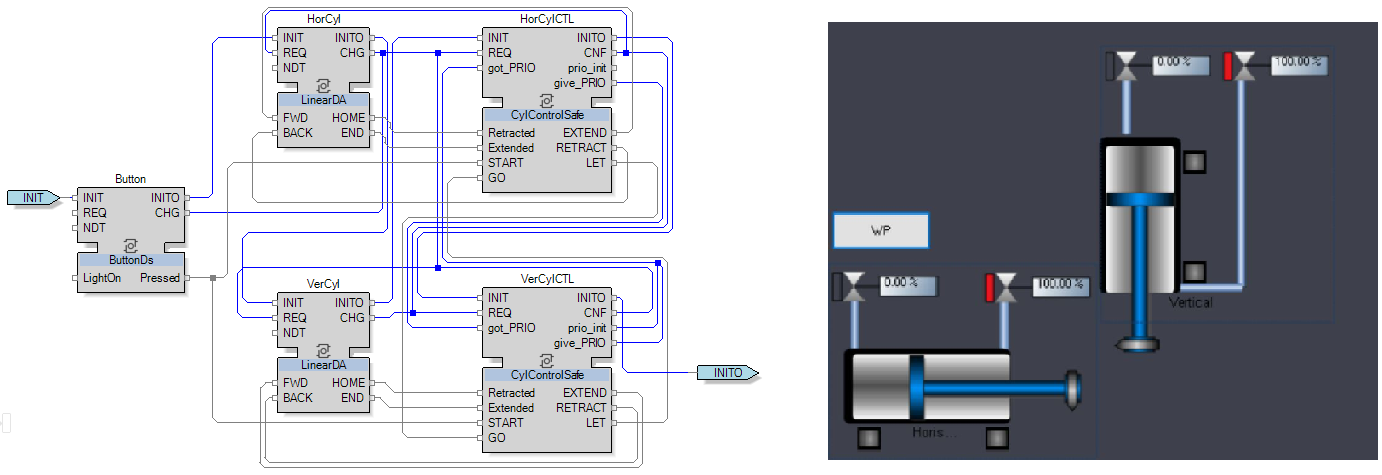
\includegraphics[width=0.8\textwidth]{MX_Papers/Paper3/pic/wholesystem_withhmi.png}
\caption{An illustration of the closed-loop modeling concept, where a controller (or a non-deterministic twin, right) is verified in conjunction with a monitor (left), representing an interconnected system.}
\label{fig:closed_loop}
\end{figure}

\subsection{From Simulation to Verification Models}

The IEC 61499 standard is well-suited for closed-loop modeling because the same component-based language can be used to model both the controller and the plant. This allows for a seamless transition from simulation to formal verification.

Initially, a detailed plant model, often equivalent to a hybrid automaton with continuous dynamics, can be created for simulation-in-the-loop to test the overall system behavior and provide visualization. For formal verification, this detailed model is then abstracted into a simpler, discrete-state model that captures the essential behaviors relevant to the properties being checked, but omits complexities like continuous dynamics that are computationally expensive for model checkers to handle. This dual-model approach allows engineers to use familiar tools for design and simulation, while enabling a pathway to rigorous formal verification.

\section{An Integrated Verification Toolchain and Methodology}\label{sec:toolchain}

To make formal verification practical for automation engineers, a seamless and highly automated toolchain is required. The framework presented here integrates industry-standard design environments with a powerful open-source model checker, facilitated by a custom model generator and advanced analysis tools.

\subsection{Overview of the Toolchain}

The proposed workflow connects the design, verification, and analysis phases into a cohesive process.

\begin{figure}[h]
\centering
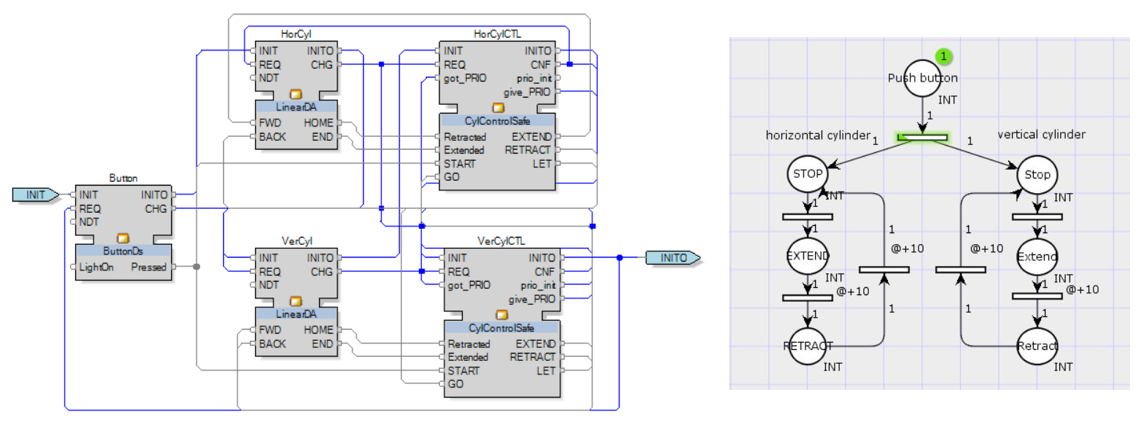
\includegraphics[width=0.9\textwidth]{MX_Papers/Paper3/pic/system_functional_model.png}
\caption{The proposed workflow for the design and validation of safety-critical automation systems, integrating design, simulation, formal model generation, model checking, and counterexample analysis.}
\label{fig:workflow}
\end{figure}

The toolchain consists of the following key components:

\begin{itemize}
\item \textbf{IEC 61499 Design Environment}: The process begins in an IEC 61499-compliant IDE, such as EcoStruxure™ Automation Expert or the open-source Function Blocks Modelling Environment (FBME), where the controller and plant FBs are designed and simulated.

\item \textbf{Formal Model Generator (fb2smv)}: The fb2smv tool automatically translates the IEC 61499 application, described in its standard XML format, into a formal model in the SMV (Symbolic Model Verifier) language. This tool uses Abstract State Machines (ASM) as an intermediate model to handle the translation of the ECCs, algorithms, and network connections.

\item \textbf{Symbolic Model Checker (NuSMV)}: The generated SMV model is fed into NuSMV, an open-source symbolic model checker. NuSMV verifies the model against the specified LTL or CTL properties and, if a violation is found, generates a counterexample trace.

\item \textbf{Counterexample Analysis Environment (FBME)}: Analyzing the raw text output of a model checker can be difficult and unintuitive. Tools like FBME have been enhanced with trace visualization capabilities that import the counterexample from NuSMV and map it back onto the original graphical IEC 61499 model. This allows engineers to step through the failure trace visually, see the state of ECCs and variable values at each step, and use causal analysis to pinpoint the root cause of the error.
\end{itemize}

\subsection{Enhancing Plant Models with Non-Deterministic Transitions (NDT)}

A key challenge in creating abstracted plant models for verification is ensuring they are realistic enough to capture potential failures. A purely deterministic model, where an action takes a fixed amount of time, may fail to uncover timing-related bugs, such as collisions that occur only when one axis moves faster or slower than another.

To address this, this framework introduces a problem-oriented notation for Non-Deterministic Transitions (NDT) directly within the ECC of an IEC 61499 plant model. An NDT represents a transition that can fire at an arbitrary time after it becomes enabled. For example, in a model of a linear axis, an NDT can be used to model the unknown duration of the motion between two points.

\begin{figure}[h]
\centering
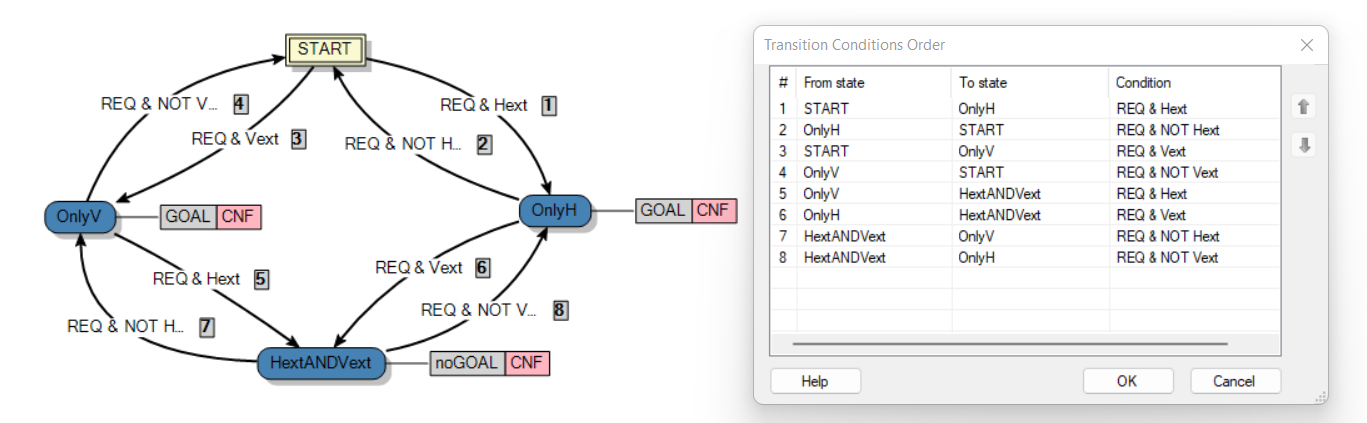
\includegraphics[width=0.7\textwidth]{MX_Papers/Paper3/pic/ECC-moniteur.png}
\caption{An example ECC for an elevator plant model. The transition from the GO state to the END state is triggered by an NDT event, modeling an unspecified amount of time for the motion to complete.}
\label{fig:ecc_ndt}
\end{figure}

When the fb2smv tool encounters an NDT event, it translates it into a non-deterministic choice in the SMV model. This instructs the model checker to explore all possible timings for that transition, effectively simulating a wide range of real-world scenarios (e.g., different relative speeds between concurrent movements) and enabling the detection of subtle, timing-dependent design flaws that would be difficult to find through simulation alone. This ability to govern and selectively inject non-determinism is a powerful feature for performing targeted formal verification under specific stress conditions.

\subsection{A Methodology for Verifying Runtime Monitors}

In addition to offline verification at the design stage, many safety-critical systems utilize online verification through runtime monitors. These monitors, often implemented as FBs themselves, observe the system during operation and signal an error if a safety property is violated. However, a monitor only improves system safety if its own correctness is guaranteed.

Verifying a monitor presents a unique challenge. Traditional open-loop model checking, where the monitor's inputs are allowed to change arbitrarily, will often produce spurious counterexamples. This is because it allows input combinations that are semantically impossible in a real IEC 61499 system, such as data being transferred without a corresponding event firing.

To solve this, a methodology is proposed for the closed-loop model checking of monitors using a non-deterministic twin (ND twin) of the controller it supervises. The ND twin is a simplified FB that abstracts the controller's logic but is designed to produce every possible valid combination of its outputs. It achieves this by using NDTs to allow arbitrary transitions between its key states (e.g., EXTEND, RETRACT, STOP).

By connecting the monitor to this ND twin, the model checker can exhaustively test the monitor's logic against all valid controller behaviors. The verification is then guided by two main properties:

\begin{enumerate}
\item The monitor must report a failure when a failure actually occurs. (e.g., G ((m.hext ∧ m.vext) → (m.hext ∧ m.vext U m.collision)))
\item The monitor must not report a spurious failure when the controller is functioning as expected. (e.g., G (¬(m.hext ∧ m.vext) → F ¬m.collision))
\end{enumerate}

This approach ensures that the monitor is trustworthy before it is deployed for online verification, forming a critical link between offline design-time checks and online runtime safety assurance.

\section{Application to Case Studies}\label{sec:case_studies}

The effectiveness of the proposed framework and methodologies has been demonstrated on several case studies, ranging from laboratory-scale systems to real-world safety-critical applications.

\subsection{System of Two Pneumatic Cylinders}

This system involves two orthogonal pneumatic cylinders that must move without colliding. A runtime monitor, NoCollisionMonitor, was implemented as a BFB to ensure this safety property holds during operation. To verify the monitor, an ND twin of the cylinder controller was created. The ND twin was designed to non-deterministically produce EXTEND, RETRACT, and STOP commands, allowing it to generate the collision scenario (EXTEND from both twins simultaneously) as well as all non-collision scenarios. Using NuSMV, the monitor was successfully verified against the two key properties: it correctly reported the collision when it occurred and did not report false positives, proving its reliability.

\begin{figure}[h]
\centering
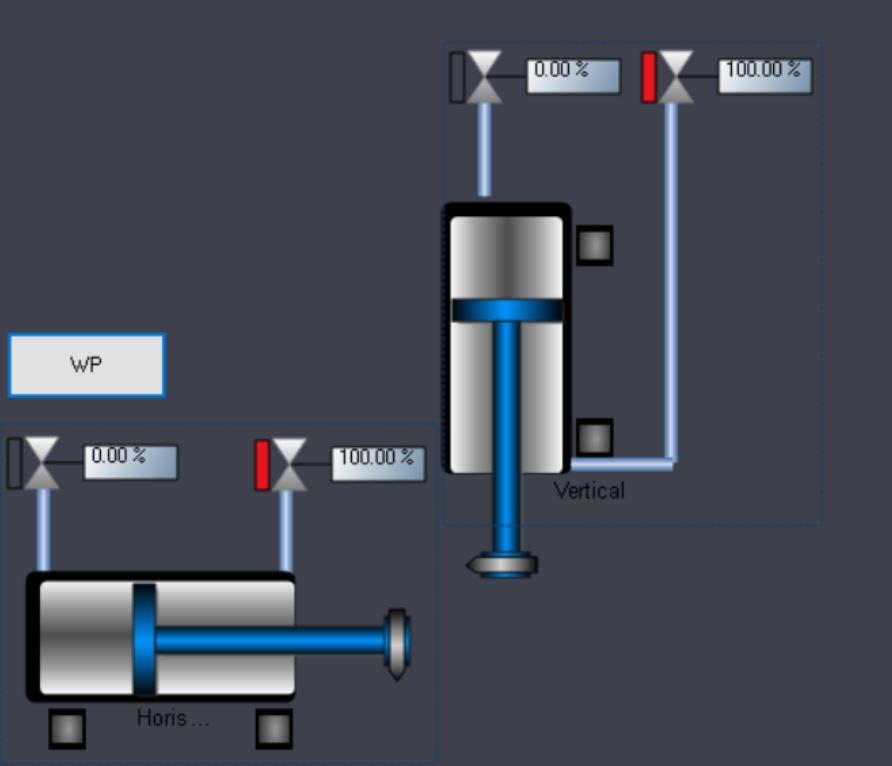
\includegraphics[width=0.8\textwidth]{MX_Papers/Paper3/pic/2cylindre_hmi.JPG}
\caption{The two pneumatic cylinder system with HMI interface, demonstrating the collision detection and prevention mechanism.}
\label{fig:two_cylinders}
\end{figure}

\subsection{Drilling Station}

This case study features a drilling station with a drill and a rotating table. The control logic, implemented in IEC 61499, was designed to prevent the table from rotating while the drill is active. The system was modeled in a closed loop, with NDTs used in the plant models for the drill and table to represent the unknown duration of their movements. During model checking with NuSMV, a CTL specification G !(DrillCTL\_RET = TRUE \& ActuatorGen\_EO = TRUE) (the table cannot rotate while drilling) was found to be false. The model checker generated a counterexample trace which, after analysis, revealed a flaw in the table controller's ECC that failed to check for a blocking signal before initiating rotation. After fixing the logic and re-running the verification, the property was satisfied, demonstrating the toolchain's ability to find and help correct non-trivial design errors.

\subsection{Safety-Critical Horizontal Handling Machine (HHM)}

The framework was applied to the refactoring and verification of the control software for the HHM, a remote handling robot used to transport highly radioactive material at the SPES nuclear research facility. The original control software, based on IEC 61131, was redesigned using a modular IEC 61499 architecture.

A critical safety requirement is to prevent mechanical collisions between the machine's axes. To test this, a design flaw was deliberately introduced into the controller's FSM, changing a sequence of three axis movements from sequential to parallel execution. This type of error is hard to detect via simulation, as a collision may or may not occur depending on the relative speeds of the axes.

The plant models for the linear axes were created with NDTs to model variable movement times. The entire closed-loop system was translated to SMV and verified with NuSMV. The model checker successfully found a violation of the LTL specification designed to prevent collisions. The resulting counterexample trace was imported into FBME for analysis.

\begin{figure}[h]
\centering
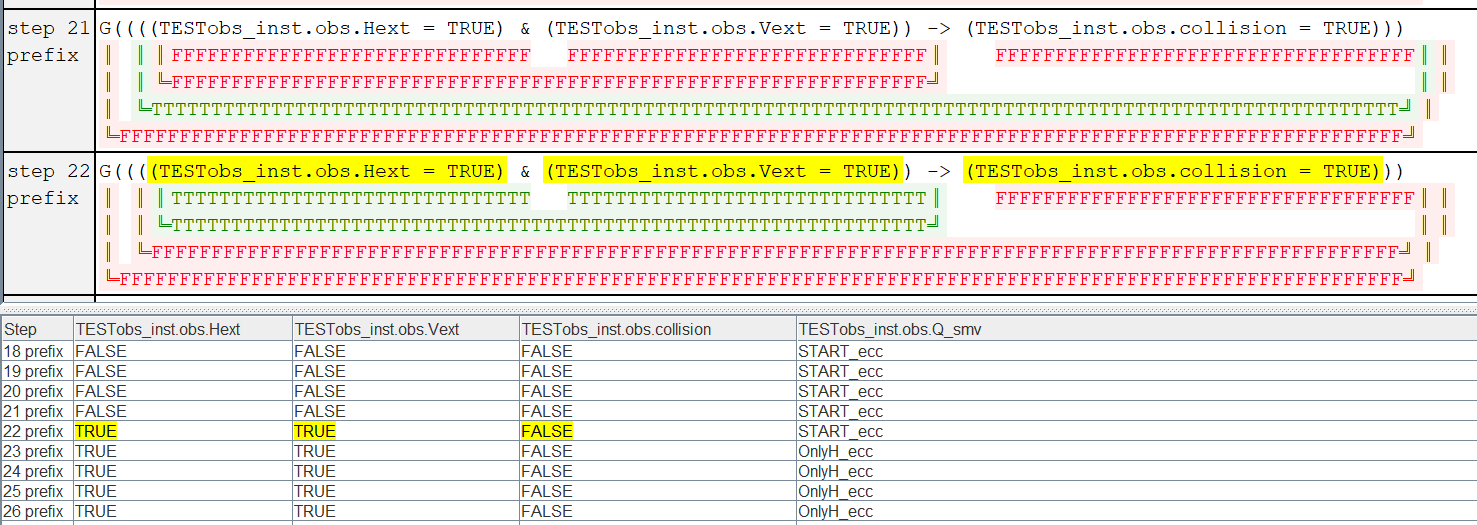
\includegraphics[width=0.9\textwidth]{MX_Papers/Paper3/pic/vizu_jumeauV1.png}
\caption{Analysis of the NuSMV counterexample trace in the FBME environment. The tool visualizes the system state at each step, highlights changes in the graphical FB network, and allows for causal analysis to trace the error back to its source.}
\label{fig:counterexample_analysis}
\end{figure}

The visual trace analysis in FBME made it possible to step through the failure scenario and clearly identify how the parallel execution, under a specific timing sequence explored by NuSMV due to the NDTs, led to the collision. This case study demonstrates the scalability and practical value of the integrated toolchain in ensuring the safety of complex, real-world industrial systems.

\section{Conclusion and Future Outlook}\label{sec:conclusion}

This chapter presented an integrated framework for the model-based design and formal verification of iCPS developed with the IEC 61499 standard. By combining a seamless toolchain with advanced modeling methodologies, the framework makes the power of formal verification more accessible to automation engineers, enabling the early detection of subtle and critical design flaws that traditional testing methods may miss.

The main contributions are threefold. First, the integrated toolchain provides a practical workflow from design and simulation in standard IDEs to automated formal model generation (fb2smv), verification (NuSMV), and intuitive counterexample analysis (FBME). Second, the proposed notation for Non-Deterministic Transitions (NDT) within IEC 61499 plant models allows for the creation of more realistic verification models that can uncover timing-dependent bugs. Third, the methodology for verifying runtime monitors using a non-deterministic twin of the controller ensures that online safety mechanisms are themselves reliable.

The application of this framework to multiple case studies, including a safety-critical nuclear handling system, has validated its effectiveness in improving the dependability of complex distributed automation systems. By lowering the barrier to entry for formal methods, this work contributes to building more robust, reliable, and safer industrial systems.

Future work will focus on extending the framework's capabilities. This includes automating the generation of ND twins for monitor verification and further exploring the scalability of the approach for even larger systems. Another promising direction is the extension of the modeling notation and toolchain to support timed automata, which would allow for the verification of quantitative real-time properties, moving beyond the current focus on logical correctness and untimed non-determinism. Finally, automatically generating specifications from informal requirements and generating plant models from system data logs are active research areas that could further enhance the automation and power of the verification process.


\makechapter{Nonsense chapter}{Nonsense chapter}{Nonsense chapter, here only to verify that some issues in previous versions are really resolved!}
\section{Process Mining Applications in Industrial Control Systems}

The integration of process mining techniques into industrial control systems represents a significant advancement in the field of cyber-physical systems, offering novel approaches to system modeling, verification, and control generation. Process mining, traditionally applied in business process management, has evolved to address the unique challenges of industrial automation, providing data-driven methods for understanding complex system behaviors and generating formal models from recorded event traces.

This chapter presents three complementary approaches that demonstrate the versatility and effectiveness of process mining in industrial control systems. The first approach focuses on process model extraction and conformance checking for anomaly detection and system monitoring. The second approach introduces an interactive learning methodology for automatic controller generation through simulation-based event recording. The third approach extends these capabilities to automatic plant model generation and real-time monitoring for formal verification.

These methodologies collectively address critical challenges in modern industrial automation: the need for automated system understanding, the complexity of controller development, and the requirement for formal verification in safety-critical applications. By leveraging process mining algorithms and the IEC 61499 standard, these approaches provide systematic methods for transforming recorded behavioral traces into formal models that can be used for system analysis, control generation, and verification.

\section{Process Model Extraction and Conformance Analysis}

The application of process mining techniques in industrial control systems begins with the fundamental challenge of understanding system behavior through recorded event logs. This approach leverages the inherent data-rich nature of modern automation systems to extract meaningful process models that can be used for system analysis, anomaly detection, and performance optimization.

\subsection{Process Mining Fundamentals in Industrial Contexts}

Process mining in industrial control systems differs fundamentally from its business process applications by focusing on the temporal and causal relationships between sensor and actuator signals rather than human activities. The core principle involves analyzing event logs that capture the sequence of control and sensor events occurring during system operation, then applying discovery algorithms to extract formal process models that represent the system's behavioral patterns.

The process mining workflow in industrial contexts typically involves three main phases: process discovery, conformance checking, and process enhancement. Process discovery algorithms analyze event logs to generate process models in various formalisms, most commonly Petri nets, which provide a mathematical foundation for representing concurrent and sequential behaviors. Conformance checking compares observed behavior against expected models to identify deviations, while process enhancement focuses on improving existing models based on new observations.

\begin{figure}[h]
    \centering
    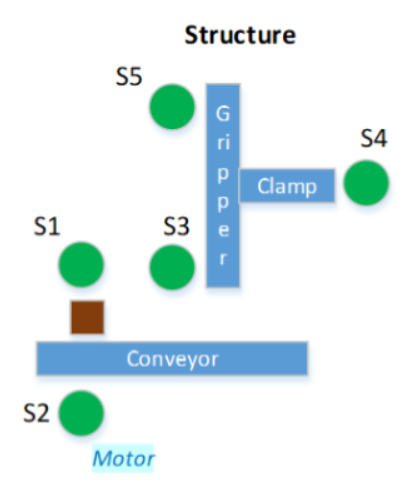
\includegraphics[width=0.8\textwidth]{MX_Papers/Paper5/images/structure.PNG}
    \caption{Gripper and conveyor system structure showing the integration of sensors and actuators in a typical industrial automation setup}
    \label{fig:gripper_conveyor_structure}
\end{figure}

The selection of appropriate process discovery algorithms is crucial for effective model extraction. Alpha algorithm, as a representative of abstraction-based methods, generates models by analyzing ordering relations between events in the log. This algorithm creates dependency graphs based on the sequence of events, making it suitable for systems with well-defined, deterministic behaviors. However, its sensitivity to noise in event logs can lead to overly complex models when dealing with systems that exhibit significant variability.

Heuristic-based algorithms, such as the fuzzy miner, offer an alternative approach that considers the frequency of event occurrences. These algorithms generate models based on the relative importance of activities and the strength of their relationships, making them more robust to noise and better suited for systems with complex, variable behaviors. The fuzzy miner, in particular, provides interactive representations that help understand system behavior in complex logs, though it may be more challenging to convert to other process modeling languages.

\subsection{Event Log Structure and Preprocessing}

The quality and structure of event logs significantly influence the effectiveness of process mining applications. Industrial control systems generate event logs that typically include case identifiers, timestamps, component information, signal names, and signal values. The case identifier represents unique process executions, often corresponding to complete operational cycles in cyclic manufacturing processes.

Event log preprocessing is essential for ensuring model quality and accuracy. This includes data cleaning to remove irrelevant events, format conversion to ensure compatibility with process mining tools, and attribute selection to focus on the most relevant information for the analysis. The conversion from CSV format to eXtensible Event Stream (XES) format is particularly important, as most process discovery algorithms require XES input.

\begin{figure}[h]
    \centering
    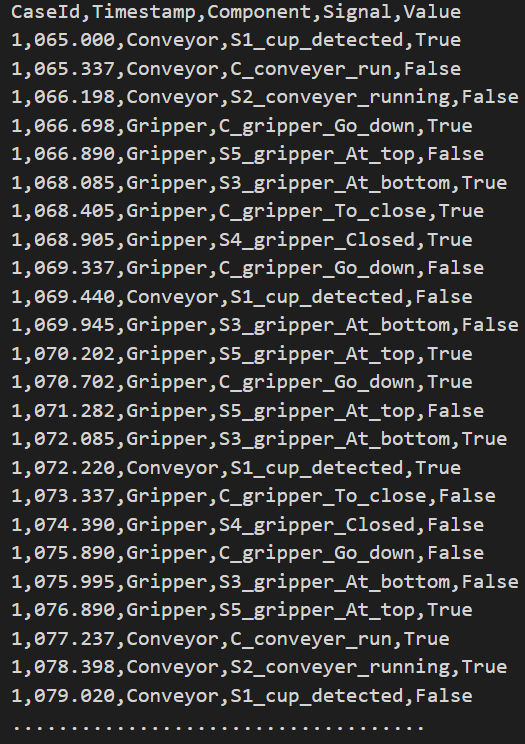
\includegraphics[width=0.7\textwidth]{MX_Papers/Paper5/images/EL.PNG}
    \caption{Event log structure showing the organization of case identifiers, timestamps, components, signals, and values in industrial control system data}
    \label{fig:event_log_structure}
\end{figure}

The preprocessing phase also involves mapping standard XES attributes to the industrial context. Case columns typically correspond to process execution identifiers, while event columns combine component, signal, and value information to create meaningful activity descriptions. This mapping ensures that the process mining algorithms can correctly interpret the industrial data and generate appropriate models.

\subsection{Conformance Checking and Anomaly Detection}

Conformance checking represents one of the most valuable applications of process mining in industrial control systems, providing systematic methods for detecting deviations from expected behavior. This capability is particularly important for anomaly detection, cyber-attack identification, and quality assurance in safety-critical applications.

The conformance checking process involves comparing observed event logs against reference process models to identify discrepancies. Several algorithms support this analysis, including causal footprint checking, token-based replay, and alignment-based methods. Causal footprint checking compares dependency matrices between the event log and reference model, providing a quick assessment of model fitness. However, this method does not consider event frequencies and may miss subtle deviations.

Token-based replay offers a more detailed analysis by simulating the execution of event traces on the reference model. This approach tracks missing and remaining tokens after each transition, providing quantitative measures of conformance. While effective, token replay has limitations when dealing with non-uniquely labeled transitions and can suffer from token flooding in complex models.

\begin{figure}[h]
    \centering
    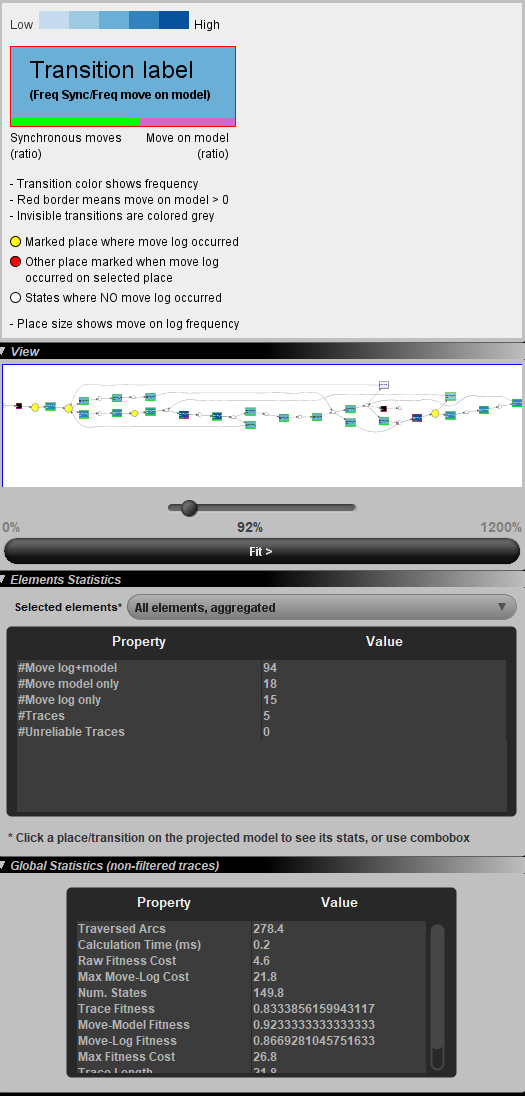
\includegraphics[width=0.6\textwidth]{MX_Papers/Paper5/images/stat1.PNG}
    \caption{Conformance checking results showing deviation analysis and fitness metrics for process model validation}
    \label{fig:conformance_checking_results}
\end{figure}

Alignment-based methods provide the most sophisticated approach to conformance checking, offering optimal alignment between observed and modeled behavior using user-defined cost functions. These methods are independent of process model notation and can handle complex scenarios that challenge other approaches. The alignment process identifies the optimal sequence of moves that transforms the observed trace into one that conforms to the model, providing detailed insights into the nature and location of deviations.

The application of conformance checking in industrial control systems extends beyond simple deviation detection to include performance analysis and system optimization. By analyzing conformance metrics over time, operators can identify trends in system behavior, detect gradual degradation, and optimize operational parameters. This capability is particularly valuable in predictive maintenance applications, where early detection of behavioral changes can prevent equipment failures and reduce downtime.

\section{Interactive Learning for Automatic Controller Generation}

The development of control logic for industrial automation systems traditionally requires significant domain expertise and manual programming effort. The interactive learning approach addresses this challenge by leveraging process mining techniques to automatically generate controllers from recorded behavioral traces, significantly reducing development time and improving system reliability.

\subsection{Simulation-Based Event Recording}

The foundation of interactive learning lies in the systematic recording of system behavior through simulation models. This approach uses 3D simulation environments, such as Visual Components, to create virtual representations of industrial systems that can be manipulated and observed without the risks and costs associated with physical experimentation.

The simulation environment provides a controlled setting where actuator signals can be manually triggered in appropriate sequences to generate desired process scenarios. Each interaction with the simulation model produces events that are recorded in chronological order, creating comprehensive behavioral traces that capture the complete system dynamics. This approach enables the generation of diverse process scenarios that might be difficult or dangerous to create in physical systems.

\begin{figure}[h]
    \centering
    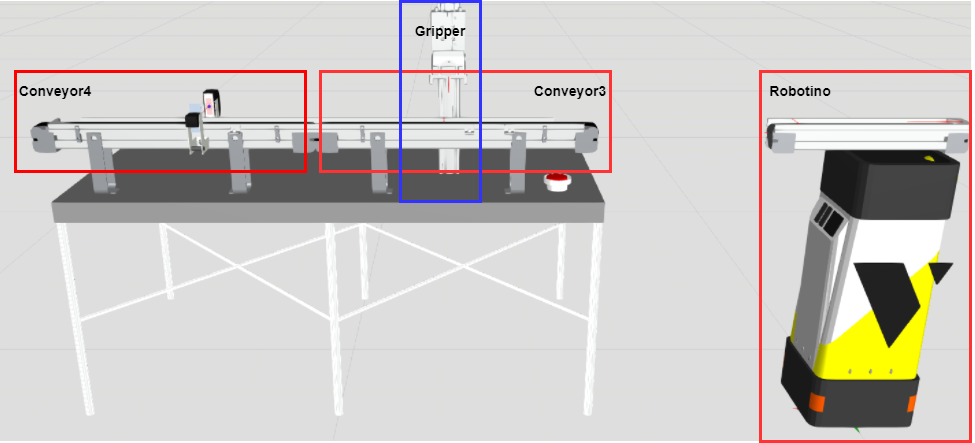
\includegraphics[width=0.7\textwidth]{MX_Papers/Paper6/images/simulation.png}
    \caption{3D simulation environment showing the production system with conveyor sections, gripper, and autonomous guided vehicle for interactive learning}
    \label{fig:simulation_environment}
\end{figure}

The recorded event logs capture the complete interaction between the simulation model and the operator, including sensor readings, actuator commands, and system state information. This comprehensive data collection ensures that the generated control logic accurately reflects the intended system behavior and can handle the full range of operational scenarios.

The simulation-based approach offers several advantages over traditional controller development methods. First, it eliminates the need for extensive domain knowledge in control system design, as the controller logic emerges directly from the recorded behavior. Second, it reduces development time by automating the transformation from behavioral requirements to executable control code. Third, it improves system reliability by ensuring that the controller logic is consistent with the observed system behavior.

\subsection{Process Discovery and Petri Net Generation}

The transformation from recorded event logs to executable control logic involves several systematic steps, beginning with process discovery to extract formal models from the behavioral traces. The alpha algorithm serves as the primary process discovery method, generating Petri nets that represent the system's behavioral patterns in a mathematically rigorous format.

The generated Petri nets capture the causal relationships between events, representing the system's state transitions and control flow. These models provide a formal foundation for understanding system behavior and serve as the basis for controller generation. The Petri net representation is particularly valuable because it can handle concurrent activities, sequential dependencies, and complex synchronization requirements that are common in industrial automation systems.

\begin{figure}[h]
    \centering
    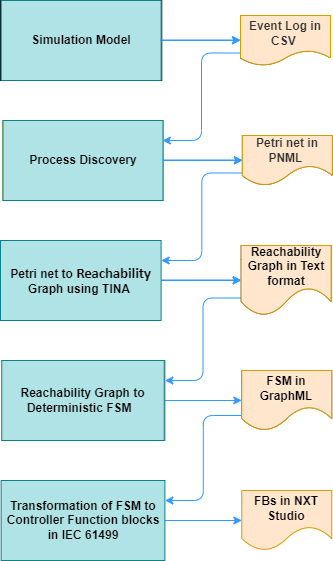
\includegraphics[width=0.8\textwidth]{MX_Papers/Paper6/images/PN2ControllerFlow.png}
    \caption{Methodology flow showing the transformation from event logs through Petri nets to IEC 61499 function blocks}
    \label{fig:methodology_flow}
\end{figure}

The Petri net generation process includes several important considerations. First, the addition of supplementary transitions, such as "Repeat" transitions, enables cyclic operation that is typical in manufacturing processes. Second, the stepwise simulation of the Petri net validates the model's correctness and ensures that it accurately represents the intended system behavior. Third, the conversion to reachability graphs provides a finite state machine representation that can be directly implemented in control systems.

The reachability graph represents all possible states and transitions of the system, providing a complete behavioral model that can be analyzed for properties such as deadlock freedom, liveness, and reachability. This analysis ensures that the generated controller will behave correctly under all operational conditions and can handle unexpected situations gracefully.

\subsection{Transformation to IEC 61499 Function Blocks}

The final step in the interactive learning process involves transforming the formal process models into executable IEC 61499 function blocks. This transformation requires careful mapping between the mathematical representation of the Petri net and the practical implementation requirements of industrial control systems.

The transformation process begins with the conversion of the reachability graph to a deterministic finite state machine (FSM). This conversion involves handling non-deterministic transitions, often represented as spontaneous or lambda transitions in the original Petri net. The determinization process ensures that the resulting FSM has unique transitions for each input combination, making it suitable for implementation in control systems.

\begin{figure}[h]
    \centering
    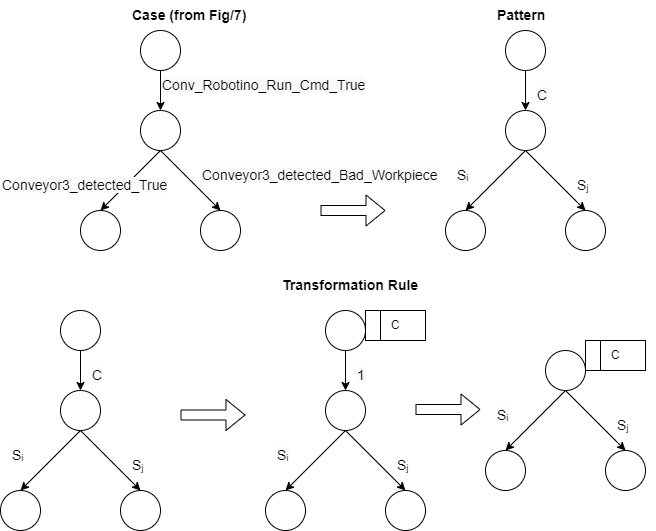
\includegraphics[width=0.7\textwidth]{MX_Papers/Paper6/images/UpdatedControllerConversionrules.png}
    \caption{FSM to ECC transformation rules showing the conversion from finite state machine to execution control chart}
    \label{fig:fsm_to_ecc_transformation}
\end{figure}

The transformation from FSM to IEC 61499 function blocks involves several key steps. First, the FSM states are mapped to ECC states in the function block. Second, the FSM transitions are converted to ECC transitions with appropriate conditions and actions. Third, the input and output events are defined based on the sensor and actuator signals identified in the original event log.

The resulting function block interface includes input events for all sensor signals and output events for all actuator signals. The ECC implements the control logic by defining state transitions that respond to sensor inputs and generate appropriate actuator outputs. This implementation ensures that the generated controller behaves exactly as recorded during the interactive learning process.

\begin{figure}[h]
    \centering
    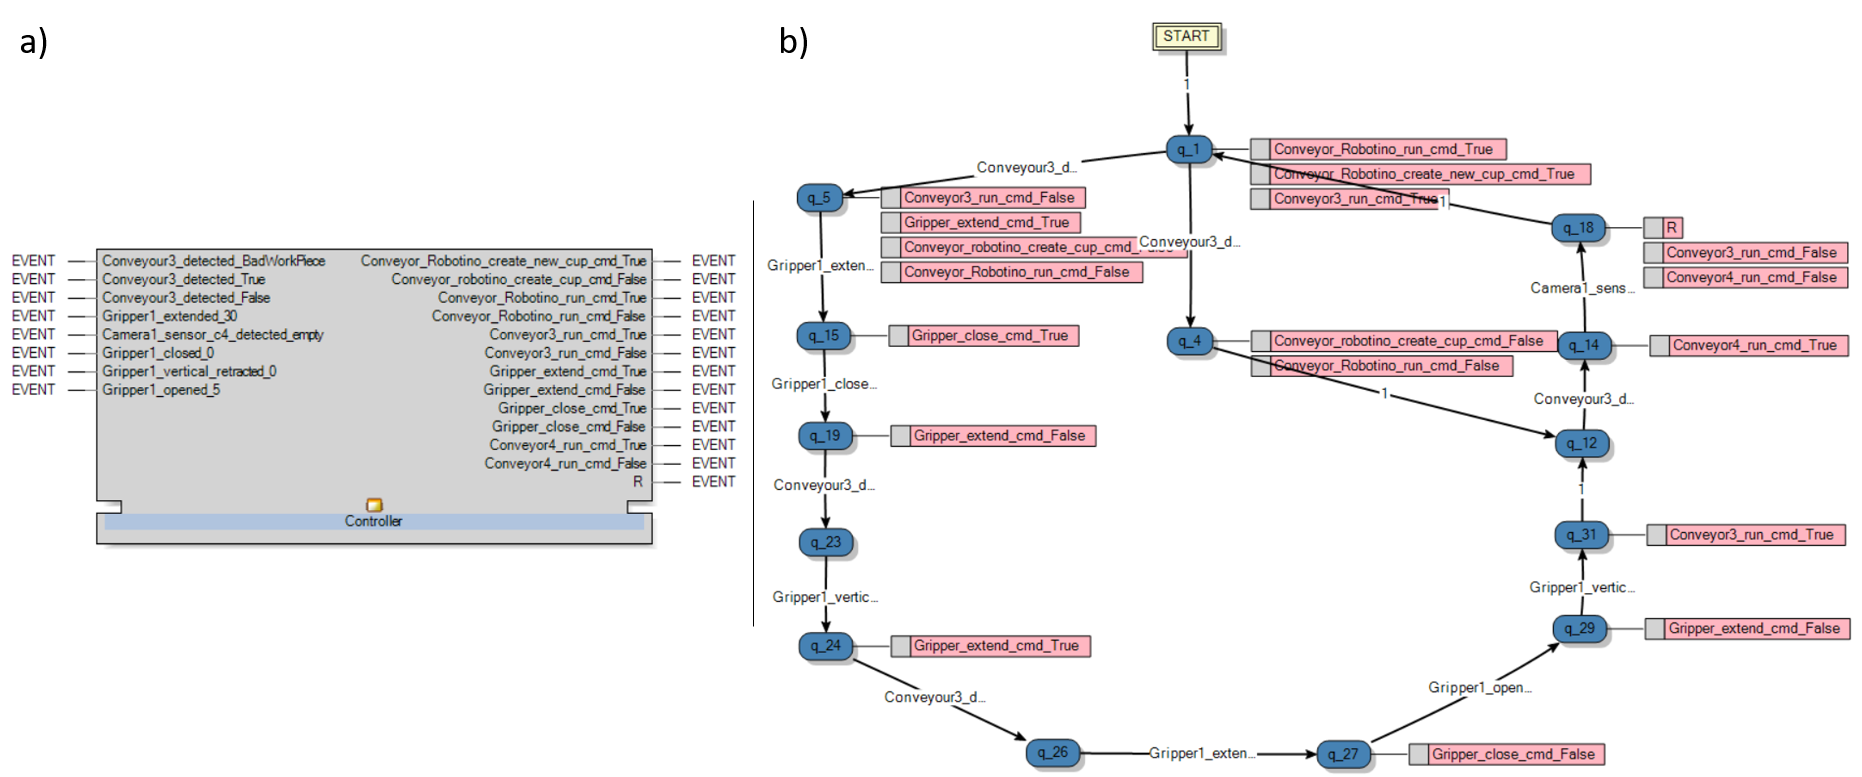
\includegraphics[width=0.9\textwidth]{MX_Papers/Paper6/images/FB.PNG}
    \caption{Generated IEC 61499 function block showing interface and ECC representation of the controller}
    \label{fig:generated_function_block}
\end{figure}

The interactive learning approach provides several significant advantages for controller development. First, it reduces development time by automating the transformation from behavioral requirements to executable code. Second, it improves system reliability by ensuring that the controller logic is consistent with observed system behavior. Third, it enables rapid prototyping and testing of different control strategies without extensive programming effort.

\section{Automatic Plant Model Generation and Real-Time Monitoring}

The extension of process mining techniques to automatic plant model generation represents a significant advancement in formal verification capabilities for industrial control systems. This approach addresses the critical challenge of creating accurate plant models for closed-loop system verification, enabling comprehensive analysis of system behavior and real-time monitoring of operational compliance.

\subsection{Reference Model of Control/Sensor Events Sequencing}

The foundation of automatic plant model generation lies in the Reference Model of Control/Sensor Events Sequencing (RMCSES), a formal model that represents the complete behavior of a closed-loop industrial automation system. This model is derived from process mining of event logs recorded during error-free system operation over extended periods.

The RMCSES provides a condensed representation of vast event logs, encompassing all possible signals from all system components. Conceptually, if the event log represents a collection of sentences describing system behavior, then RMCSES functions as a sentence generator for this formal language. This representation enables the model to be readily implemented in software or hardware, making it suitable for real-time applications.

\begin{figure}[h]
    \centering
    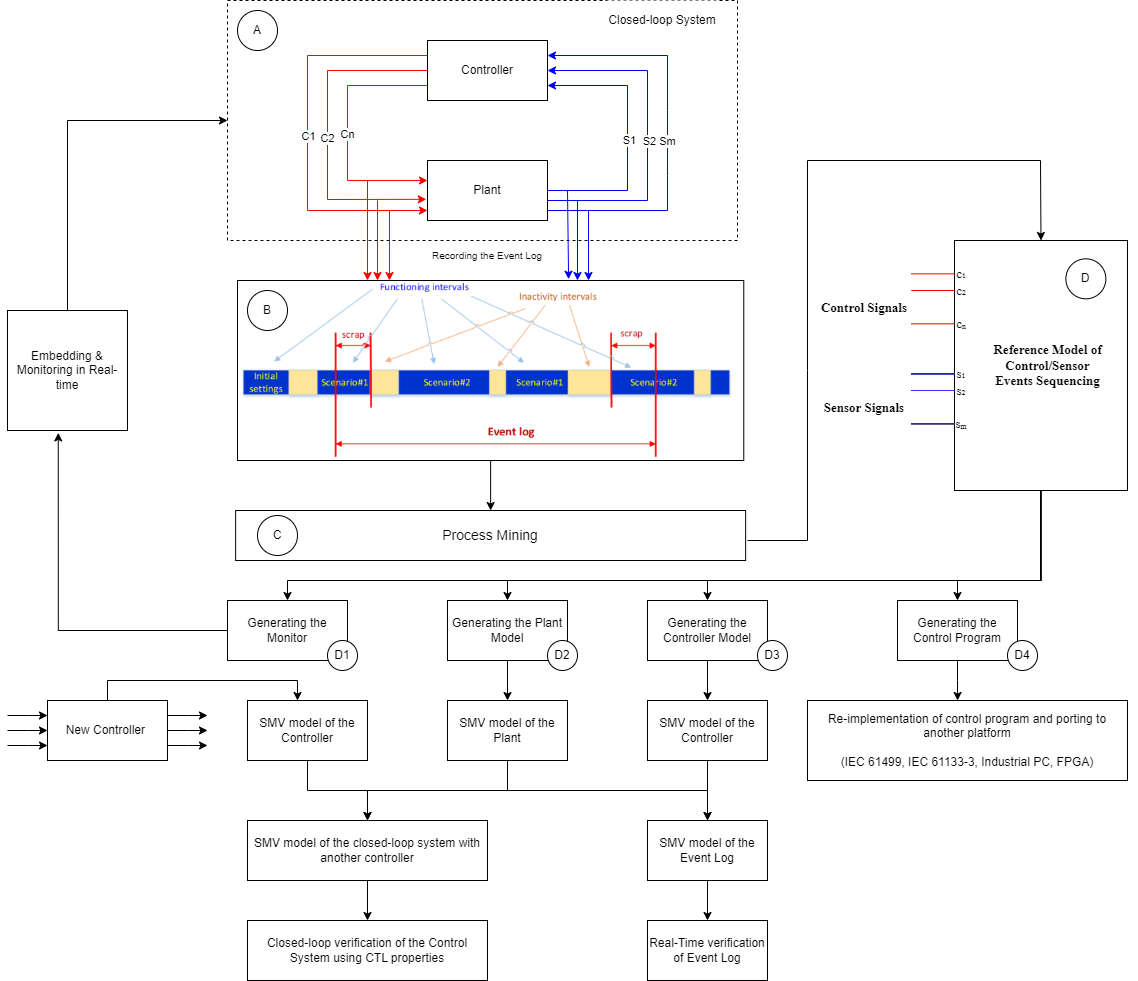
\includegraphics[width=0.9\textwidth]{MX_Papers/Paper7/images/workflow1.png}
    \caption{Workflow and use cases showing the transformation from event logs to monitor, plant model, control model, and control program}
    \label{fig:workflow_use_cases}
\end{figure}

The RMCSES interface focuses exclusively on control signals originating from the controller and informative signals originating from sensors, representing the interface between the controller and the plant. Internal signals circulating within the control system and plant are not considered, though control signals from external sources such as operators can be included. This focus on the controller-plant interface makes the model particularly suitable for closed-loop system analysis and verification.

The model assumes that each component in the system operates in a cyclical, meaningful, and locally complete manner. Components are considered to have meaningful behavior when they have specific goals and actively work toward achieving them. Each component follows specific scenarios that begin with initialization and end with termination, with multi-functional devices potentially executing different scenarios depending on their current task or operation.

\subsection{Petri Net Decomposition and State Machine Generation}

The transformation from event logs to plant models involves several sophisticated steps, beginning with Petri net construction and proceeding through decomposition and state machine generation. This process addresses the complexity of industrial systems by breaking down complex behaviors into manageable components while preserving essential behavioral characteristics.

The Petri net decomposition process utilizes reachability graph methods to identify subsets of states and transitions, facilitating the partitioning of complex Petri nets into manageable modules. This approach provides a structured and systematic method for exploring all reachable states and transitions within the system, ensuring completeness in capturing all potential behaviors.

\begin{figure}[h]
    \centering
    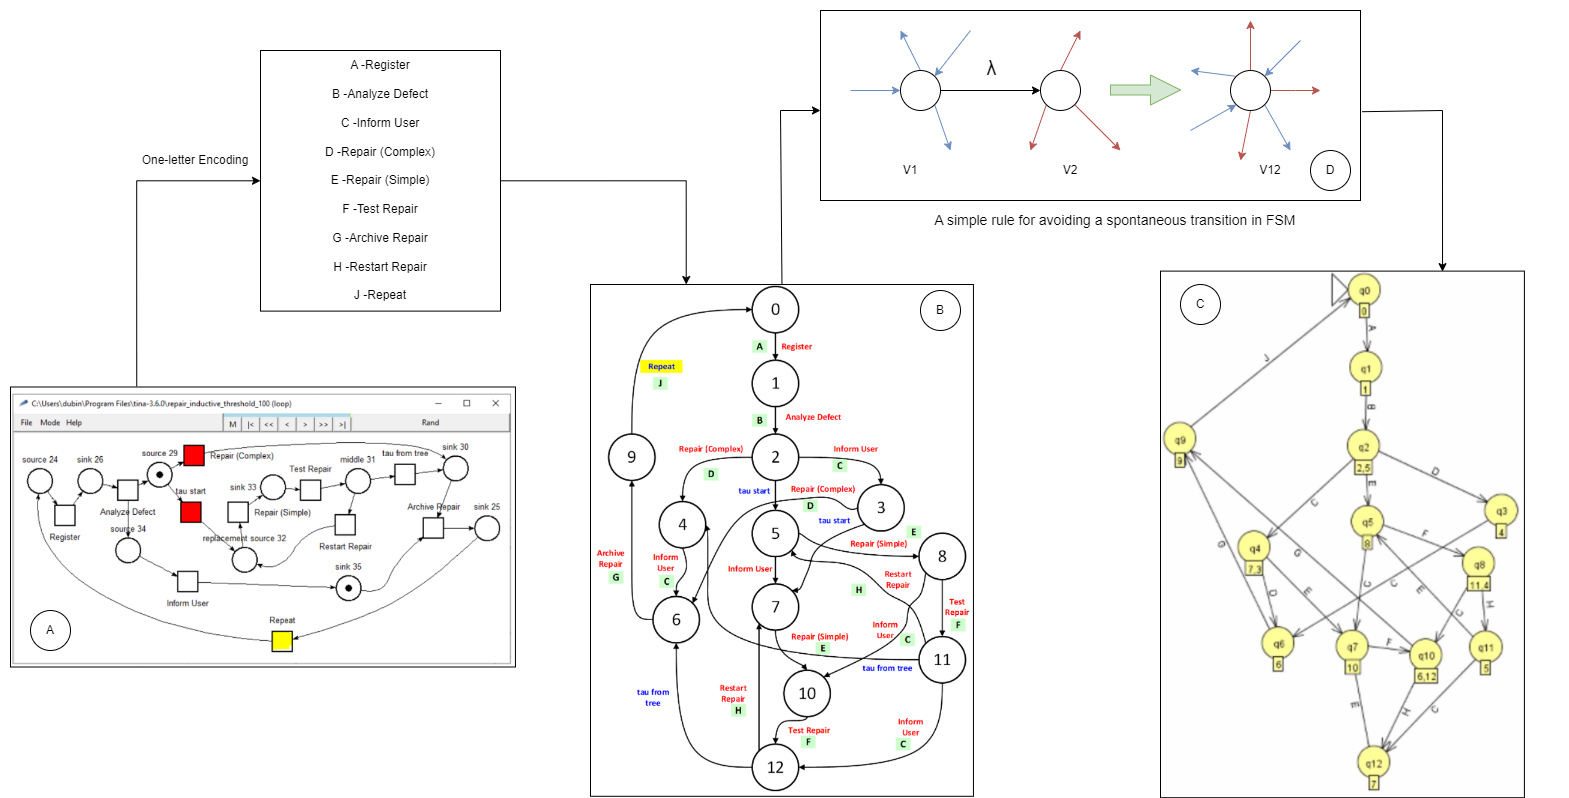
\includegraphics[width=0.8\textwidth]{MX_Papers/Paper7/images/PN2FSM.png}
    \caption{Transformation of Petri net to FSM showing the decomposition process and state machine generation}
    \label{fig:petri_net_to_fsm}
\end{figure}

The reachability graph method, while comprehensive, can suffer from state space explosion in complex systems. To address this challenge, several strategies are employed: state space reduction using symbolic representations such as Binary Decision Diagrams (BDDs), abstraction and aggregation methods that focus on essential behavioral properties, partial order reduction techniques that avoid redundant interleavings, and on-the-fly exploration that generates states as needed.

The composition of State Machine Components (SMCs) into a cohesive FSM requires careful integration to ensure synchronization and coordination. Parallel composition and synchronization techniques are preferred for IEC 61499 systems, as they align with the distributed and modular architecture of these systems. This approach enables concurrent execution of SMCs while maintaining proper coordination and communication between distributed components.

\subsection{Monitor Implementation for Real-Time Conformance Checking}

The automatic generation of monitors represents a critical application of the RMCSES, enabling real-time detection of deviations from expected system behavior. These monitors are implemented as IEC 61499 function blocks that can be deployed in operational systems to provide continuous monitoring and early warning of potential issues.

The monitor implementation involves transforming the RMCSES into a function block that receives input signals from both controller and sensor components. The monitor's ECC is generated using transformation rules that map FSM states and transitions to appropriate ECC states and transitions. When the monitor detects a valid transition, it generates an "OK" output indicating successful operation. If an unexpected event occurs, the monitor transitions to an error state and produces an "ERROR" event with details about the event that caused the error.

\begin{figure}[h]
    \centering
    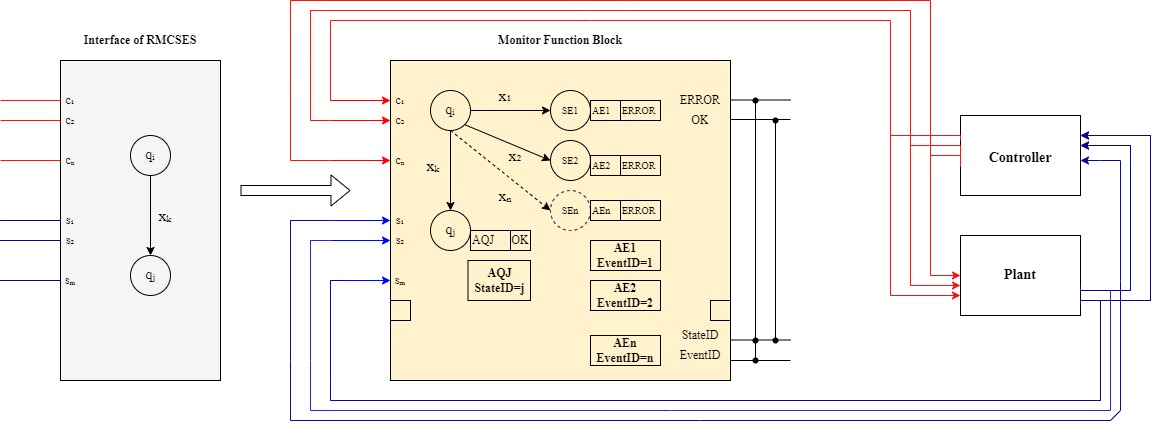
\includegraphics[width=0.9\textwidth]{MX_Papers/Paper7/images/ConformaceCheckingApp.jpg}
    \caption{Application for conformance checking showing the integration of monitor with closed-loop system}
    \label{fig:conformance_checking_app}
\end{figure}

The monitor's error detection capabilities are comprehensive, covering all possible input events from each state. For each state in the FSM, the monitor defines transitions to error states for all input events that are not specified in the reference model. This complete coverage ensures that any deviation from expected behavior is detected immediately, providing robust protection against system malfunctions and unauthorized operations.

The monitor implementation includes several important features. First, it provides detailed error information including the state where the error occurred and the specific event that caused the error. Second, it continues operation until the first error is detected, after which it becomes non-responsive to prevent further processing. Third, it can be easily integrated with existing control systems without requiring significant modifications to the operational infrastructure.

\subsection{Plant Model Generation for Formal Verification}

The automatic generation of plant models extends the capabilities of process mining to formal verification applications. These plant models represent the uncontrolled behavior of the physical system and can be integrated with control models to create complete closed-loop system representations suitable for formal analysis.

The plant model generation process involves extracting the uncontrolled plant behavior from the overall system model represented by the RMCSES. This extraction requires careful analysis to distinguish between control-driven and sensor-driven transitions, as the plant model should only respond to control signals and generate sensor signals based on its internal state.

\begin{figure}[h]
    \centering
    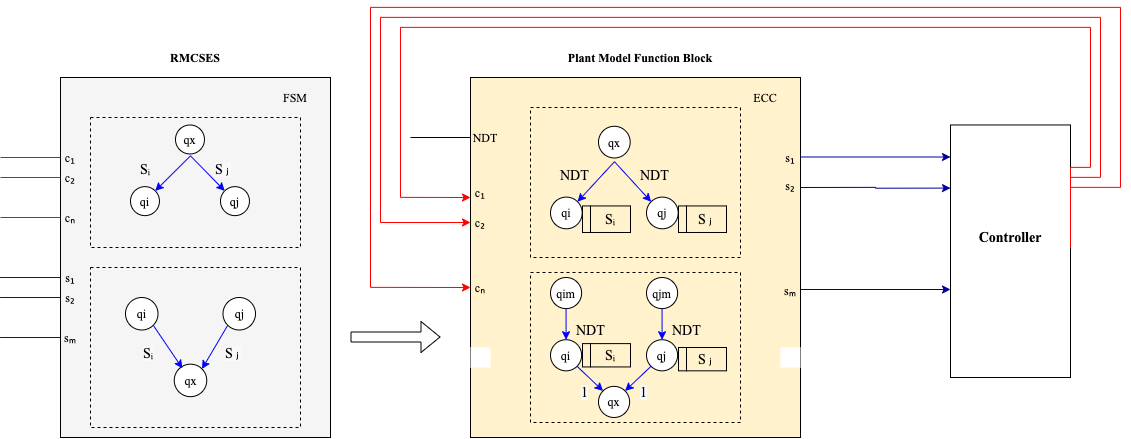
\includegraphics[width=0.9\textwidth]{MX_Papers/Paper7/images/VerificationApp1.png}
    \caption{Application for verification showing the integration of plant model with controller for formal analysis}
    \label{fig:verification_app}
\end{figure}

The transformation from FSM to plant model involves specific rules for handling sensor and control signals. Transitions triggered by sensor signals are replaced with non-deterministic transitions (NDT) that can fire at arbitrary time intervals, with the output of the next state serving as a sensor event signal. Control signal transitions remain unchanged, as the plant should respond directly to control inputs.

The plant model implementation addresses several important challenges. First, it handles diverging sensor signals by creating separate NDT transitions for each possible sensor output. Second, it manages converging sensor signals by introducing intermediate states that produce appropriate sensor signals before converging to the target state. Third, it maintains the non-deterministic nature of plant behavior while providing a deterministic interface for integration with control systems.

The generated plant model can be used for formal verification using tools such as NuSMV and CTL/LTL specifications. The model can be converted to SMV format using the fb2smv tool, enabling comprehensive analysis of system properties including safety, liveness, and reachability. This verification capability is particularly valuable for safety-critical applications where formal guarantees of system behavior are required.

\section{Integration and Applications}

The three approaches presented in this chapter represent complementary aspects of process mining applications in industrial control systems, each addressing different challenges in system understanding, control generation, and verification. Their integration provides a comprehensive framework for addressing the complex requirements of modern industrial automation.

\subsection{Comprehensive System Analysis Framework}

The integration of process model extraction, interactive learning, and automatic plant model generation creates a comprehensive framework for industrial control system analysis and development. This framework enables end-to-end system understanding, from initial behavior recording through formal verification and operational monitoring.

The framework begins with process model extraction, which provides fundamental understanding of system behavior through analysis of recorded event logs. This understanding serves as the foundation for both controller generation and plant model development, ensuring consistency across all system representations.

Interactive learning builds upon this foundation by enabling automatic controller generation from recorded behavioral traces. This approach reduces development time and improves system reliability by ensuring that control logic is consistent with observed system behavior. The generated controllers can be immediately deployed or used as starting points for further refinement.

Automatic plant model generation extends the framework to formal verification applications, enabling comprehensive analysis of closed-loop system behavior. The generated plant models can be used with existing or newly developed controllers to verify system properties and ensure compliance with safety and performance requirements.

\subsection{Industrial Applications and Case Studies}

The presented approaches have been validated through several industrial case studies, demonstrating their effectiveness in real-world applications. The gripper and conveyor system case study illustrates the application of process model extraction for system understanding and anomaly detection. This case study shows how process mining can be used to analyze complex manufacturing processes and identify potential improvements in system operation.

The interactive learning case study demonstrates the application of simulation-based controller generation for a production system with multiple components including conveyors, grippers, and autonomous guided vehicles. This case study shows how the approach can handle complex, multi-component systems and generate controllers that accurately reflect desired system behavior.

The pneumatic cylinder case study illustrates the application of automatic plant model generation and real-time monitoring. This case study shows how the approach can be used for formal verification of safety-critical systems and real-time monitoring of operational compliance.

\begin{figure}[h]
    \centering
    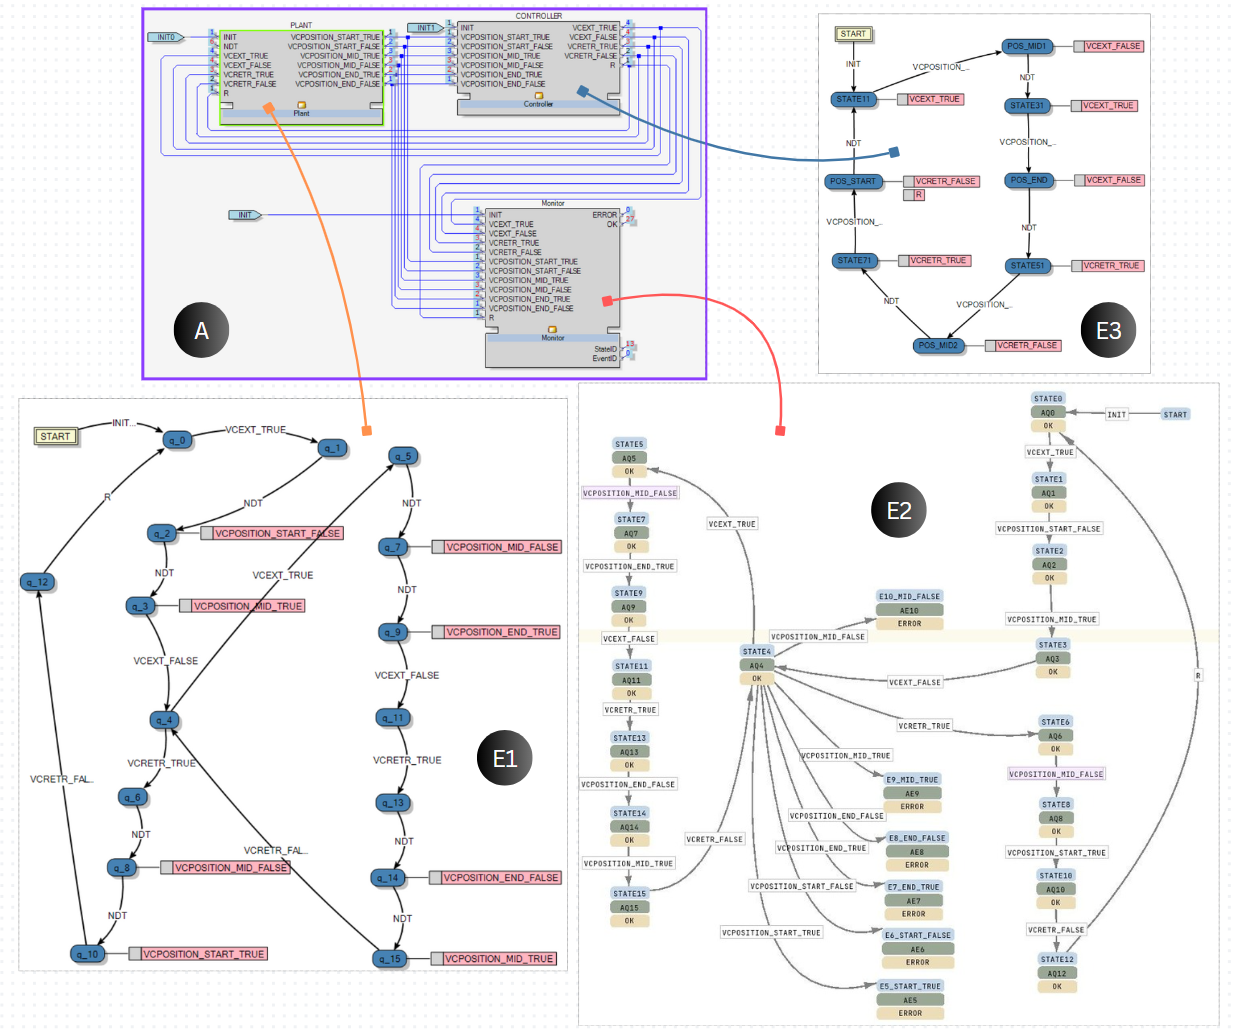
\includegraphics[width=0.8\textwidth]{MX_Papers/Paper7/images/CLMC.PNG}
    \caption{Closed-loop system integration showing plant model, controller, and monitor working together for comprehensive system analysis}
    \label{fig:closed_loop_integration}
\end{figure}

These case studies demonstrate the versatility of the presented approaches and their applicability to a wide range of industrial applications. The approaches can be adapted to different system types, from simple single-component systems to complex multi-component manufacturing lines, providing flexible solutions for various industrial automation challenges.

\subsection{Future Research Directions}

The integration of process mining with industrial control systems opens several promising research directions that could further enhance the capabilities and applicability of these approaches.

First, the development of more sophisticated process discovery algorithms could improve the quality and accuracy of generated models. Current algorithms may struggle with complex, highly concurrent systems or systems with significant noise in their event logs. Advanced algorithms that can handle these challenges would expand the applicability of the approaches to a broader range of industrial systems.

Second, the integration of machine learning techniques with process mining could enable adaptive models that improve over time based on new observations. This capability would be particularly valuable for systems that evolve or change their behavior over time, enabling continuous improvement of system understanding and control.

Third, the development of more efficient algorithms for handling large-scale event logs could enable the application of these approaches to complex, multi-facility manufacturing systems. Current approaches may face computational challenges when dealing with very large event logs or complex system architectures.

Fourth, the integration of these approaches with emerging technologies such as digital twins and edge computing could enable real-time process mining and control generation. This integration would enable dynamic adaptation of control systems based on real-time analysis of system behavior, providing more responsive and adaptive automation solutions.

The research presented in this chapter demonstrates the significant potential of process mining techniques for addressing critical challenges in industrial control systems. The three complementary approaches provide comprehensive solutions for system understanding, control generation, and verification, while the integration of these approaches creates a powerful framework for industrial automation development and analysis.

As industrial systems become increasingly complex and interconnected, the need for automated methods for system understanding and control generation will continue to grow. The approaches presented in this chapter provide a solid foundation for addressing these challenges and enable the development of more intelligent, adaptive, and reliable industrial automation systems.

The future of industrial automation lies in the integration of data-driven approaches with formal methods, creating systems that can learn from their environment, adapt to changing requirements, and provide formal guarantees of their behavior. The process mining approaches presented in this chapter represent important steps toward this vision, providing practical methods for realizing intelligent industrial automation systems that can meet the demands of modern manufacturing.


\makechapter{Nonsense chapter}{Nonsense chapter}{Nonsense chapter, here only to verify that some issues in previous versions are really resolved!}
%\section{Process Mining Applications in Industrial Control Systems}

The integration of process mining techniques into industrial control systems represents a significant advancement in the field of cyber-physical systems, offering novel approaches to system modeling, verification, and control generation. Process mining, traditionally applied in business process management, has evolved to address the unique challenges of industrial automation, providing data-driven methods for understanding complex system behaviors and generating formal models from recorded event traces.

This chapter presents three complementary approaches that demonstrate the versatility and effectiveness of process mining in industrial control systems. The first approach focuses on process model extraction and conformance checking for anomaly detection and system monitoring. The second approach introduces an interactive learning methodology for automatic controller generation through simulation-based event recording. The third approach extends these capabilities to automatic plant model generation and real-time monitoring for formal verification.

These methodologies collectively address critical challenges in modern industrial automation: the need for automated system understanding, the complexity of controller development, and the requirement for formal verification in safety-critical applications. By leveraging process mining algorithms and the IEC 61499 standard, these approaches provide systematic methods for transforming recorded behavioral traces into formal models that can be used for system analysis, control generation, and verification.

\section{Process Model Extraction and Conformance Analysis}

The application of process mining techniques in industrial control systems begins with the fundamental challenge of understanding system behavior through recorded event logs. This approach leverages the inherent data-rich nature of modern automation systems to extract meaningful process models that can be used for system analysis, anomaly detection, and performance optimization.

\subsection{Process Mining Fundamentals in Industrial Contexts}

Process mining in industrial control systems differs fundamentally from its business process applications by focusing on the temporal and causal relationships between sensor and actuator signals rather than human activities. The core principle involves analyzing event logs that capture the sequence of control and sensor events occurring during system operation, then applying discovery algorithms to extract formal process models that represent the system's behavioral patterns.

The process mining workflow in industrial contexts typically involves three main phases: process discovery, conformance checking, and process enhancement. Process discovery algorithms analyze event logs to generate process models in various formalisms, most commonly Petri nets, which provide a mathematical foundation for representing concurrent and sequential behaviors. Conformance checking compares observed behavior against expected models to identify deviations, while process enhancement focuses on improving existing models based on new observations.

\begin{figure}[h]
    \centering
    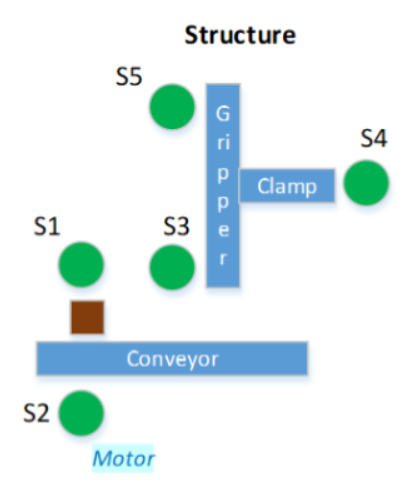
\includegraphics[width=0.8\textwidth]{MX_Papers/Paper5/images/structure.PNG}
    \caption{Gripper and conveyor system structure showing the integration of sensors and actuators in a typical industrial automation setup}
    \label{fig:gripper_conveyor_structure}
\end{figure}

The selection of appropriate process discovery algorithms is crucial for effective model extraction. Alpha algorithm, as a representative of abstraction-based methods, generates models by analyzing ordering relations between events in the log. This algorithm creates dependency graphs based on the sequence of events, making it suitable for systems with well-defined, deterministic behaviors. However, its sensitivity to noise in event logs can lead to overly complex models when dealing with systems that exhibit significant variability.

Heuristic-based algorithms, such as the fuzzy miner, offer an alternative approach that considers the frequency of event occurrences. These algorithms generate models based on the relative importance of activities and the strength of their relationships, making them more robust to noise and better suited for systems with complex, variable behaviors. The fuzzy miner, in particular, provides interactive representations that help understand system behavior in complex logs, though it may be more challenging to convert to other process modeling languages.

\subsection{Event Log Structure and Preprocessing}

The quality and structure of event logs significantly influence the effectiveness of process mining applications. Industrial control systems generate event logs that typically include case identifiers, timestamps, component information, signal names, and signal values. The case identifier represents unique process executions, often corresponding to complete operational cycles in cyclic manufacturing processes.

Event log preprocessing is essential for ensuring model quality and accuracy. This includes data cleaning to remove irrelevant events, format conversion to ensure compatibility with process mining tools, and attribute selection to focus on the most relevant information for the analysis. The conversion from CSV format to eXtensible Event Stream (XES) format is particularly important, as most process discovery algorithms require XES input.

\begin{figure}[h]
    \centering
    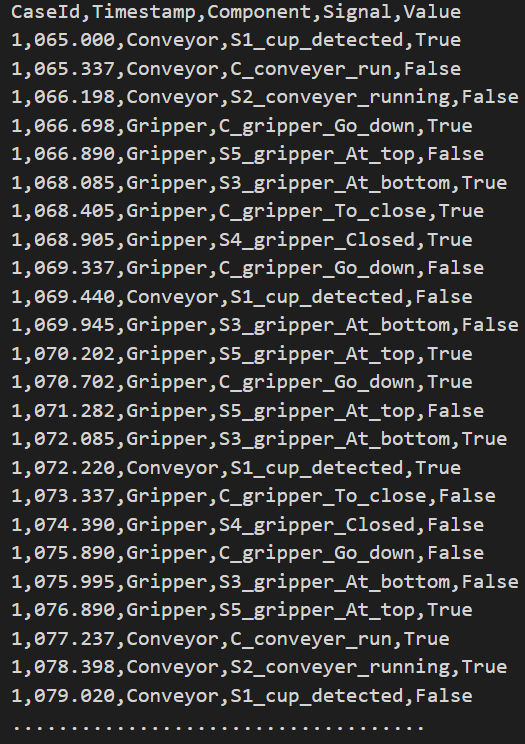
\includegraphics[width=0.7\textwidth]{MX_Papers/Paper5/images/EL.PNG}
    \caption{Event log structure showing the organization of case identifiers, timestamps, components, signals, and values in industrial control system data}
    \label{fig:event_log_structure}
\end{figure}

The preprocessing phase also involves mapping standard XES attributes to the industrial context. Case columns typically correspond to process execution identifiers, while event columns combine component, signal, and value information to create meaningful activity descriptions. This mapping ensures that the process mining algorithms can correctly interpret the industrial data and generate appropriate models.

\subsection{Conformance Checking and Anomaly Detection}

Conformance checking represents one of the most valuable applications of process mining in industrial control systems, providing systematic methods for detecting deviations from expected behavior. This capability is particularly important for anomaly detection, cyber-attack identification, and quality assurance in safety-critical applications.

The conformance checking process involves comparing observed event logs against reference process models to identify discrepancies. Several algorithms support this analysis, including causal footprint checking, token-based replay, and alignment-based methods. Causal footprint checking compares dependency matrices between the event log and reference model, providing a quick assessment of model fitness. However, this method does not consider event frequencies and may miss subtle deviations.

Token-based replay offers a more detailed analysis by simulating the execution of event traces on the reference model. This approach tracks missing and remaining tokens after each transition, providing quantitative measures of conformance. While effective, token replay has limitations when dealing with non-uniquely labeled transitions and can suffer from token flooding in complex models.

\begin{figure}[h]
    \centering
    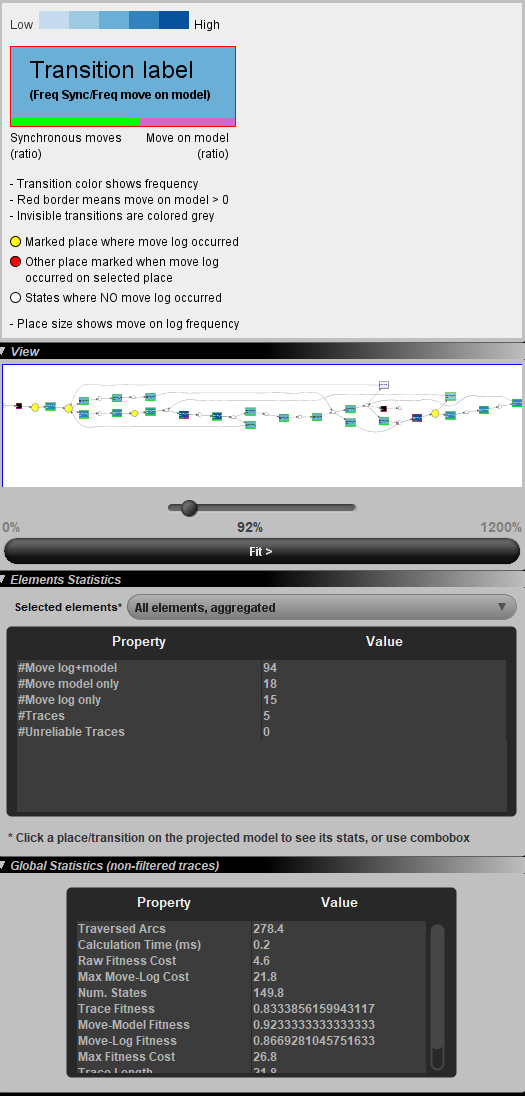
\includegraphics[width=0.6\textwidth]{MX_Papers/Paper5/images/stat1.PNG}
    \caption{Conformance checking results showing deviation analysis and fitness metrics for process model validation}
    \label{fig:conformance_checking_results}
\end{figure}

Alignment-based methods provide the most sophisticated approach to conformance checking, offering optimal alignment between observed and modeled behavior using user-defined cost functions. These methods are independent of process model notation and can handle complex scenarios that challenge other approaches. The alignment process identifies the optimal sequence of moves that transforms the observed trace into one that conforms to the model, providing detailed insights into the nature and location of deviations.

The application of conformance checking in industrial control systems extends beyond simple deviation detection to include performance analysis and system optimization. By analyzing conformance metrics over time, operators can identify trends in system behavior, detect gradual degradation, and optimize operational parameters. This capability is particularly valuable in predictive maintenance applications, where early detection of behavioral changes can prevent equipment failures and reduce downtime.

\section{Interactive Learning for Automatic Controller Generation}

The development of control logic for industrial automation systems traditionally requires significant domain expertise and manual programming effort. The interactive learning approach addresses this challenge by leveraging process mining techniques to automatically generate controllers from recorded behavioral traces, significantly reducing development time and improving system reliability.

\subsection{Simulation-Based Event Recording}

The foundation of interactive learning lies in the systematic recording of system behavior through simulation models. This approach uses 3D simulation environments, such as Visual Components, to create virtual representations of industrial systems that can be manipulated and observed without the risks and costs associated with physical experimentation.

The simulation environment provides a controlled setting where actuator signals can be manually triggered in appropriate sequences to generate desired process scenarios. Each interaction with the simulation model produces events that are recorded in chronological order, creating comprehensive behavioral traces that capture the complete system dynamics. This approach enables the generation of diverse process scenarios that might be difficult or dangerous to create in physical systems.

\begin{figure}[h]
    \centering
    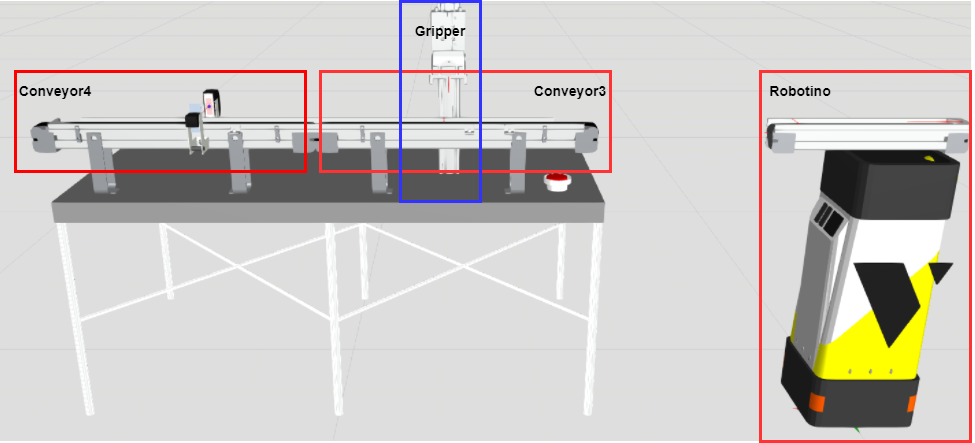
\includegraphics[width=0.7\textwidth]{MX_Papers/Paper6/images/simulation.png}
    \caption{3D simulation environment showing the production system with conveyor sections, gripper, and autonomous guided vehicle for interactive learning}
    \label{fig:simulation_environment}
\end{figure}

The recorded event logs capture the complete interaction between the simulation model and the operator, including sensor readings, actuator commands, and system state information. This comprehensive data collection ensures that the generated control logic accurately reflects the intended system behavior and can handle the full range of operational scenarios.

The simulation-based approach offers several advantages over traditional controller development methods. First, it eliminates the need for extensive domain knowledge in control system design, as the controller logic emerges directly from the recorded behavior. Second, it reduces development time by automating the transformation from behavioral requirements to executable control code. Third, it improves system reliability by ensuring that the controller logic is consistent with the observed system behavior.

\subsection{Process Discovery and Petri Net Generation}

The transformation from recorded event logs to executable control logic involves several systematic steps, beginning with process discovery to extract formal models from the behavioral traces. The alpha algorithm serves as the primary process discovery method, generating Petri nets that represent the system's behavioral patterns in a mathematically rigorous format.

The generated Petri nets capture the causal relationships between events, representing the system's state transitions and control flow. These models provide a formal foundation for understanding system behavior and serve as the basis for controller generation. The Petri net representation is particularly valuable because it can handle concurrent activities, sequential dependencies, and complex synchronization requirements that are common in industrial automation systems.

\begin{figure}[h]
    \centering
    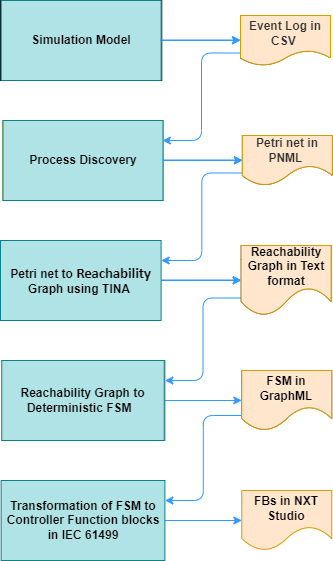
\includegraphics[width=0.8\textwidth]{MX_Papers/Paper6/images/PN2ControllerFlow.png}
    \caption{Methodology flow showing the transformation from event logs through Petri nets to IEC 61499 function blocks}
    \label{fig:methodology_flow}
\end{figure}

The Petri net generation process includes several important considerations. First, the addition of supplementary transitions, such as "Repeat" transitions, enables cyclic operation that is typical in manufacturing processes. Second, the stepwise simulation of the Petri net validates the model's correctness and ensures that it accurately represents the intended system behavior. Third, the conversion to reachability graphs provides a finite state machine representation that can be directly implemented in control systems.

The reachability graph represents all possible states and transitions of the system, providing a complete behavioral model that can be analyzed for properties such as deadlock freedom, liveness, and reachability. This analysis ensures that the generated controller will behave correctly under all operational conditions and can handle unexpected situations gracefully.

\subsection{Transformation to IEC 61499 Function Blocks}

The final step in the interactive learning process involves transforming the formal process models into executable IEC 61499 function blocks. This transformation requires careful mapping between the mathematical representation of the Petri net and the practical implementation requirements of industrial control systems.

The transformation process begins with the conversion of the reachability graph to a deterministic finite state machine (FSM). This conversion involves handling non-deterministic transitions, often represented as spontaneous or lambda transitions in the original Petri net. The determinization process ensures that the resulting FSM has unique transitions for each input combination, making it suitable for implementation in control systems.

\begin{figure}[h]
    \centering
    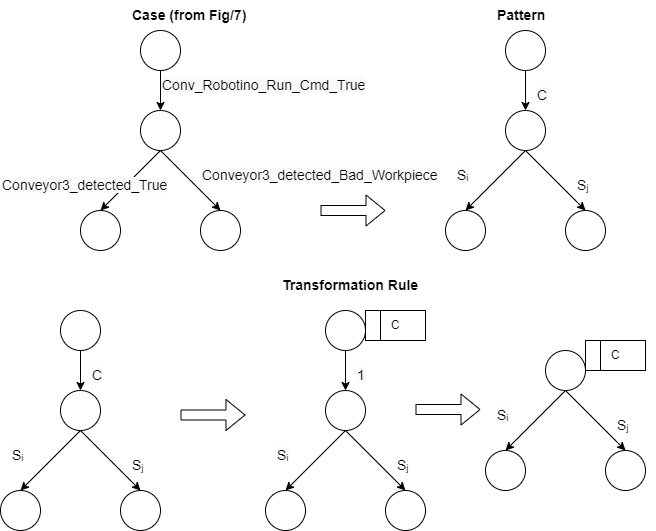
\includegraphics[width=0.7\textwidth]{MX_Papers/Paper6/images/UpdatedControllerConversionrules.png}
    \caption{FSM to ECC transformation rules showing the conversion from finite state machine to execution control chart}
    \label{fig:fsm_to_ecc_transformation}
\end{figure}

The transformation from FSM to IEC 61499 function blocks involves several key steps. First, the FSM states are mapped to ECC states in the function block. Second, the FSM transitions are converted to ECC transitions with appropriate conditions and actions. Third, the input and output events are defined based on the sensor and actuator signals identified in the original event log.

The resulting function block interface includes input events for all sensor signals and output events for all actuator signals. The ECC implements the control logic by defining state transitions that respond to sensor inputs and generate appropriate actuator outputs. This implementation ensures that the generated controller behaves exactly as recorded during the interactive learning process.

\begin{figure}[h]
    \centering
    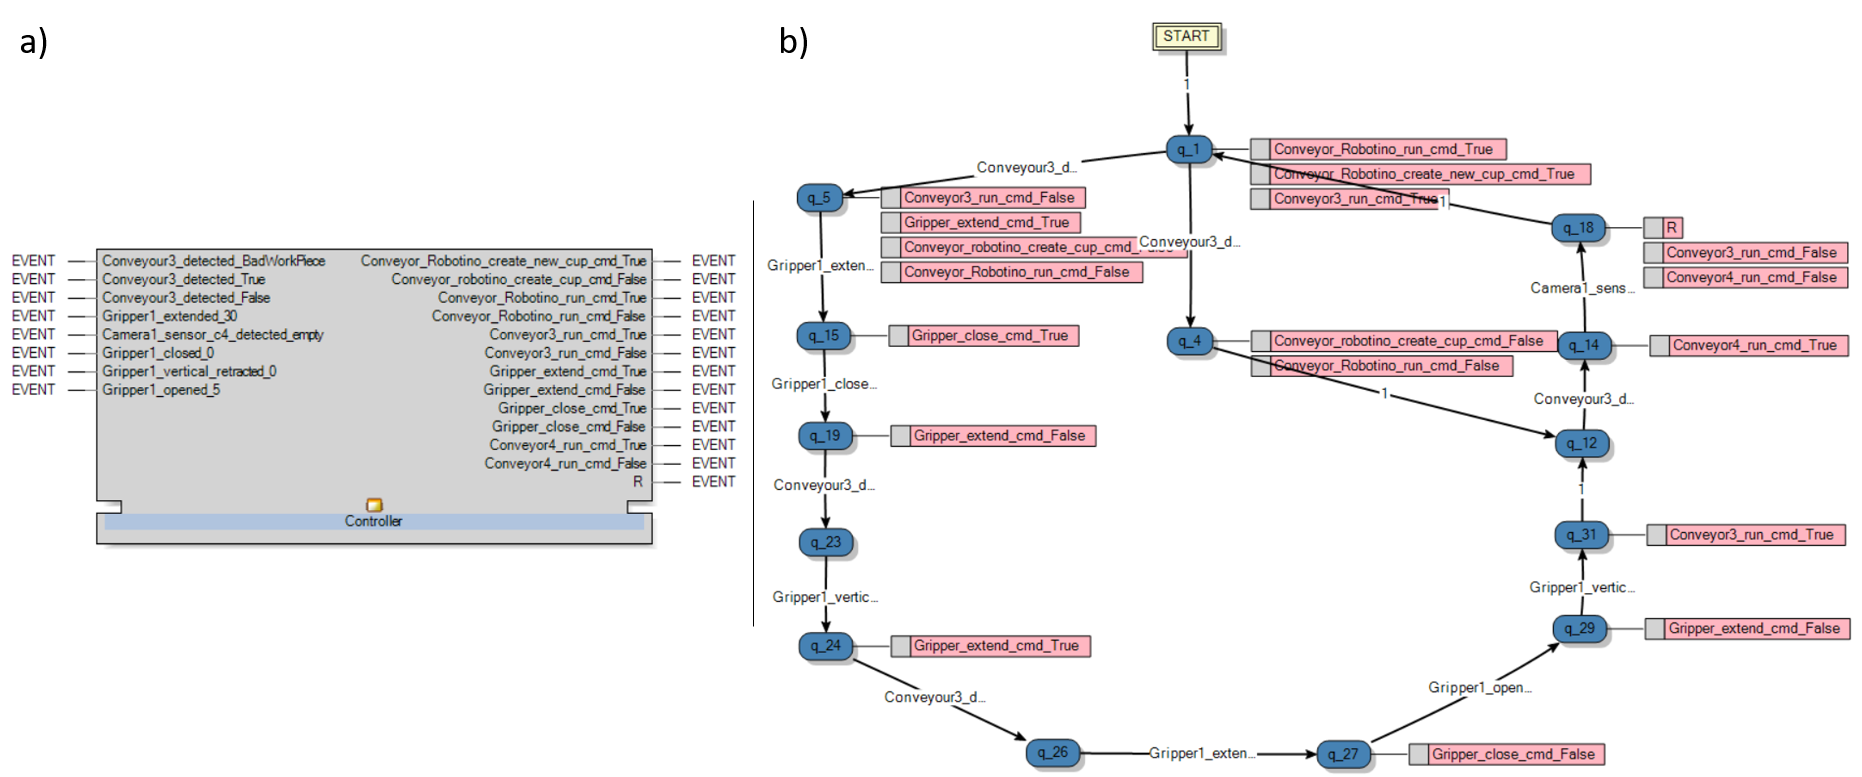
\includegraphics[width=0.9\textwidth]{MX_Papers/Paper6/images/FB.PNG}
    \caption{Generated IEC 61499 function block showing interface and ECC representation of the controller}
    \label{fig:generated_function_block}
\end{figure}

The interactive learning approach provides several significant advantages for controller development. First, it reduces development time by automating the transformation from behavioral requirements to executable code. Second, it improves system reliability by ensuring that the controller logic is consistent with observed system behavior. Third, it enables rapid prototyping and testing of different control strategies without extensive programming effort.

\section{Automatic Plant Model Generation and Real-Time Monitoring}

The extension of process mining techniques to automatic plant model generation represents a significant advancement in formal verification capabilities for industrial control systems. This approach addresses the critical challenge of creating accurate plant models for closed-loop system verification, enabling comprehensive analysis of system behavior and real-time monitoring of operational compliance.

\subsection{Reference Model of Control/Sensor Events Sequencing}

The foundation of automatic plant model generation lies in the Reference Model of Control/Sensor Events Sequencing (RMCSES), a formal model that represents the complete behavior of a closed-loop industrial automation system. This model is derived from process mining of event logs recorded during error-free system operation over extended periods.

The RMCSES provides a condensed representation of vast event logs, encompassing all possible signals from all system components. Conceptually, if the event log represents a collection of sentences describing system behavior, then RMCSES functions as a sentence generator for this formal language. This representation enables the model to be readily implemented in software or hardware, making it suitable for real-time applications.

\begin{figure}[h]
    \centering
    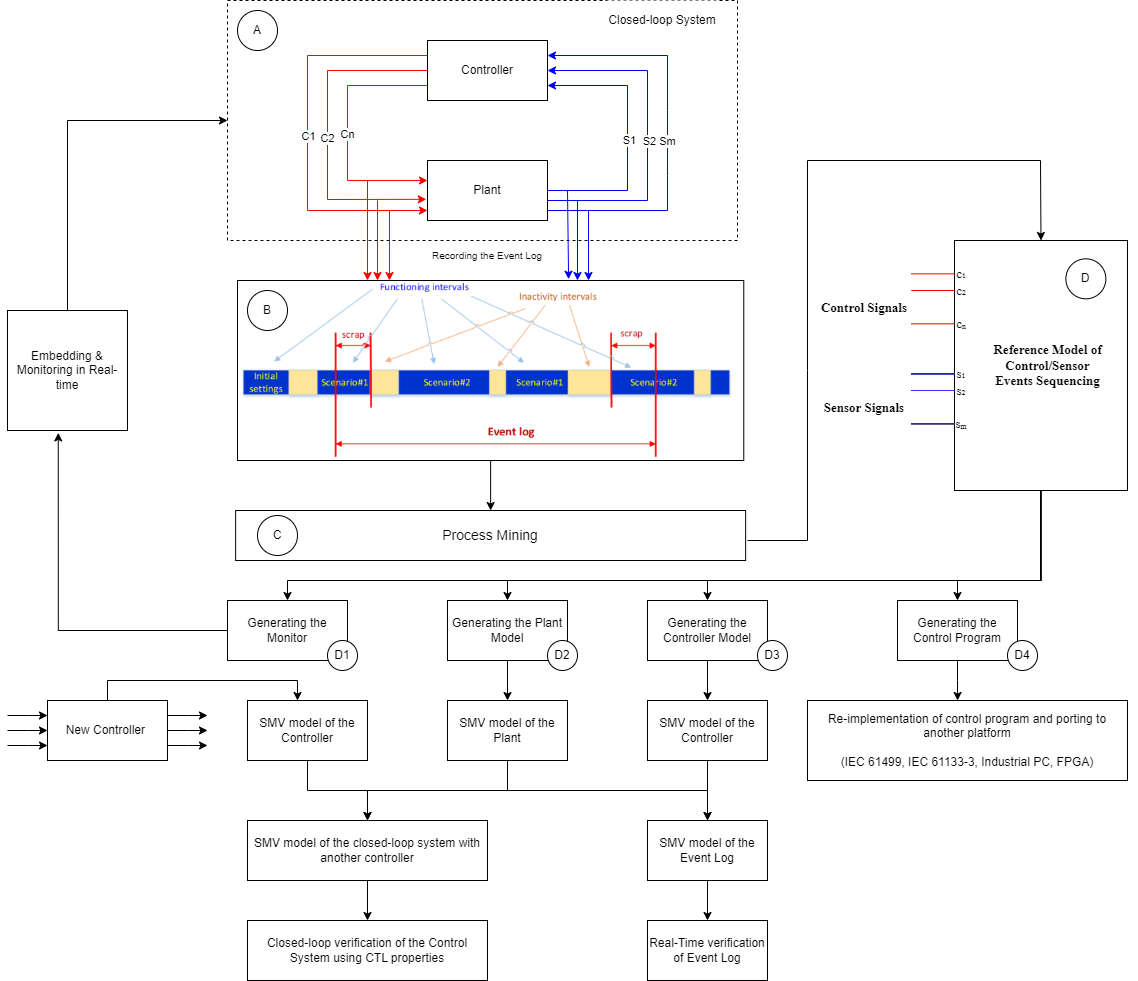
\includegraphics[width=0.9\textwidth]{MX_Papers/Paper7/images/workflow1.png}
    \caption{Workflow and use cases showing the transformation from event logs to monitor, plant model, control model, and control program}
    \label{fig:workflow_use_cases}
\end{figure}

The RMCSES interface focuses exclusively on control signals originating from the controller and informative signals originating from sensors, representing the interface between the controller and the plant. Internal signals circulating within the control system and plant are not considered, though control signals from external sources such as operators can be included. This focus on the controller-plant interface makes the model particularly suitable for closed-loop system analysis and verification.

The model assumes that each component in the system operates in a cyclical, meaningful, and locally complete manner. Components are considered to have meaningful behavior when they have specific goals and actively work toward achieving them. Each component follows specific scenarios that begin with initialization and end with termination, with multi-functional devices potentially executing different scenarios depending on their current task or operation.

\subsection{Petri Net Decomposition and State Machine Generation}

The transformation from event logs to plant models involves several sophisticated steps, beginning with Petri net construction and proceeding through decomposition and state machine generation. This process addresses the complexity of industrial systems by breaking down complex behaviors into manageable components while preserving essential behavioral characteristics.

The Petri net decomposition process utilizes reachability graph methods to identify subsets of states and transitions, facilitating the partitioning of complex Petri nets into manageable modules. This approach provides a structured and systematic method for exploring all reachable states and transitions within the system, ensuring completeness in capturing all potential behaviors.

\begin{figure}[h]
    \centering
    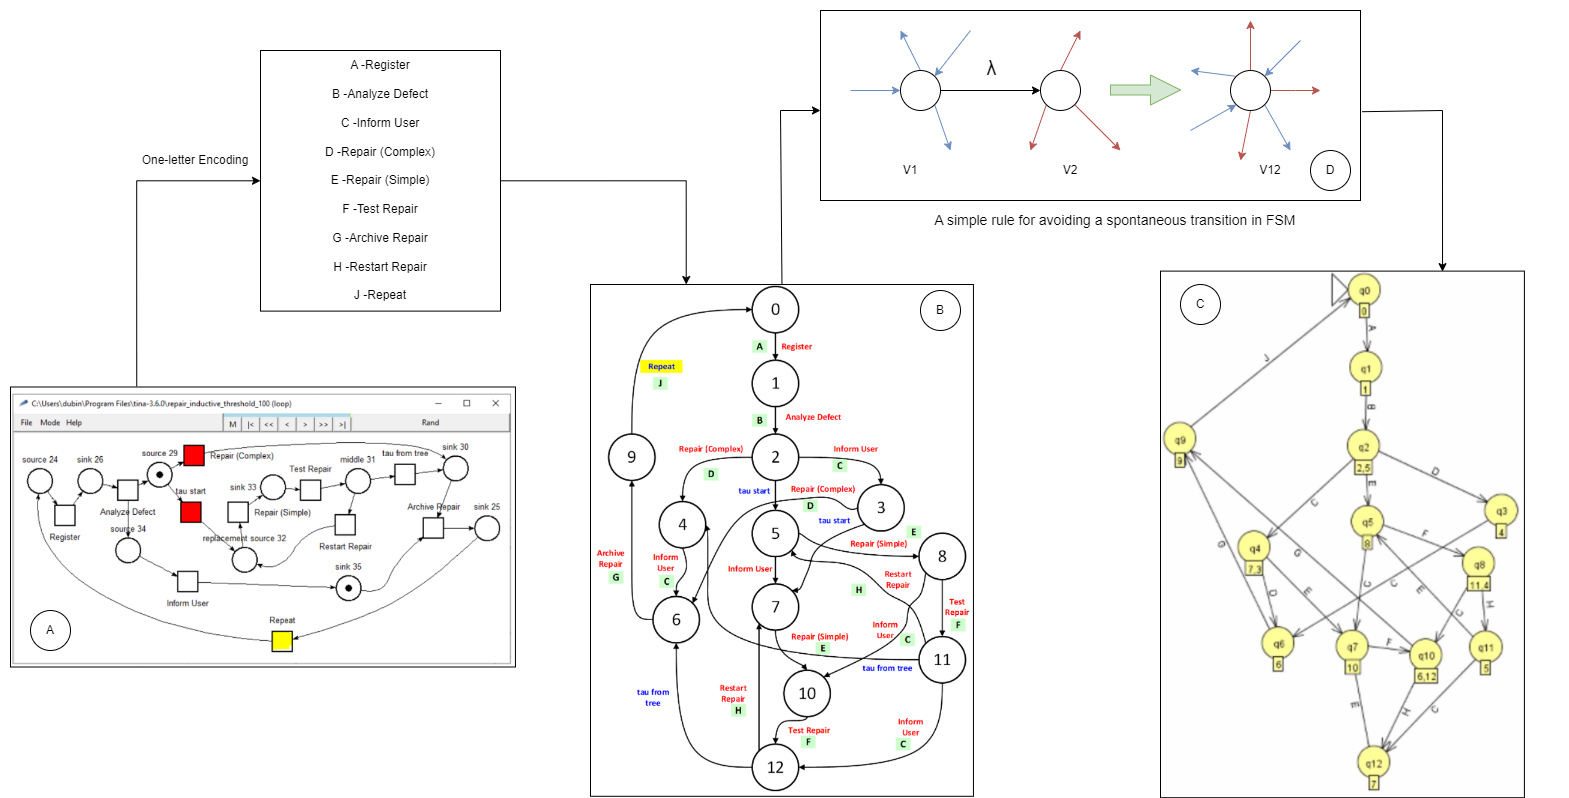
\includegraphics[width=0.8\textwidth]{MX_Papers/Paper7/images/PN2FSM.png}
    \caption{Transformation of Petri net to FSM showing the decomposition process and state machine generation}
    \label{fig:petri_net_to_fsm}
\end{figure}

The reachability graph method, while comprehensive, can suffer from state space explosion in complex systems. To address this challenge, several strategies are employed: state space reduction using symbolic representations such as Binary Decision Diagrams (BDDs), abstraction and aggregation methods that focus on essential behavioral properties, partial order reduction techniques that avoid redundant interleavings, and on-the-fly exploration that generates states as needed.

The composition of State Machine Components (SMCs) into a cohesive FSM requires careful integration to ensure synchronization and coordination. Parallel composition and synchronization techniques are preferred for IEC 61499 systems, as they align with the distributed and modular architecture of these systems. This approach enables concurrent execution of SMCs while maintaining proper coordination and communication between distributed components.

\subsection{Monitor Implementation for Real-Time Conformance Checking}

The automatic generation of monitors represents a critical application of the RMCSES, enabling real-time detection of deviations from expected system behavior. These monitors are implemented as IEC 61499 function blocks that can be deployed in operational systems to provide continuous monitoring and early warning of potential issues.

The monitor implementation involves transforming the RMCSES into a function block that receives input signals from both controller and sensor components. The monitor's ECC is generated using transformation rules that map FSM states and transitions to appropriate ECC states and transitions. When the monitor detects a valid transition, it generates an "OK" output indicating successful operation. If an unexpected event occurs, the monitor transitions to an error state and produces an "ERROR" event with details about the event that caused the error.

\begin{figure}[h]
    \centering
    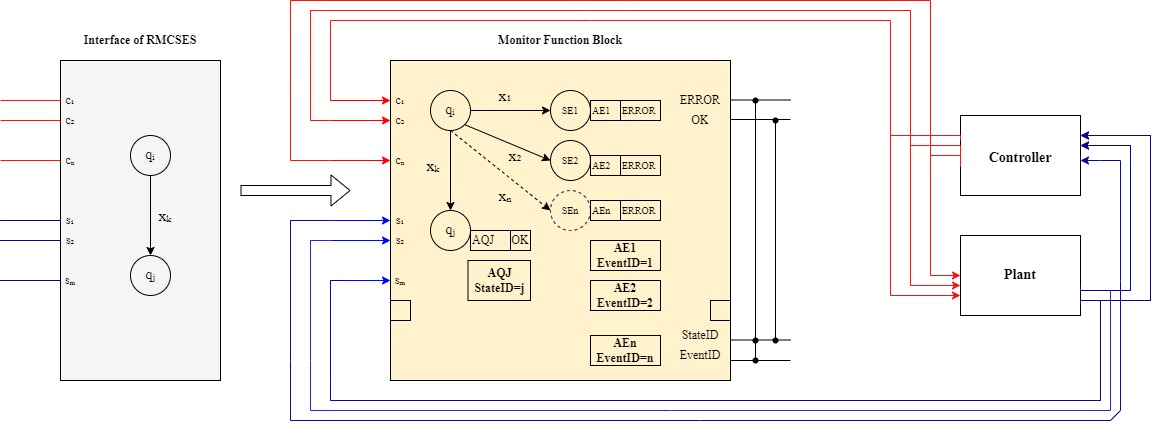
\includegraphics[width=0.9\textwidth]{MX_Papers/Paper7/images/ConformaceCheckingApp.jpg}
    \caption{Application for conformance checking showing the integration of monitor with closed-loop system}
    \label{fig:conformance_checking_app}
\end{figure}

The monitor's error detection capabilities are comprehensive, covering all possible input events from each state. For each state in the FSM, the monitor defines transitions to error states for all input events that are not specified in the reference model. This complete coverage ensures that any deviation from expected behavior is detected immediately, providing robust protection against system malfunctions and unauthorized operations.

The monitor implementation includes several important features. First, it provides detailed error information including the state where the error occurred and the specific event that caused the error. Second, it continues operation until the first error is detected, after which it becomes non-responsive to prevent further processing. Third, it can be easily integrated with existing control systems without requiring significant modifications to the operational infrastructure.

\subsection{Plant Model Generation for Formal Verification}

The automatic generation of plant models extends the capabilities of process mining to formal verification applications. These plant models represent the uncontrolled behavior of the physical system and can be integrated with control models to create complete closed-loop system representations suitable for formal analysis.

The plant model generation process involves extracting the uncontrolled plant behavior from the overall system model represented by the RMCSES. This extraction requires careful analysis to distinguish between control-driven and sensor-driven transitions, as the plant model should only respond to control signals and generate sensor signals based on its internal state.

\begin{figure}[h]
    \centering
    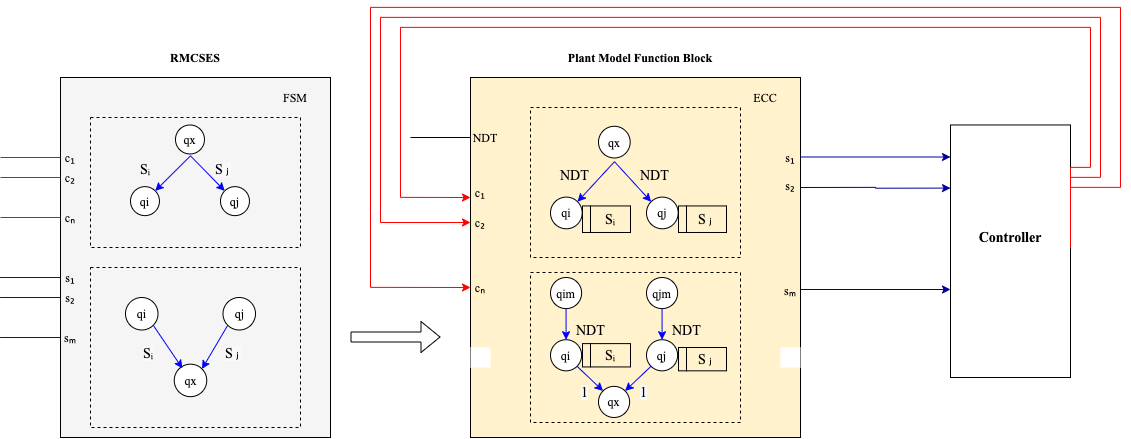
\includegraphics[width=0.9\textwidth]{MX_Papers/Paper7/images/VerificationApp1.png}
    \caption{Application for verification showing the integration of plant model with controller for formal analysis}
    \label{fig:verification_app}
\end{figure}

The transformation from FSM to plant model involves specific rules for handling sensor and control signals. Transitions triggered by sensor signals are replaced with non-deterministic transitions (NDT) that can fire at arbitrary time intervals, with the output of the next state serving as a sensor event signal. Control signal transitions remain unchanged, as the plant should respond directly to control inputs.

The plant model implementation addresses several important challenges. First, it handles diverging sensor signals by creating separate NDT transitions for each possible sensor output. Second, it manages converging sensor signals by introducing intermediate states that produce appropriate sensor signals before converging to the target state. Third, it maintains the non-deterministic nature of plant behavior while providing a deterministic interface for integration with control systems.

The generated plant model can be used for formal verification using tools such as NuSMV and CTL/LTL specifications. The model can be converted to SMV format using the fb2smv tool, enabling comprehensive analysis of system properties including safety, liveness, and reachability. This verification capability is particularly valuable for safety-critical applications where formal guarantees of system behavior are required.

\section{Integration and Applications}

The three approaches presented in this chapter represent complementary aspects of process mining applications in industrial control systems, each addressing different challenges in system understanding, control generation, and verification. Their integration provides a comprehensive framework for addressing the complex requirements of modern industrial automation.

\subsection{Comprehensive System Analysis Framework}

The integration of process model extraction, interactive learning, and automatic plant model generation creates a comprehensive framework for industrial control system analysis and development. This framework enables end-to-end system understanding, from initial behavior recording through formal verification and operational monitoring.

The framework begins with process model extraction, which provides fundamental understanding of system behavior through analysis of recorded event logs. This understanding serves as the foundation for both controller generation and plant model development, ensuring consistency across all system representations.

Interactive learning builds upon this foundation by enabling automatic controller generation from recorded behavioral traces. This approach reduces development time and improves system reliability by ensuring that control logic is consistent with observed system behavior. The generated controllers can be immediately deployed or used as starting points for further refinement.

Automatic plant model generation extends the framework to formal verification applications, enabling comprehensive analysis of closed-loop system behavior. The generated plant models can be used with existing or newly developed controllers to verify system properties and ensure compliance with safety and performance requirements.

\subsection{Industrial Applications and Case Studies}

The presented approaches have been validated through several industrial case studies, demonstrating their effectiveness in real-world applications. The gripper and conveyor system case study illustrates the application of process model extraction for system understanding and anomaly detection. This case study shows how process mining can be used to analyze complex manufacturing processes and identify potential improvements in system operation.

The interactive learning case study demonstrates the application of simulation-based controller generation for a production system with multiple components including conveyors, grippers, and autonomous guided vehicles. This case study shows how the approach can handle complex, multi-component systems and generate controllers that accurately reflect desired system behavior.

The pneumatic cylinder case study illustrates the application of automatic plant model generation and real-time monitoring. This case study shows how the approach can be used for formal verification of safety-critical systems and real-time monitoring of operational compliance.

\begin{figure}[h]
    \centering
    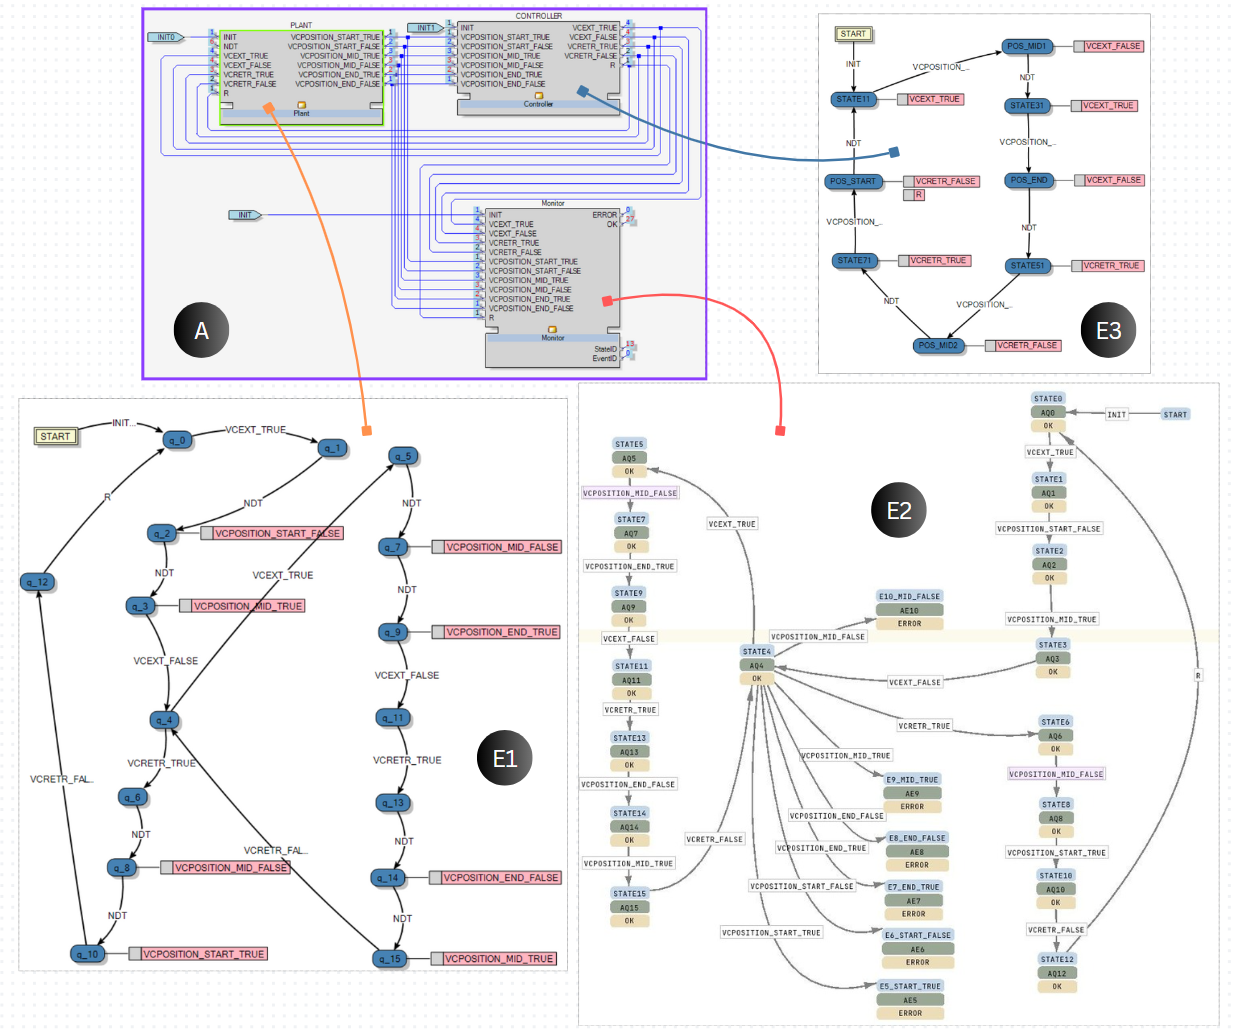
\includegraphics[width=0.8\textwidth]{MX_Papers/Paper7/images/CLMC.PNG}
    \caption{Closed-loop system integration showing plant model, controller, and monitor working together for comprehensive system analysis}
    \label{fig:closed_loop_integration}
\end{figure}

These case studies demonstrate the versatility of the presented approaches and their applicability to a wide range of industrial applications. The approaches can be adapted to different system types, from simple single-component systems to complex multi-component manufacturing lines, providing flexible solutions for various industrial automation challenges.

\subsection{Future Research Directions}

The integration of process mining with industrial control systems opens several promising research directions that could further enhance the capabilities and applicability of these approaches.

First, the development of more sophisticated process discovery algorithms could improve the quality and accuracy of generated models. Current algorithms may struggle with complex, highly concurrent systems or systems with significant noise in their event logs. Advanced algorithms that can handle these challenges would expand the applicability of the approaches to a broader range of industrial systems.

Second, the integration of machine learning techniques with process mining could enable adaptive models that improve over time based on new observations. This capability would be particularly valuable for systems that evolve or change their behavior over time, enabling continuous improvement of system understanding and control.

Third, the development of more efficient algorithms for handling large-scale event logs could enable the application of these approaches to complex, multi-facility manufacturing systems. Current approaches may face computational challenges when dealing with very large event logs or complex system architectures.

Fourth, the integration of these approaches with emerging technologies such as digital twins and edge computing could enable real-time process mining and control generation. This integration would enable dynamic adaptation of control systems based on real-time analysis of system behavior, providing more responsive and adaptive automation solutions.

The research presented in this chapter demonstrates the significant potential of process mining techniques for addressing critical challenges in industrial control systems. The three complementary approaches provide comprehensive solutions for system understanding, control generation, and verification, while the integration of these approaches creates a powerful framework for industrial automation development and analysis.

As industrial systems become increasingly complex and interconnected, the need for automated methods for system understanding and control generation will continue to grow. The approaches presented in this chapter provide a solid foundation for addressing these challenges and enable the development of more intelligent, adaptive, and reliable industrial automation systems.

The future of industrial automation lies in the integration of data-driven approaches with formal methods, creating systems that can learn from their environment, adapt to changing requirements, and provide formal guarantees of their behavior. The process mining approaches presented in this chapter represent important steps toward this vision, providing practical methods for realizing intelligent industrial automation systems that can meet the demands of modern manufacturing.


\makebib
\end{bibunit}

%%%%%%%%%%%%%%%%%%%%%%%%%%%%%%%%%%%%%%%%%%%%%%%%%%%%%%%%%%%%%%%%%%%%
%% Begin Part II - Collection of papers
%%%%%%%%%%%%%%%%%%%%%%%%%%%%%%%%%%%%%%%%%%%%%%%%%%%%%%%%%%%%%%%%%%%%

\makepartpage{Part II}%
\startpapers

% Bibliography files for papers

%-------------------------------------------------------------------
\def\paperheader{Paper A}
\def\papertitle{The Title of the Papers in the Thesis are Automatically Split In Several Lines if Necessary}
\def\paperauthorstring{John Doe and Jane Doe}
\def\referencestring{Example Thesis, Internal Report, Lule{\aa} University of Technology, 2002.}
\def\copyrightstring{2002, The Publisher, Reprinted with permission.}

% The definitions above could just as well be put directly into the function
% call below, but were explicitly defined to more clearly illustrate the
% use of the function \makepaper.

\makepaper
  {\paperheader}
  {\papertitle}
  {\paperauthorstring}
  {\referencestring}
  {\copyrightstring}

% The actual contents is imported by un-commenting the \input line below.
% Make sure the file exist.
\begin{bibunit}
\thispagestyle{plain}
\begin{center}
\Large\textbf{The Tile of the Paper}\\
\vspace{10mm}
\normalsize John Doe and Jane Doe\\
\vspace{15mm}
\textbf{Abstract}\\
\end{center}
Abstract text of the paper...

\section{Introduction}
The text of this article is imported from the file
\textit{paper1.tex}. The title and abstract part above are typeset
manually (see file for code template).
\cite{Goossens}

\acrfull{nlp} is the full version of this short version \acrshort{nlp} and the long version \acrlong{nlp}. 

Be sure NOT to have any $\backslash$begin\{document\} or
$\backslash$end\{document\} tags in the imported files.

Some references here too, just to show the use of bibunits
\nocite{*}.

\paperappendix
\section{First appendix of paper A}
Some appendix text.
\subsection{A subsection of the appendix}
%
\begin{equation}
    X(\omega) = \int_{-\infty}^{\infty} x(t)e^{-j\omega t}\,dt.
\end{equation}
%
\subsection{Another subsection of the appendix}
\subsubsection{Test subsubsection}

\section{Another appendix}
Some text in the second appendix

%%% Put references here
\putbib
\end{bibunit}



%-------------------------------------------------------------------
\def\paperheader{Paper B}
\def\papertitle{Cyber-physical automation systems modelling with IEC 61499 for their formal verification}
\def\paperauthorstring{Midhun Xavier, Sandeep Patil, Valeriy Vyatkin}
\def\referencestring{Proceedings of the IEEE International Conference on Industrial Informatics (INDIN), 2021.}
\def\copyrightstring{2021, IEEE, Reprinted with permission.}

% The definitions above could just as well be put directly into the function
% call below, but were explicitly defined to more clearly illustrate the
% use of the function \makepaper.

\makepaperaccepted
  {\paperheader}
  {\papertitle}
  {\paperauthorstring}
  {\referencestring}
  {\copyrightstring}

% The actual contents is imported by un-commenting the \input line below.
% Make sure the file exist.
\begin{bibunit}
\thispagestyle{plain}

% Add missing command definitions from original paper
\newcommand \op[1] {\ensuremath{\operatorname{\mathbf{#1}}}}
\newcommand \com[1] {\ensuremath{\mathtt{#1}}}
\newcommand{\RNum}[1]{\uppercase\expandafter{\romannumeral #1\relax}}

\section{Introduction}

Distributed industrial automation systems pose a significant challenge for their efficient verification and validation due to their heterogeneous structure, use of wireless communication and decentralised logic. The inherent inter twinning of computational and communication processes with complex physical dynamics has called for the term cyber-physical systems (CPS) \cite{lee2017introduction} to emphasize the challenges and the need for new development approaches.   

The {IEC 61499} architecture \cite{iec61499part12012} is getting increasingly recognised as a powerful mechanism for engineering such systems. 
It has been proven also as an efficient way of modeling CPS in automation \cite{dai2017discrete}. 

The challenge of IEC 61499 verification has been well-recognized from the early stages of the standard's development and evaluation \cite{vyatkin1999modeling}. Closed-loop modelling has been proposed for the most comprehensive verification \cite{vyatkin2008closed}, which implies the need for modelling the plant. 

In quite many works, the plant modelling \cite{buzhinsky2016plant} was done in the same formalism, which was used eventually to represent the model for the model-checker. Graphical modelling languages of finite-state machines and Petri nets \cite{berthomieu1991modeling} were used in particular, and the models were prepared using the corresponding graphical editors.
However, the IEC 61499 itself provides a graphical engineering interface and supports programming in terms of state machines. Therefore, a problem-oriented notation could be proposed to take advantage of the existing tools and avoid using additional ones in the process of modelling. This paper proposes such an approach by introducing a tool chain.

%Industrial automation has been around for many decades. The field is vastly explored and today’s cyber-physical systems (CPS) are very intricate and complex. Designing such automated cyber-physical systems are challenging. With the increased complexity of the distributed automation systems,  it is  natural  that the  frequency  or  magnitude  of  issues  increases as  well. It is important to identify the problems in the system. Formal model computation offers a solution to this by evaluating a model of a plant in regards to the functional properties of the CPSs.  An interesting field to explore is if we can generate  a tool chain which completely implements, simulates, verifies and analyzes the distributed CPSs. 

%We introduced a tool chain which helps to completely develop, analyze and test the whole system. The tool chain consists of several tools. The tool chain is helpful to detect the error, fix the issue and test again. The developers working on complex designs of automated CPSs can use this tool effectively for continuous development to implement fault free systems. In this paper we use mainly FB2SMV, NuSMV and Nutrac tools: The FB2SMV which creates the formal model of the automated CPSs, NuSMV is used to simulate and verify the specification of the formal model, and finally Nutrac creates better view of counter example. 

The paper is structured as follows: Section \RNum{2} discusses the related work and problem statement. Section \RNum{3} and \RNum{4} illustrates an example and  simulation model in detail. Section \RNum{5}  describes the discrete-state modelling approach including the implementation of non-deterministic transition in smv. Section \RNum{6}  gives an overview of the fb2smv tool's functionalities and features. Section \RNum{7}  presents the results and analysis of the work. Finally, Section \RNum{8} concludes the paper and outlines future goals.


\section{Related works and problem statement}

Christensen suggested a model-driven development approach \cite{christensen2000design} for distributed automation systems that is based on the use of the model-view-control object-oriented design pattern. The approach supports several development stages, from simulation in the loop to the deployment~\cite{patil2018adapting}. 
In \cite{vyatkin2008closed} that approach was extended to also include formal verification into the verification and validation of function block systems.

The suggested framework is heavily based on the closed-loop architecture of the model, where the plant part is explicitly represented in the overall system model. This architecture allows for easy integration with a simulation model for the virtual commissioning purposes, which can be seamlessly converted to the deployment configuration. In addition, the closed-loop configuration could be transformed to a structurally similar formal model, appropriate for more exhaustive verification by means of model-checking.   
The concept of an integrated environment VEDA presented in \cite{vyatkin2003verification} had already supported closed-loop verification of IEC 61499 function block systems. While the controller parts of the closed-loop models were automatically translated into the corresponding formal model in a Petri-net like language, the model of the plant parts had to be developed manually in the same formalism. 
This made the process of model creation quite difficult, not allowing for systematic use of the tool by control engineers. 
The emergence of the automatic model generator fb2smv \cite{fb2smv} that is capable of creating SMV models from IEC 61499 function block systems, promises increased potential of formal verification on account of using the industry grade model-checkers of the NuSMV \cite{cimatti2000nusmv} and NuXMV family. 
However, the problem of creating the model of plant in SMV remains to be the limiting factor~\cite{sinha2019survey} for industrial application of the corresponding verification tool-chain.

In this paper, we attempt to overcome this hurdle by proposing a CPS modelling method that is entirely based on IEC 61499. By means of the same modelling language, we represent both simulation models of the plant, which are equivalent to hybrid automata, and the models for formal verification, which are equivalent to discrete-state automata with non-determinism. 
The latter model can be derived from the former by applying a sequence of transformation steps. 

Both kinds of plant models, implemented as IEC 61499 function blocks can be included in the multi-closed-loop model connected to the real controllers. This opens the opportunity of checking the distributed control logic of CPS in simulation and model-checking.  

\section{Illustrative example}

The modelling method and tool-chain used for CPS verification are illustrated in this paper using a laboratory-scale distributed automation system "Drilling station", described in the next subsection. In this case study, we selected and created a formal model for the same system. Implementation of formal models of real systems as well as verification is done with the help of the tool chain. 

%The tool chain discusses the accurate implementation of plant models and controllers with the help of Non Deterministic Transitions (NDTs) in nxtStudio and FBME environment, FB2SMV tool which creates of formal models by converting function blocks to SMV code, NuSMV tool helps to simulate and verify by checking various CTL specifications and Nutrac tool for better representation of counter-example in CSV format.


\begin{figure}
    \centering
    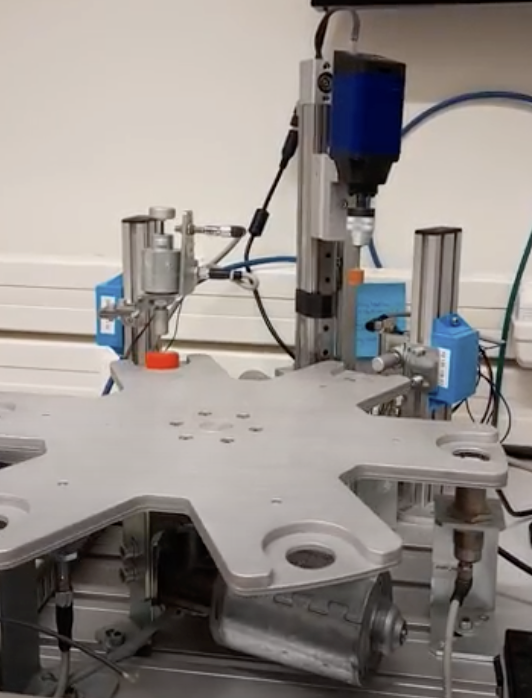
\includegraphics[scale = 0.2]{MX_Papers/Paper2/images/DT_REAL.png}
    \caption{Drilling station system.}
    \label{figure:RealImageofDrillTable}
\end{figure}

%\subsection{Demonstrator description}

The drilling station system in Fig. \ref{figure:RealImageofDrillTable} is composed of several mechatronic components, among which, in this study we selected only the Drill and rotating Table. 
It is assumed that the mechatronic components are smart, i.e. they are equipped with their own control devices, implementing their basic operations, which are as follows. 

The Drill moves in an upward or downward direction. Whenever a workpiece is detected by the sensor under the drill, it moves downward and starts drilling. Once it completes drilling, it moves upwards and rests at the home position. 

The Table rotates from one fixed position to another. The cycle is completed when it rotates six times. 
When a workpiece is placed in the loading positions, the table rotates to bring it under the drill.

The control logic of each mechatronic component is implemented as a function block which follows the IEC 61499 standard. The function block diagram  shown in Fig. \ref{figure:RealFBDiagram} consists of the two function blocks orchestrated to work together by means of event and data connections between each other and sources and sinks of sensor inputs and actuator outputs (function blocks on the left hand side and right hand side respectively). A close-up on the interacting controllers is presented in Fig. \ref{figure:RealFBControllers}.

It is assumed that the smart mechatronic components are delivered by their vendors together with the software components for implementing their control logic. They are integrated to the drilling station in a way, assuming that the control of internal operations in each mechatronic component is implemented by its predefined function block, and the integrator tries to minimise its software development effort by reusing the software components received from the vendors.
This approach requires exhaustive testing of the orchestrated system on compliance with functional and non-functional requirements. 

Hence, we will use both simulation in the loop with the plant model and formal verification in closed loop for more exhaustive exploration of the state space. 



\begin{figure}
    \centering
    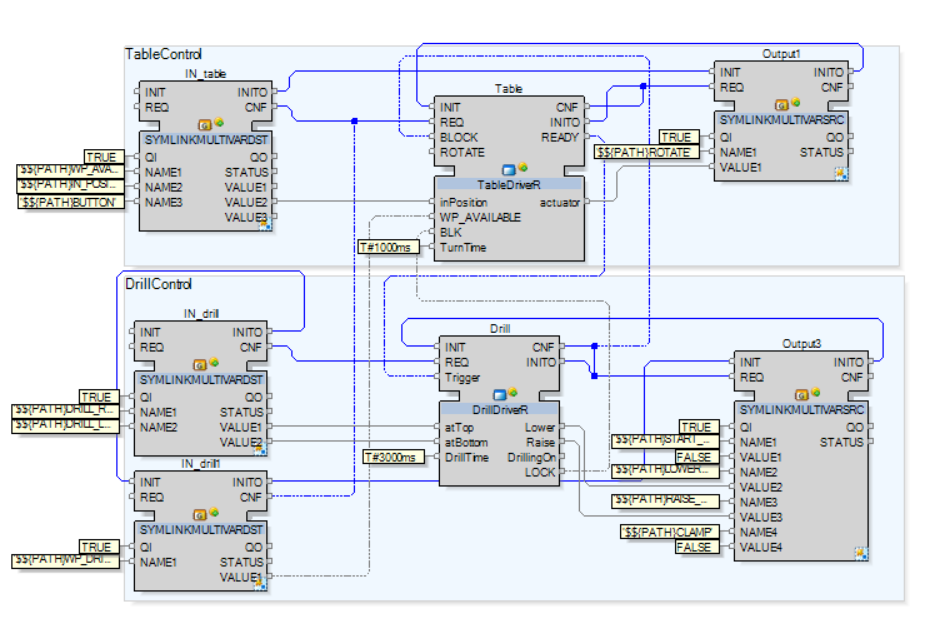
\includegraphics[scale = 0.4]{MX_Papers/Paper2/images/fig2updated.PNG}
    \caption{Function block representation of the distributed automation of drilling station.}
    \label{figure:RealFBDiagram}
\end{figure}

\begin{figure}
    \centering
    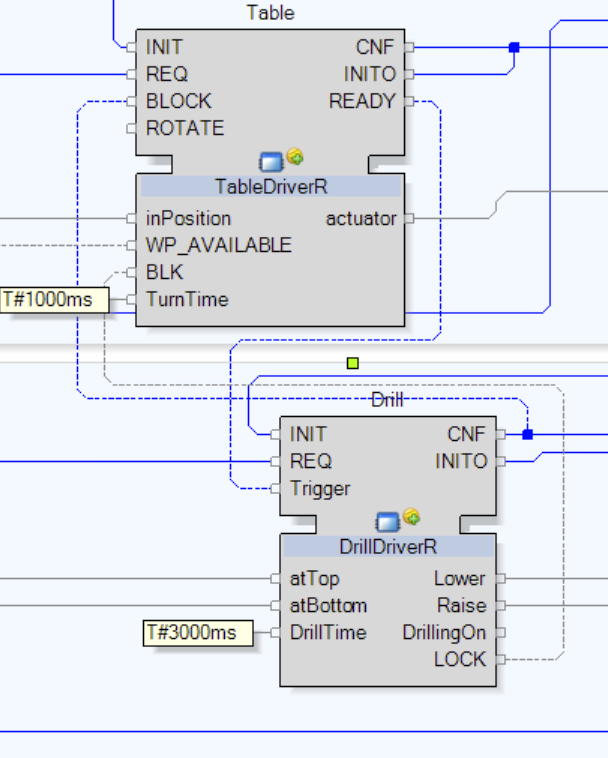
\includegraphics[scale = 0.20]{MX_Papers/Paper2/images/DT_REAL_FB_CONTROLLERS.png}
    \caption{Close-up on the decentralised controllers' interaction.}
    \label{figure:RealFBControllers}
\end{figure}

\section{Simulation Model}

The simulation-in-the-loop environment is shown in Fig. \ref{figure:SimulationFBDiagram}.  The original  function blocks containing the autonomous control logic of drill and table are connected with the function blocks implementing simulation models of the drill and table respectively. The controllers are also connected with each other in exactly the same way as in the real configuration in Fig. \ref{figure:RealFBControllers}. 
For example, the function block TableMod11 of type TableModTop represents a model of the table that is driven by one control signal \com{fwd}. When this signal receives the value \com{TRUE}, the simulated table starts continuous rotation clockwise. The rotation is stopped if \com{fwd} resets to \com{FALSE}.

The model outputs the Boolean value \com{FixPos} which becomes \com{TRUE} when the table comes to one of the six fixed positions. To keep the table in the fixed position, the controller has to stop motion by resetting the control signal \com{fwd} to \com{FALSE}. Besides, the model produces the \com{WP\_DRILL} signal, which is the reading from the sensor indicating the presence of a workpiece under the drill.

The simulation environment reproduces the working behavior of the real plant which helps to visually identify the behavior of the system before deploying the distributed control to the real hardware. Besides, the errors identified during the formal verification can be represented in simulation. 

\begin{figure}
    \centering
    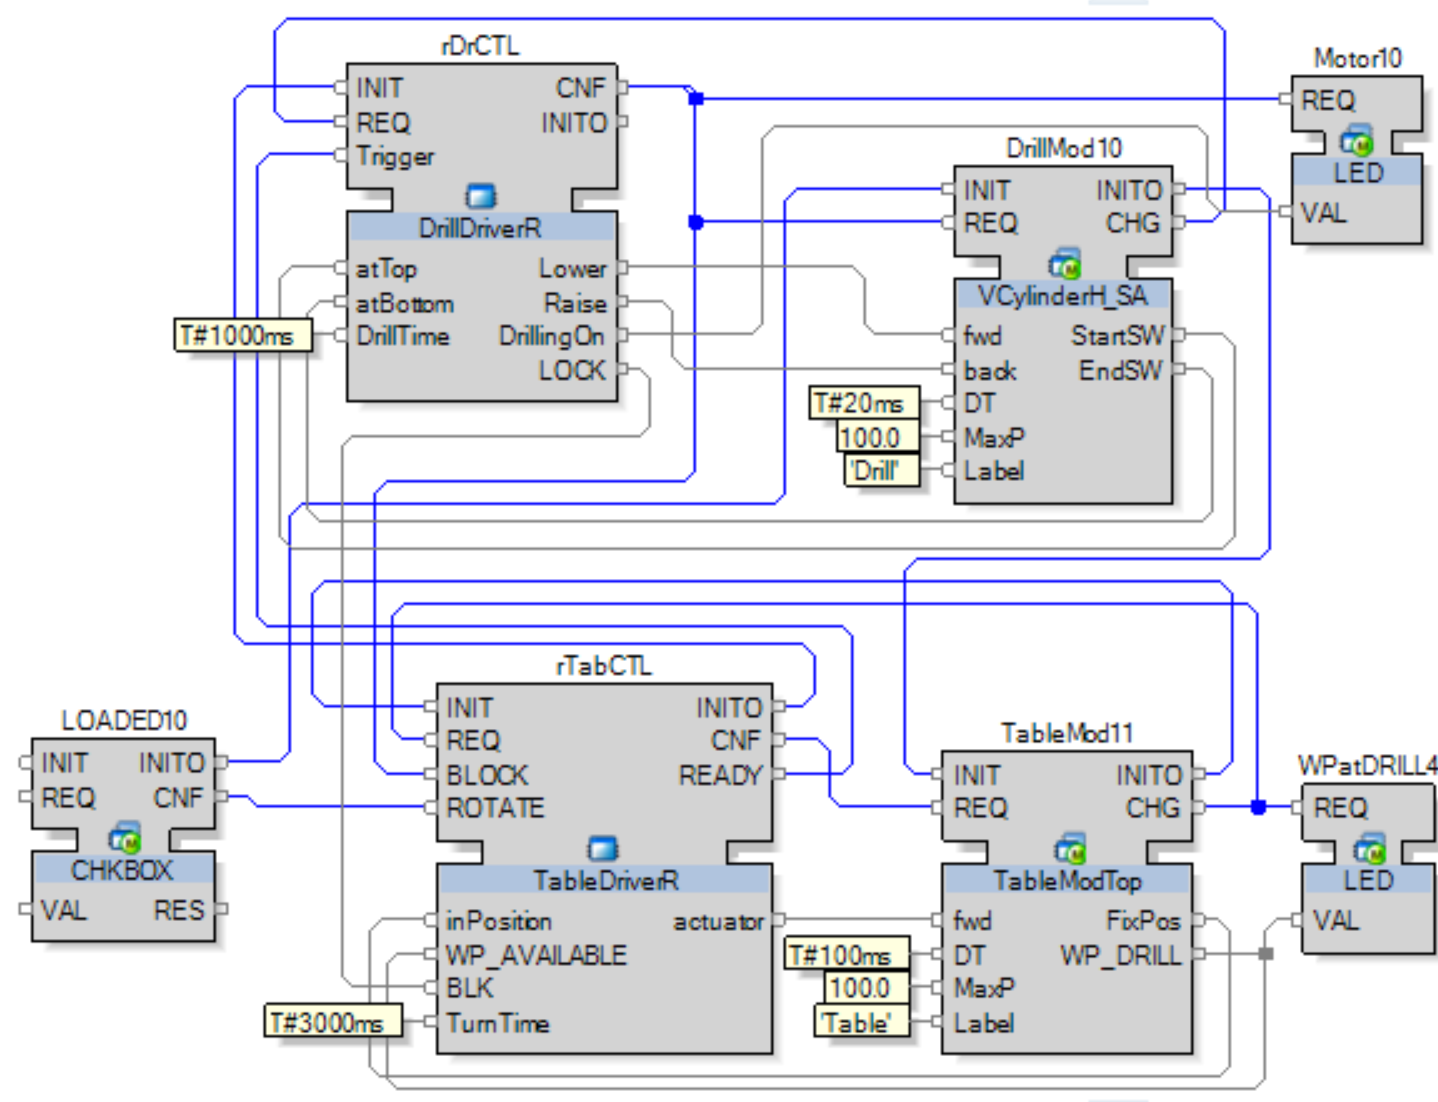
\includegraphics[scale = 0.3]{MX_Papers/Paper2/images/SimulationFBsystem.png}
    \caption{The Function Block representation of the  simulation-in-the-loop configuration.}
    \label{figure:SimulationFBDiagram}
\end{figure} 



The simulation models, used in this configuration, have continuous dynamics, which is the time-domain implementation of hybrid state machine as discussed in \cite{vyatkin2008closed}. 
The core part of the plant simulation function block is based on the hybrid automaton model of the process, as illustrated in Fig. \ref{figure:Hybrid}.
The state machine has three states corresponding to the static position of the moving object, such as the vertical axis of the drill, or the rotating table. These are {stHOME}, {stEND} and {stSTOP}. There are also two dynamic states, when the coordinate of the object is changing: {dMOVETO} and {dRETURN}. 

When the state machine is in the one of the dynamic states (say, {dMOVETO}), it emits the START output event which invokes the external {E\_CYCLE} FB, which starts emitting periodic events, activating the function block with the state machine. 
The state machine remains in the {dMOVETO} state until the position reaches the end position, i.e. Pos=DIST. Until then the loopback transition condition is true, so the state-machine remains in the {dMOVETO} state. Every time the loopback transition is executed, the event CHG is emitted which also invokes the external "Integrator" FB, which recalculates the new value of the process variable based on the current value. The duration of the time interval between recalculations is determined by the {DT} parameter of the {E\_CYCLE} and speed of the motion. 

\begin{figure}
    \centering
    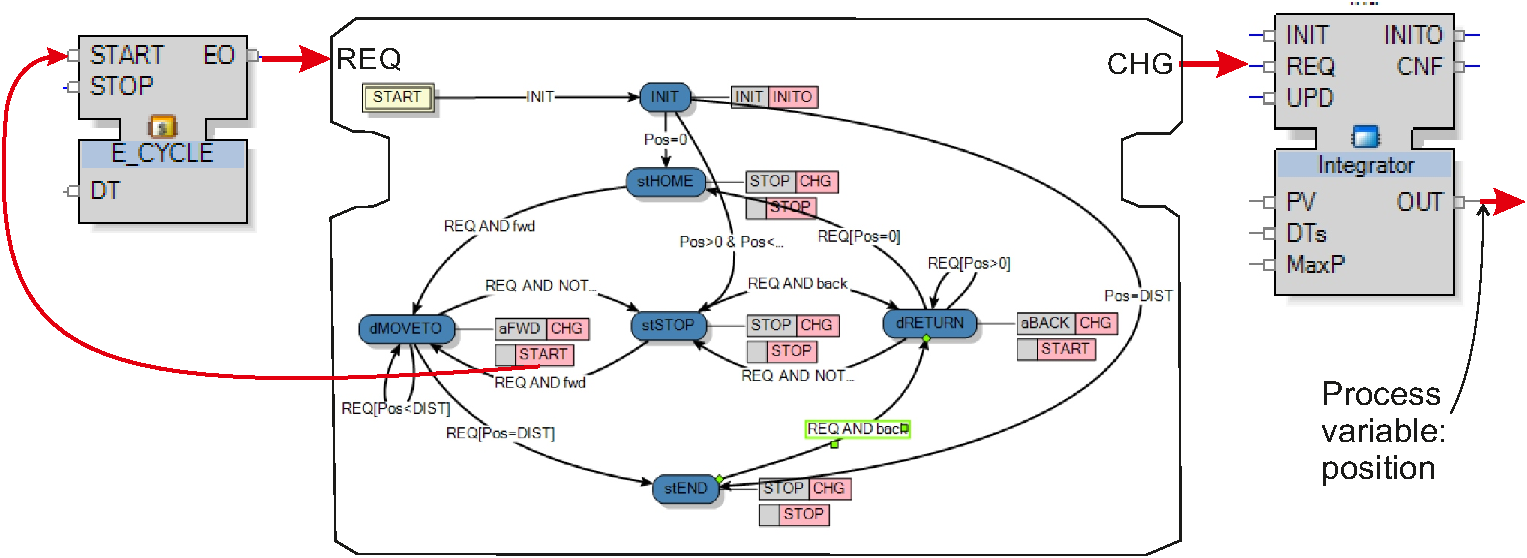
\includegraphics[scale = 0.36]{MX_Papers/Paper2/images/hybrid.pdf}
    \caption{Computational implementation of a hybrid automaton in function block.}
    \label{figure:Hybrid}
\end{figure}

Given the ever changing process values, the evolution of the model can be visually displayed using internal or external means. The development reported in this paper was done using the NxtStudio of NxtControl, which offers a proprietary visualisation technology called {CAT}. The plant model blocks were implemented as the {CATs}, therefore the model behaviour was implemented internally, within the same development environment. The interactive system visualisation by means of CATs is shown in Fig. \ref{figure:SimulationDiagram}.

\begin{figure}
    \centering
    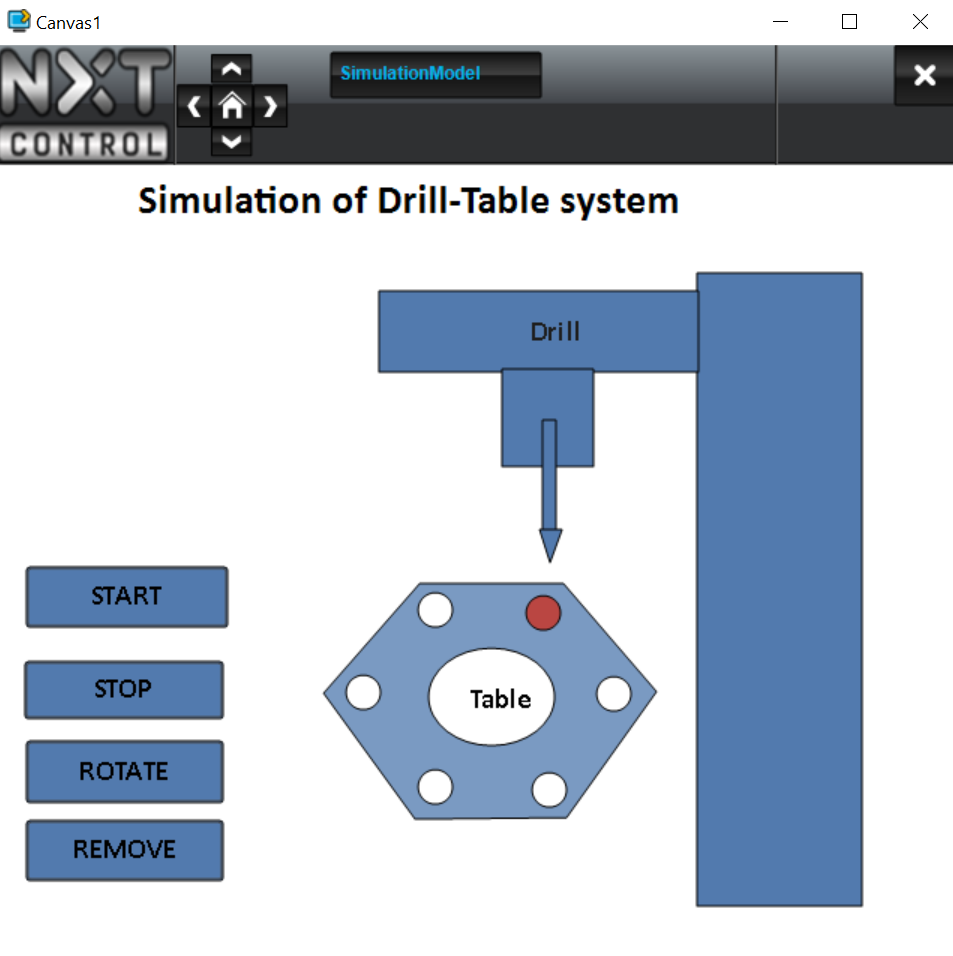
\includegraphics[scale = 0.30]{MX_Papers/Paper2/images/DT_HMI5.PNG}
    \caption{The visual representation of the simulation process.}
    \label{figure:SimulationDiagram}
\end{figure}

\section{Discrete-state Modelling Approach}

The discrete-state model of the system is created in IEC 61499 based on the simulation model described in the previous section. 

%The real system should be modeled for the verification so that the desired behavior of the system can be simulated and verified, prior to the installation of the system in real. Accurate plant modelling is necessary to identify the errors in the system. By introducing the Non deterministic transition concept in the function blocks makes the system behaviour similar to real systems.

%In order to do formal verification of the system,  we may need to modify the model of the plant to a simpler one by eliminating other features i.e. like HMI. Discrete state plant modelling in function blocks is implemented to verify the specification using SMV. Discrete state plant modelling in function blocks and followed by modelling of non-determinism in SMV can be used to identify the possible flaws in the system.

%\subsection{Discrete State Plant Modelling in Function Blocks with Non-deterministic Transitions}

%The system consists of the Drill section and Table section. First we model the drill part, but in order to  convert the function block to smv code we need to eliminate features used for visualization. In this paper, we implement a simple function block which consists of the desired behavior of the drill section of the actual system. In simulation we used the function block (shown in figure \ref{figure:SimulationFBController}) for the drill model. 


%\begin{figure}
%    \centering
%5    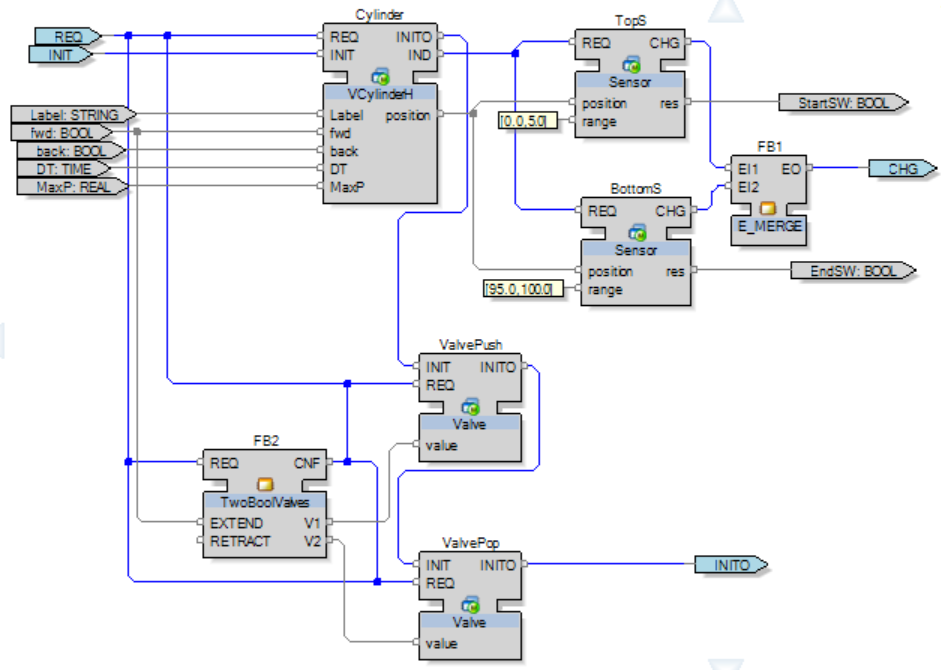
\includegraphics[scale = 0.40]{MX_Papers/Paper2/images/DrillController_sim.png}
%    \caption{The Function Block representation of Drill controller in Simulation model}
%    \label{figure:SimulationFBController}
%\end{figure}


%\begin{figure}
%    \centering
 %   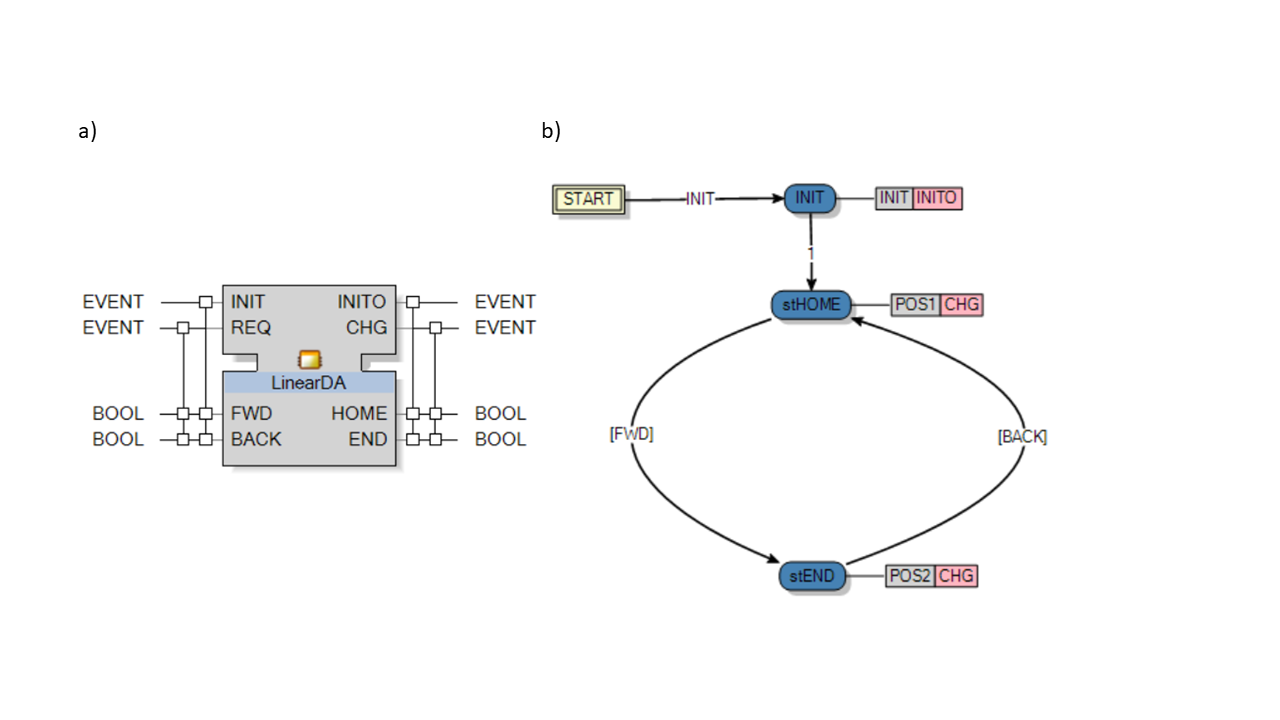
\includegraphics[scale = 0.30]{MX_Papers/Paper2/images/DrillInterfaceECC_withoutNDT.png}
%    \caption{a) The FB interface of discretized Drill model b) The ECC representation of discretized Drill model}
%    \label{figure:DrillDiscreteInterfaceECC}
%\end{figure}

The discrete-state equivalent of the simulation configuration is shown in Fig. \ref{figure:FBver}. Here the function blocks simulating the drill and table are substituted by their analogs operating in the discrete state domain, instead of modelling the continuous process parameters, such as the drill's and table's numeric position.
The model can be then simulated in the IEC 61499 IDE with values of function block inputs and outputs displayed and modified interactively. It can be translated to the SMV model using the fb2smv tool and exposed to the formal verification by model-checking. 


%This complex model can be simplified by discretizing the plant model function block to a simple meaningful one without losing its functionality. Interface is given in the figure \ref{figure:DrillDiscreteInterfaceECC} a) but it is a simple basic function block with the functionality of a drill model. The execution control chart is shown in figure \ref{figure:DrillDiscreteInterfaceECC} b) has stHOME and stEND states. Depending on the FWD and BACK signal drill model moves from one state to another but behavior of the system is straight-forward and it fails to identify the critical flaws in the system. In actual systems, drill does not come directly from stHOME to stEND state or vice versa, it might take some amount of time. In our current execution control chart, drill is suddenly moved from stHOME/stEND to stEND/stHOME. Introducing non-deterministic transitions helps to implement a similar model of plant with less complexity. The following section describes plant modelling with NDTs.



\subsection{Notation for Plant Modelling}

%It is a basic function block with standard interface consist of INIT, REQ and NDT event inputs and INITO and CHG event outputs. All data inputs are associated with INIT and REQ event inputs likewise all data outputs are connected with INITO and CHG event outputs. The figure \ref{figure:DrillNDTInterfaceECC} a) which shows a function block interface of the drill model. The NDT event is used in the execution control chart where non-deterministic choice is required.  We introduced the motion states  to achieve the unknown duration from fixed states to motion states with the help of NDT signal. 

\begin{figure}
    \centering
    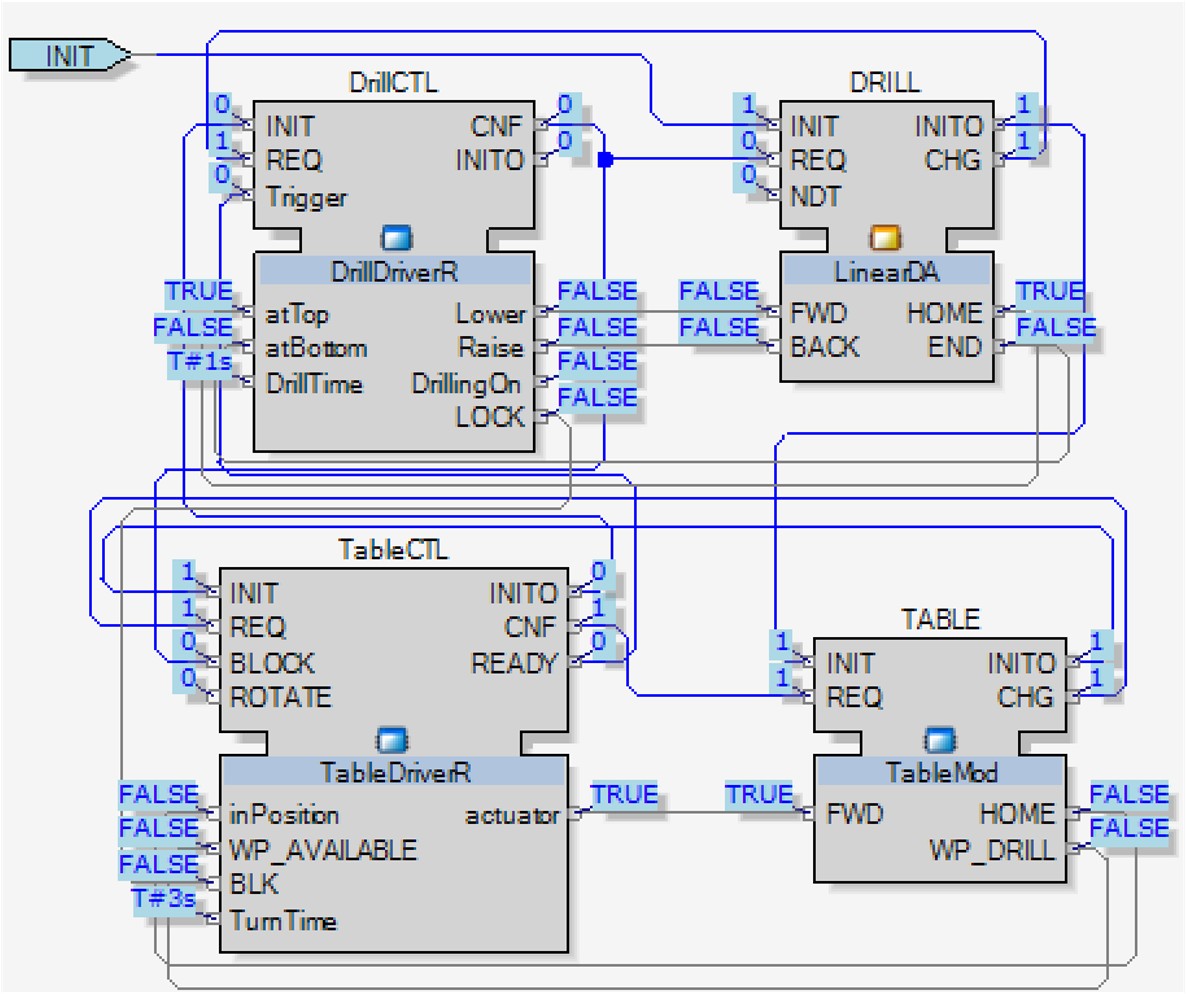
\includegraphics[scale = 0.65]{MX_Papers/Paper2/images/VerificationFB.png}
    \caption{Discrete state function block model of the Drilling station. }
    \label{figure:FBver}
\end{figure}

In the current example, the drill model is represented by an instance of a basic discrete motion model LinearDA. 
Its state-machine implementation is shown in Fig. \ref{figure:DrillECC}. The execution semantics of the state-machine follows the rules of IEC 61499, i.e. the function block is activated by an input event, and the state machine evolution is following the rules for execution control chart (ECC) of basic function blocks. 

Similarly to the hybrid state-machine in Fig. \ref{figure:Hybrid}, the discrete state model of the drill specifies  three static and two dynamic states, but it does not model the position as a numeric value. The drill moves from {stHOME} to {stEND} state via a motion state called {ddMOVETO}. The state transition occurs from stHOME to ddMOVETO whenever FWD signal is TRUE. 
It is remarkable to note the NDT event input of the LinearDA function block, which remained unassigned in the application in Fig.\ref{figure:FBver}.
The NDT is reserved in the proposed modelling notation for Non-Deterministic Transition. 
Whenever the formal model generator encounters NDT in the state machine, it will interpret it accordingly. For example, the SMV modelling of NDT will be described in section \ref{sec:NDTinSMV} 

In terms of our model, the use of NDT in the transition from the motion state {ddMOVETO} to the static state {stEND} models the unknown duration of the motion from one state to another. Plant may fail whenever the {FWD} and {BACK} signals become {TRUE} simultaneously, so we introduced an ERROR state which helps to identify whether the controller creates this scenario.

%Unknown duration from one fixed state to another can be implemented with help of motion state and modelling of non-determinism in SMV. we need to provide the signal to choose different values in each transition. SMV provides a way to accomplish non-deterministic choice by providing a set of values to the signal.


\begin{figure}
    \centering
    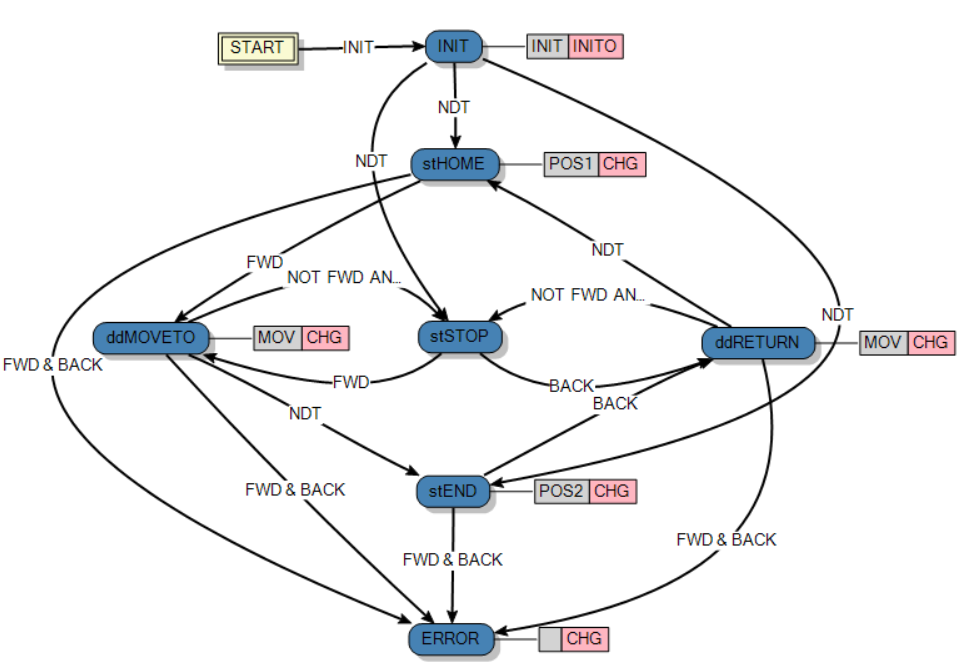
\includegraphics[scale = 0.4]{MX_Papers/Paper2/images/LinearDAFinal.PNG}
    \caption{Discrete state linear motion process model with NDT. }
    \label{figure:DrillECC}
\end{figure}


\subsection{Non Deterministic Transitions in controllers}

Non-deterministic transition can be also helpful for simplification of controller models containing timers. For example, in our case study, the controllers were developed as state machines with timeouts, therefore they are implemented in composite function blocks. In the drill, drilling process needs to be done for several durations, which is achieved  with the help of The E\_DELAY function block. The composite function block consists of a real controller and E\_DELAY function block as shown in Fig. \ref{figure:DrillInterfaceControllers}(a). 

\begin{figure}
    \centering
    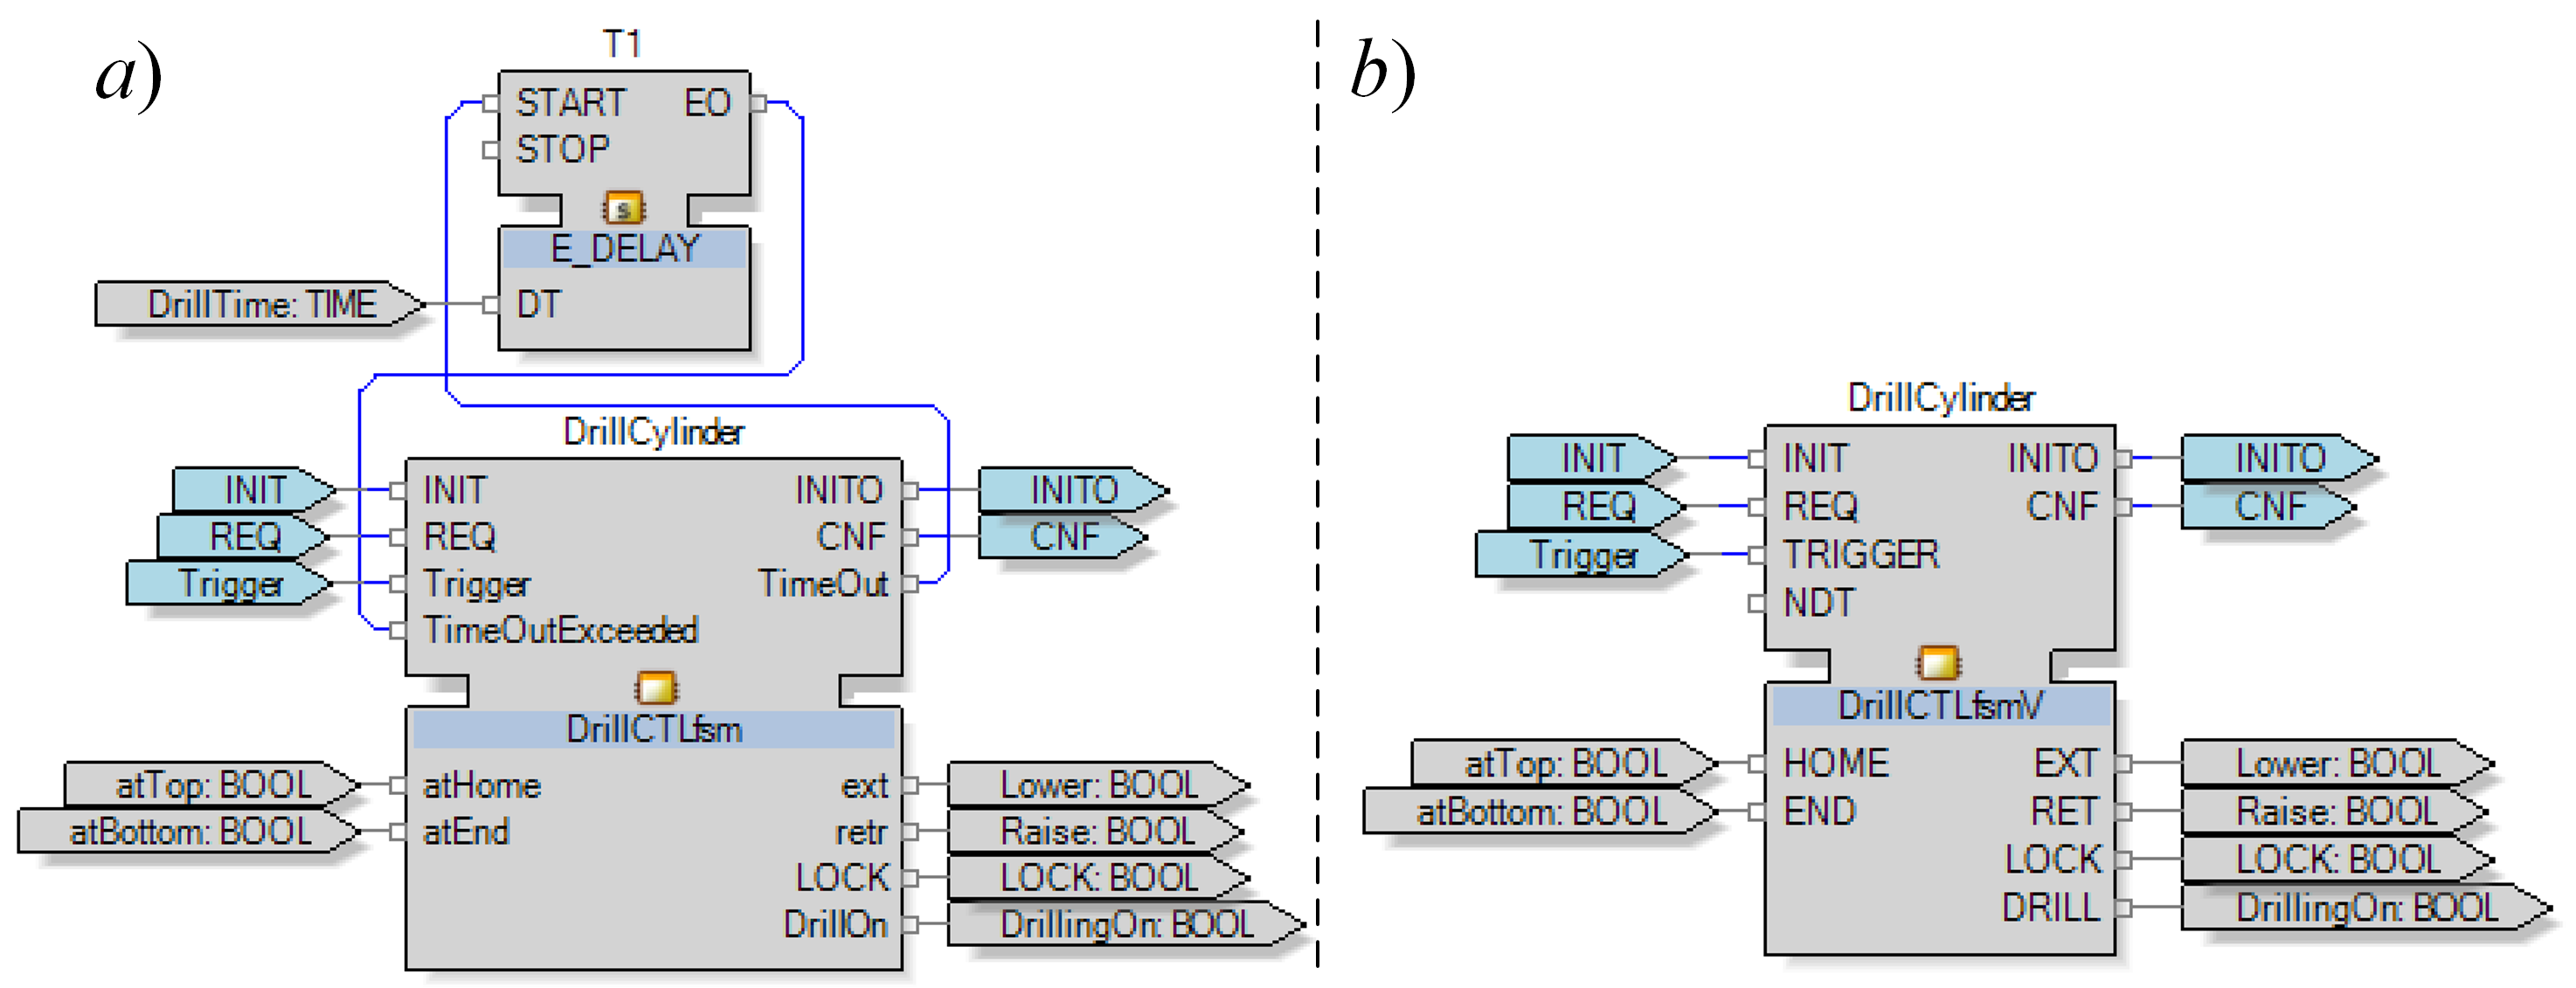
\includegraphics[scale = 0.33]{MX_Papers/Paper2/images/Fig9.png}
    \caption{ a) The real drill controller with external timeout. b) The interface of modified drill Controller with non- deterministic transition input.}
    \label{figure:DrillInterfaceControllers}
\end{figure}

However, formal modelling of the timers in SMV is computationally hard. It can be avoided if the concrete delay duration was substituted by non-deterministic transitions with the help of NDT signal. Therefore, the controllers can be modified this way in order to reduce complexity of model-checking. Therefore, we removed the timeout E\_DELAY substituted the corresponding input of the function  block and added NDT input. The execution control chart of the real drill controller and the modified drill controller are shown in Fig. \ref{figure:DrillECCControllers}.

\begin{figure}
    \centering
    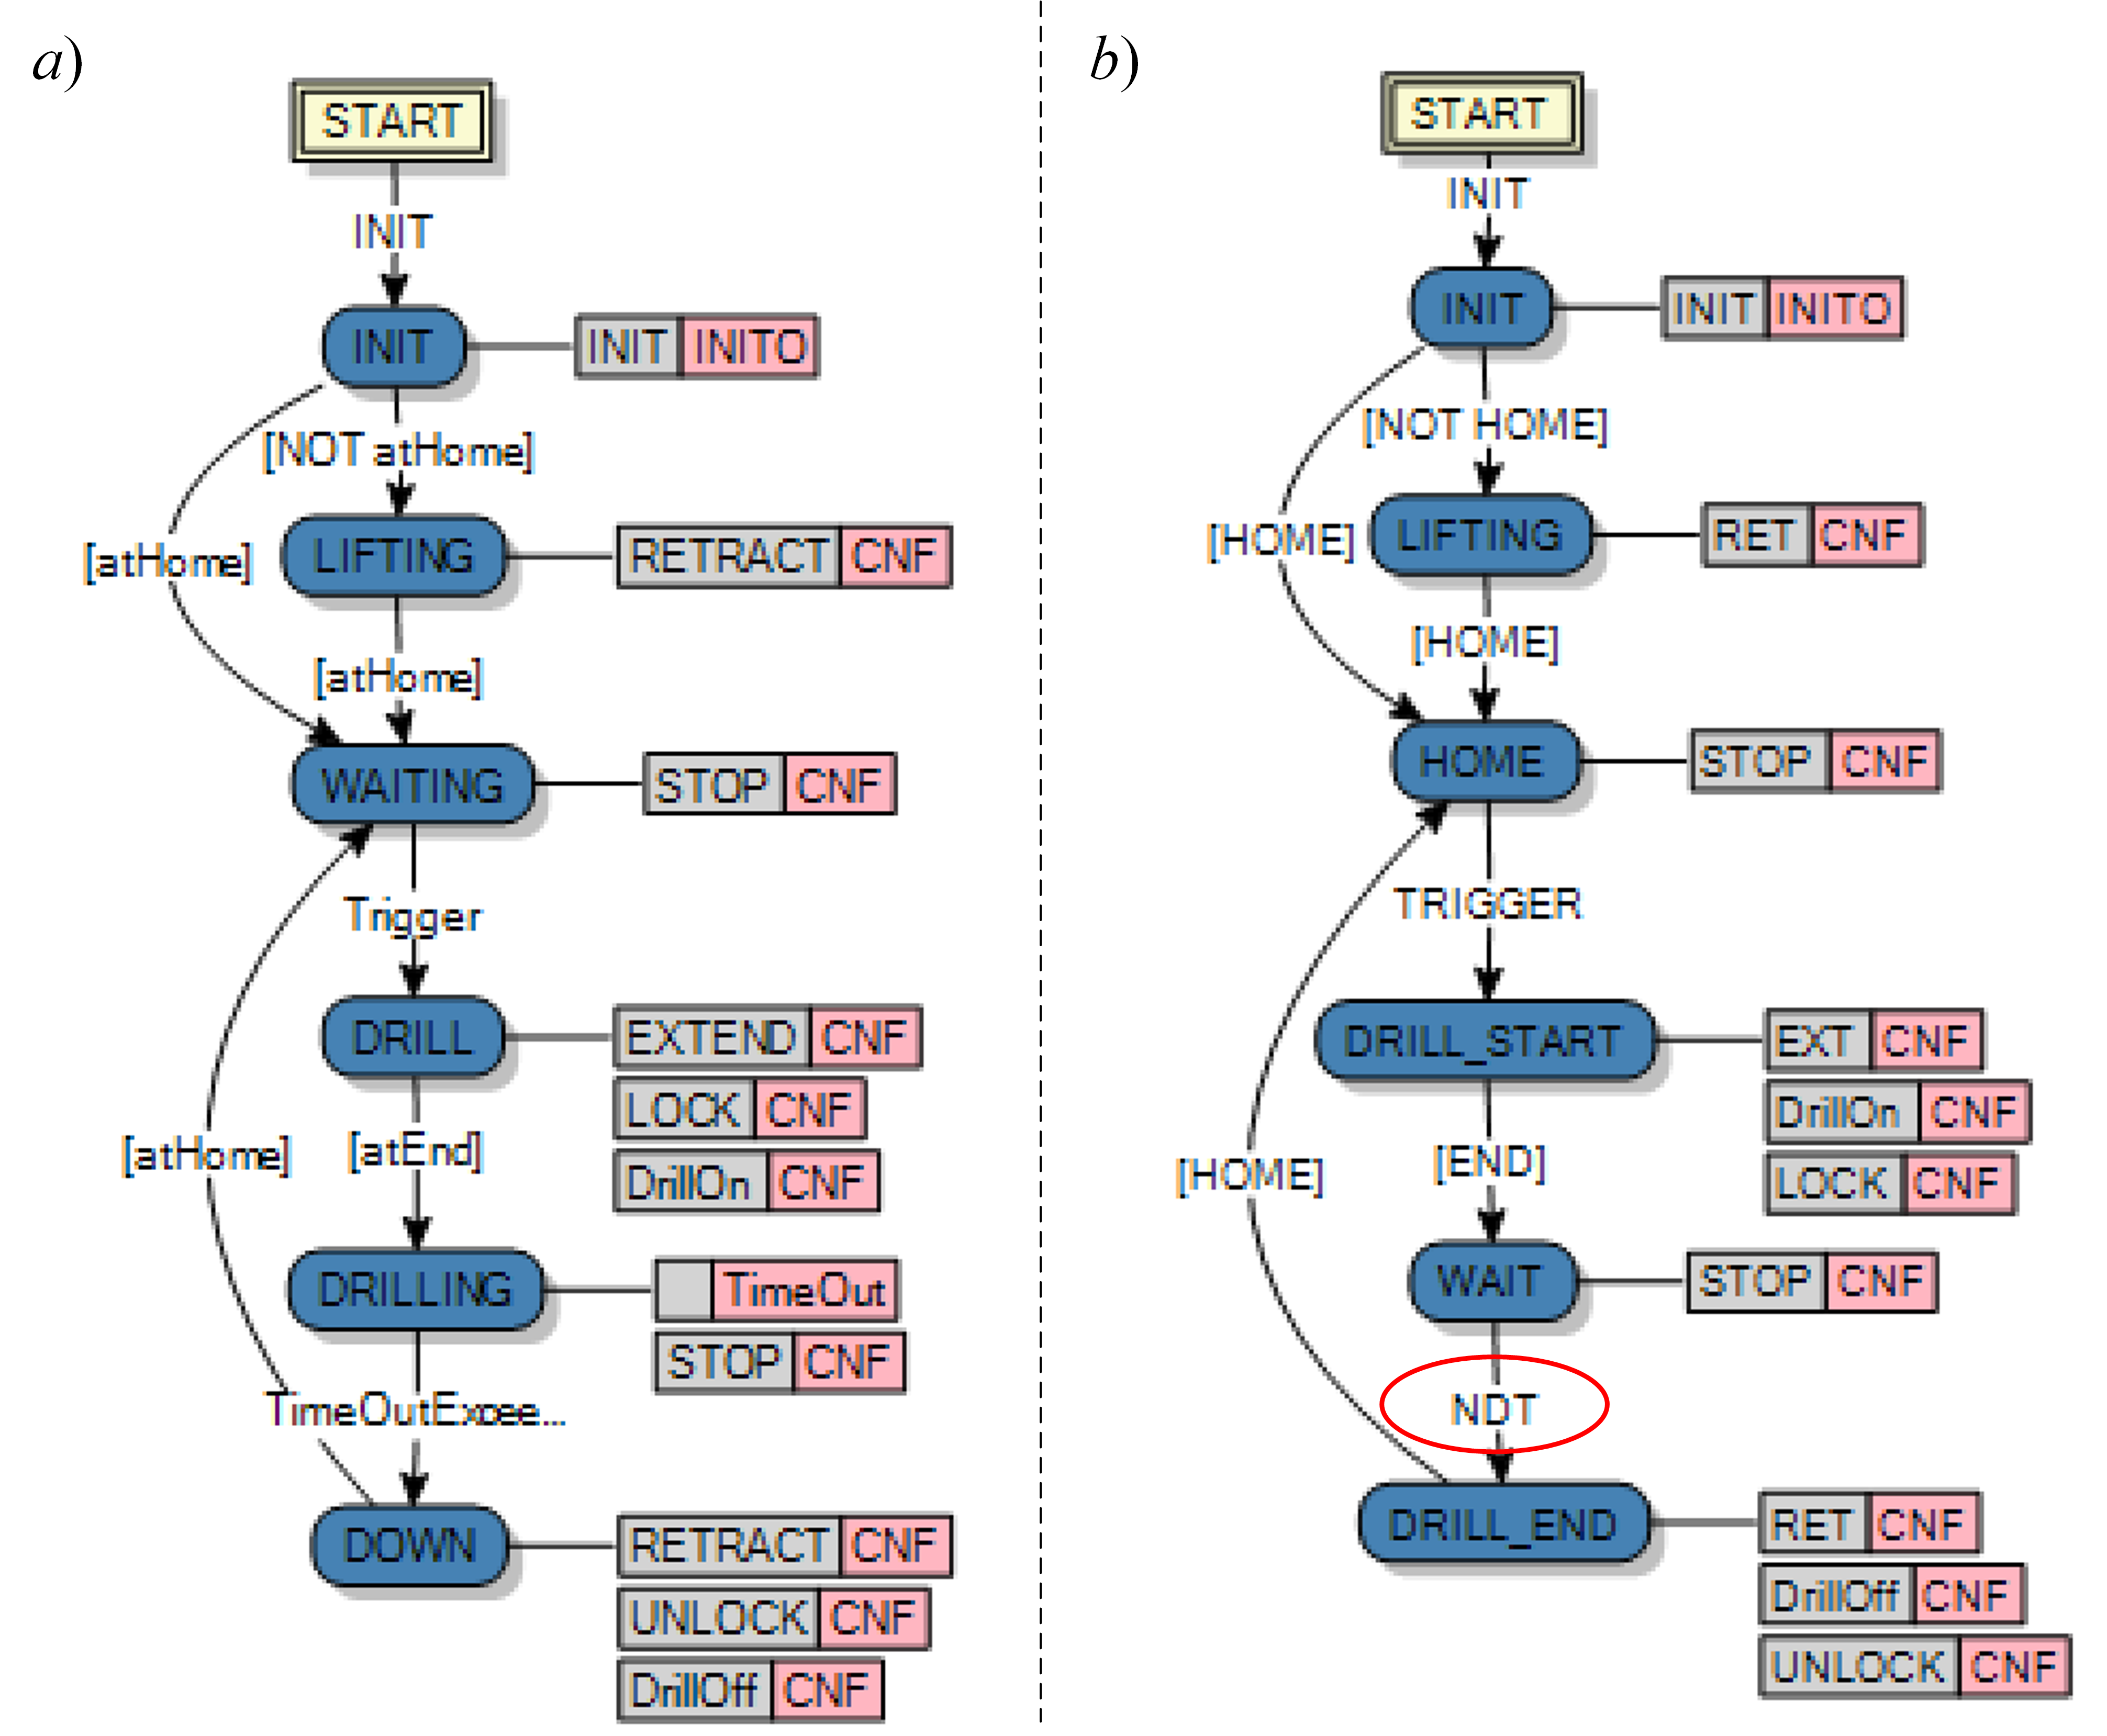
\includegraphics[scale = 0.24]{MX_Papers/Paper2/images/Fig10.png}
    \caption{ a) The ECC of the real drill controller; b) The ECC of the modified drill controller with a non-deterministic transition modelling the time delay.}
    \label{figure:DrillECCControllers}
\end{figure}


\subsection{Modelling of non-determinism in SMV}\label{sec:NDTinSMV}

%In some cases designers may assign incomplete value to the given signal to achieve the non-determinism in SMV to verify the specifications. 

%In order to attain the non-determinism in SMV, we need to provide the signal to choose different values in each transition. 

SMV provides a way to accomplish non-deterministic choice by providing a set of values to the signal. The first statement is used to  declare the variable NDT as a Boolean type and the second statement is used to initialize the NDT variable to either TRUE or FALSE value.

\begin{lstlisting}[breaklines,basicstyle=\small]
1 | VAR NDT:= boolean;
2 | init(NDT):= { TRUE, FALSE };
\end{lstlisting}
 In every  transition we are giving a provision to choose either TRUE or FALSE. This makes the NDT variable unpredictable in each transition.
\begin{lstlisting}[breaklines,basicstyle=\small]
3 | next(NDT):={ TRUE, FALSE };
\end{lstlisting}
Implementing non-determinism in every transition can be limited by introducing conditions in the next statement. If it is not required for the NDT variable to choose values in every transition then we can design like below:
\begin{lstlisting}[breaklines,basicstyle=\small]
4 | next(NDT):= case
5 | 	Condition: { TRUE, FALSE };
6 |     TRUE : NDT;
7 | Esac;

\end{lstlisting}

\section {{fb2smv} tool}
The {\bf fb2smv} tool \cite{fb2smv} is a model generator for generating SMV models of function block systems in IEC 61499. It is a part of formal verification tool-chain, that includes the model checker NuSMV and the tool for counterexample analysis in terms of the original FB system. 

The tool implements the formal model of IEC 61499 as per the modelling method present in  \cite{drozdov2021formal}. In order to construct {SMV} code, the {\bf fb2smv} tool uses Abstract State Machine (ASM) \cite{gurevich1995evolving} as an intermediate model. The tool takes  IEC 61499 function blocks expressed in XML format as input and generates a formal model with the help of ASM semantics. According to \cite{drozdov2021formal}, the structure of {SMV} code consists of  the declaration part and the rules part, which are the ASM rules.

%The paper describes  fb2smv tool \cite{drozdov2016formal} about the transformation rules based on execution semantics in detail.  

The tool converts basic and composite function blocks and also includes more additional features like, limiting the boundaries of variables to reduce the state space, changing execution order of FBs, deciding the input event priority by changing its order etc. The proposed non-deterministic transitions notation has been added to the tool as a result of this work. 

%The existing features of fb2smv and along with NDT functionality helps to create the accurate formal model. The fb2smv tool in the proposed tool chain makes the formal model creation of any CPSs in IEC 61499 standard easier.


\section{Results and Analysis}

In this paper, we demonstrated on a case study example, the use of IEC 61499 language for design and formal verification of cyber-physical automation systems. First, we designed the control logic of each mechatronic component in a drilling station and then implemented it as a function block in IEC 61499 standard. The simulation environment of the drilling station is developed with the help of the same controllers which are used in the real configuration. We reproduced the same plant behavior in the simulation model using the function blocks. In order to create a formal model of the system, we transformed existing function blocks of the plant models and controllers by adding non- deterministic transitions, using the proposed NDT notation. Using fb2smv  we converted the functional blocks to SMV code, which was verified using NuSMV on a machine with  Intel(R) core(TM) i7-10510U CPU @1.80GHz 2.30GHz  with 32GB RAM. The simulate feature of NuSMV was used to check the formal model's working behavior. Simulating the SMV code in interactive mode gives us the provision to go through each state by giving appropriate sensor inputs. We can try all possible input combinations to verify whether the system behaves as we expected. We can also randomly simulate the traces or we can manually go through each state by selecting different input combinations.

The main drawback of simulation is that the number of possible behaviors can be too large or even infinite. Simulation can show the presence of bugs, not their absence. 

More comprehensive verification can also be done by model-checking various properties, i.e. checking  whether a requirement  is true or not in all possible execution traces of control logic. This will allow us to test critical scenarios where there can be failures in some combination of inputs. The formal model of the system was verified with help of CTL \cite{emerson1985decision} specifications. While testing the CTL specifications in NuSMV, we found the following statement is false so it is possible that the table can rotate while the drilling process is going on.

\begin{lstlisting}[breaklines,basicstyle=\small]
-- specification  G !(DRILL_TABLE_CFB3_inst.DrillCTL_RET = TRUE & DRILL_TABLE_CFB3_inst.ActuatorGen_EO = TRUE)  
\end{lstlisting}

While executing the above specification, the NuSmv gave a counterexample that contradicts this statement. The counterexample generation for the above specification took 26000 seconds to complete. The counterexample helps to identify the error in the controller's design. We tested the same logic in the simulation model, the table rotated from its current position to another while drilling the workpiece. The real system also exhibits the same issue.

To fix this issue we need to analyze the counterexample provided by the NuSMV, but identifying the variables changed in each iteration is difficult. The Nutrac tool provides a better way to understand each state. The Nutrac tool converts the counterexample to a CSV file. This CSV file's columns represent states and rows represent input/output events or data input/output variables. We analyzed the CSV file and identified the issue. The issue was present in the execution control chart of the table's controller. It is required to add the BLOCK signal and it should be checked before moving from DRILLED state to REMOVED state. We verified the CTL specification again and this time NuSMV gave the TRUE result. The modified controller is tested in the real object, as well as in a simulation system and it was behaving as we expected i.e table was not able to rotate while drilling is going on.

In order to identify whether the  controller produces the {FWD} and {BACK} signals true at the same time, the following specification is used.

\begin{lstlisting}[breaklines,basicstyle=\small]
-- specification  G !(DRILL_TABLE_CFB3_inst.DRILL.Q_smv = ERROR_ecc)
\end{lstlisting}
 

After executing the above specification, the NuSMV produced the output as  TRUE.  The ECC of the drill model never goes to ERROR\_ecc state i.e. the controller never produces {FWD=TRUE} and {BACK=TRUE} condition simultaneously.  


This paper \cite{vyatkin2003verification} proposes  a software tool called VEDA (verification environment for distributed application), which is used for closed loop modelling and verification of distributed  control systems in intelligent manufacturing. Manually developed plants and automatically generated controllers are combined for model-based verification in IEC 61499 standard but it requires higher integration effort. The  paper \cite{Time-AwareComputations1} \cite{Time-AwareComputations2} describes a closed loop system with a simulation model used to autogenerate SMV but the resulting complexity was prohibitive. In this paper, we propose a methodology to create a closed-loop model staying within IEC 61499 standard which produces  lower complexity of model-checking than \cite{Time-AwareComputations1} \cite{Time-AwareComputations2} and reasonable engineering effort that is less than in \cite{vyatkin2003verification}.  

\section{Conclusion and Future Work}


In this paper, we proposed a tool chain which helps to verify and analyze the function blocks implemented in IEC 61499 standard.  This tool chain can be used for continuous development and evaluation of distributed control systems.  With the help of this tool chain,  it is possible to test the system quickly and efficiently. The accurate implementation formal model is necessary to identify all possible flaws in the system.  The existing functionalities of fb2smv along with the non-deterministic transitions in function blocks help to provide a similar formal model of the system.  Previously, the counterexample  analysis was complicated but now the Nutrac tool solves this issue by giving  a better representation of counterexample in CSV format. The developers working on complex system design can use this tool chain for continuous development and testing.


The non-deterministic transitions  in function blocks can be extended by introducing NDT as a variable to the FBs. This NDT variable can be any of any IEC 61499 data type but the NDT variable should be able to choose one value from set values.  For example, if we introduce NDT as a variable of integer data type and its values  limited 0 to 5 then it should be able to randomly select one value from 0 to 5.  In order to introduce more randomness to our formal model, it's better to implement NDT as a variable instead of using NDT as an event signal.  An interesting field to explore is if we can generate  the specification as well as the plant model automatically then existing manual interventions can be avoided. The tool chain which identifies all possible errors and fixes them automatically could be the next step in the future.

The models used in this paper are not based on time so the timing problems due to different set of time scales of controller and plant cannot be identified by this approach. The extension of notation to timed automata can be added for future work.

\section{Acknowledgements}
This work was sponsored, in part, by the H2020 project 1-SWARM co-funded by the European Commission (grant agreement: 871743).  

%%% Put references here
\putbib
\end{bibunit}

%-------------------------------------------------------------------
\def\paperheader{Paper C}
\def\papertitle{Formal verification of observers supervising a cyber-physical system implemented using IEC~61499}
\def\paperauthorstring{Polina Ovsiannikova, Etienne Le Priol, Vincent Perret, Pranay Jhunjhunwala, Midhun Xavier, and Valeriy Vyatkin}
\def\referencestring{Proceedings of the IEEE International Conference on Industrial Informatics (INDIN), 2021.}
\def\copyrightstring{2021, IEEE, Reprinted with permission.}

% The definitions above could just as well be put directly into the function
% call below, but were explicitly defined to more clearly illustrate the
% use of the function \makepaper.

\makepaperaccepted
  {\paperheader}
  {\papertitle}
  {\paperauthorstring}
  {\referencestring}
  {\copyrightstring}

% The actual contents is imported by un-commenting the \input line below.
% Make sure the file exist.
\begin{bibunit}
\thispagestyle{plain}

\section*{Abstract}
A rigorous check is a significant phase in the design process of control programs of safety-critical cyber-physical systems. Here, we consider such programs to be implemented using IEC~61499 standard for industrial automation. After the check is performed (for example, using formal verification), the engineer needs to ensure that even in unexpected situations, the system will not fail during the runtime, and for this online verification methods can be utilized.

In this work, we consider attaching monitors implemented as basic function blocks to the interface of the controller, thus having a property being monitored represented in the form of a state machine. Now, monitors make the system safer only if their quality is also ensured. Since their complexity is far lower than the complexity of the controller, they can be model checked, however, in the case of IEC~61499 function blocks, open-loop model checking will produce spurious counterexamples as it will allow combinations that are not possible according to the IEC~61499 function blocks semantics (e.g., data transferred without firing the event). The current work addresses this issue and proposes a method for close-loop model checking of monitors, using the non-deterministic twin of a controller under supervision. We present our approach using the system of two orthogonal pneumatic cylinders.

\section{\textsc{Introduction}}
%\PO{Continuing the topic of monitors in 61499 systems and their verification started in (Pranay, Monitoring design pattern for distributed automation systems in IEC 61499 and its formal modelling )}

%\PO{oflfine (static) verification of online (runtime) means for ensuring safety. }

%\PO{Works rarely cover testing of their observing mechanisms}

%\PO{There exist methods for monitoring IEC 61499 and methods for verifuinf IEC 61499, however there's none on verifying the monitors, which requires an interaction withthe system (?) }

%A rigorous check of safety-critical cyber-physical systems is crucial to industrial automation. 
Safety-critical cyber-physical systems must always comply with their requirements before they become operational. One of the important parts of the process of ensuring compliance is checking whether the control program (or controller) of such a system works as expected. This can be done using verification or validation approaches, which are united by the fact that none of them has a hundred percent coverage when dealing with complex industrial-sized systems. In the case of conventional testing or simulation, even if they are automated, some operational environment-related events might be left out and the industrial-sized system might be too complex to have all the possible test cases generated. Formal verification techniques allow the engineer to check the whole state space of the system; however, they suffer from a state-space explosion problem and of being computationally demanding overall when verifying complex systems. To combat this issue, various model abstraction techniques were developed to decrease model complexity (for example, to verify some particular functionality)~\cite{clarke2000,burch1992symbolic}. Another approach is bounded model checking, in which the executions of particular lengths are checked~\cite{biere2003bounded}. This, in turn, brings us back to the problem of missing a longer scenario that leads to failure.

Nevertheless, both approaches avail in finding the issues in the pre-operational stage, and what has to be added is an entity that would observe whether the particular property of the system holds during the runtime and communicate to an error handling system if the malfunction occurs. Such entities are called monitors or observers~\cite{17jhunjhunwala2022monitoring}. They can be internal or external to the system and perform the \emph{online verification}. Online verification has another advantage, i.e., if the changes have to be applied to the control program fast and there is a lack of resources to perform the global re-check, observers will maintain the safety state of the system by communicating the critical errors during the runtime.

In this work, our control programs are implemented following the IEC~61499 standard for industrial automation, and we consider internal monitors represented with basic function blocks, meaning that the properties of the system to be monitored are expressed as individual finite-state machines. This makes our monitors a better target for formal verification, and model checking, in particular, than the control program as a whole, since checking their whole state space requires less computational resources.

Model checking~\cite{clarke1999} is an approach for formal verification, where the formal model of the system is checked during the pre-operational stage, which is called \emph{offline verification}. In addition to a formal model of the system, model checking requires a formal representation of the properties of the system (for example, using linear temporal logic~(LTL)) as input. The model checker then derives all possible execution scenarios and produces counterexamples if the requirements do not hold. The counterexample for a requirement is such an execution scenario (or a system trace) where the requirement fails. 

Now, we propose to perform an offline verification (model checking) over the functional unit developed for online verification. Here, we face the issue that the traditional open-loop approach for model checking will produce spurious counterexamples due to the semantics of IEC~61499 function blocks~(FBs), where, for example, data cannot be sent or received without corresponding events being fired. 
We address this by modeling a non-deterministic twin of the controller and verifying a closed-loop model instead. We demonstrate our approach on a run-through example of two orthogonal pneumatic cylinders moving forward and backward. For model checking, we use NuSMV verifier~\cite{nusmv} and translate our FBs to its programming language (SMV) using the FB2SMV tool~\cite{drozdov2015fb2smv}.

The remainder of this paper is structured as follows. Section~\ref{sec:prelim} gives an overview of IEC~61499 standard and the verification methods of FBDs implemented according to it. Section~\ref{sec:method} describes a methodology for designing a supervised system, which is described in detail on a run-through example in Section~\ref{sec:methodappl}. Section~\ref{sec:concl} concludes the paper.

\section{\textsc{Preliminaries}}
\label{sec:prelim}
\subsection{IEC~61499}
IEC~61499 defines a design paradigm for distributed automation and control systems. The systems are implemented using the graphical language of function block diagrams~(FBDs). An FBD is a set of various interconnected FBs that can be of a basic, complex, or service interface type. In this work, we do not consider the latter. All FBs have their data and event input and output interfaces. The bricks of an FBD are basic FBs that represent atomic functional units. The logic of a basic FB is defined by an execution control chart~(ECC), which essentially is a Moore state machine and consists of states, transitions, and actions. In each state, an algorithm can be executed and/or an event (defined in the output interface of the FB) emitted. Complex FBs are nets of interconnected FBs of any type. The final FBD is assembled using the available FBs.

IEC~61499 systems are event-driven, unlike, for example, \mbox{IEC~61131-3}~\cite{tiegelkamp1995iec} systems that follow a cyclic execution pattern and \emph{event} is a key concept for the standard. Any event input or output can be bound to a subset of data inputs or outputs, respectively, which means that the corresponding data will be received and processed or sent only if the particular event fires. Intuitively, any update of the event variable opens the gates for the data connected to it.

In this paper, we create our observers using basic FBs, incorporating the logic of the condition to be monitored in their ECCs. As in~\cite{toolchain}, we use Non-Deterministic Transitions~(NDT) to create a non-deterministic twin of the controller of two pneumatic cylinders to verify the observers in a closed loop.



\subsection{IEC~61499 verification}
There exists a sufficient amount of literature on the topics of online (dynamic) and offline (static) verification of IEC~61499 FBDs. 

An overview of both static and dynamic verification approaches is given in~\cite{15blech2016comparison}.
\cite{12yoong2010verifying} proposes an approach of converting IEC~61499 FBs to Esterel and its subsequent verification.
In \cite{13yoong2015verification,14bhatti2011observer}, the monitors expressed as IEC~61499 FBs are added not for run-time verification but to better understand the counterexamples produced by the static verification approach. The system represented as a Kripke structure, together with observers and (possibly) computation tree logic~(CTL) formula are provided as input to the verification module. The authors suggest that, if the counterexample is received, the debugging process is simplified, as observers are inserted into the system structure.
\cite{11lindgren2016contract} considers static verification by enriching FBs with formal contracts and addressing verification on the component, algorithm, and ECC levels. In the works~\cite{agn_case_study} and~\cite{agnostic} the authors translate FBDs to SMV closed-loop formal models, \cite{toolchain} continues in this direction and presents a notation within IEC~61499 syntax for the subsequent generation of closed-loop formal models of FBDs and their verification by means of NuSMV. 


Examples of dynamic verification include, for example, \cite{1falcone2022runtime} that proposes adding enforcers to the application, which will not only monitor but adjust the supervised values in case of the property failure to ensure that the correct values are emitted by the controller. In~\cite{3do2020towards, 8ng2019contract}, the authors add assume and guarantee contracts in the form of FBs to the application to monitor the system during the run-time. \cite{4wenger15behavior} introduces behavioral runtime monitors into the 4DIAC framework. These monitors are generated automatically using service sequences extended with behavioral types. Combining various control and verification techniques, a reconfiguration architecture for fault handling in industrial systems is designed in~\cite{10leitao2020fault}. 


Approaches for dynamic and static verification, both, have their advantages and serve their purposes, hence, probably, the best way to ensure the system's correctness is to complement one with the other. However, despite the fact that there are numerous approaches for online verification, very few articles mention that the diagnosis units themselves must undergo a sanity check, which is especially important in relation to IEC~61499 FBs, where an occasional missing event in a transition condition can make a monitor erroneous. The point is outlined in~\cite{9wiesmayr2022supporting} and in~\cite{17jhunjhunwala2022monitoring} an approach to verify the monitors using Timed Net Condition-Event Systems was mentioned. We continue the work~\cite{17jhunjhunwala2022monitoring} and elaborate on the static verification of monitors expressed as IEC~61499 FBs and the challenges it brings. 
 
\begin{figure*}[htb]
    \centering
    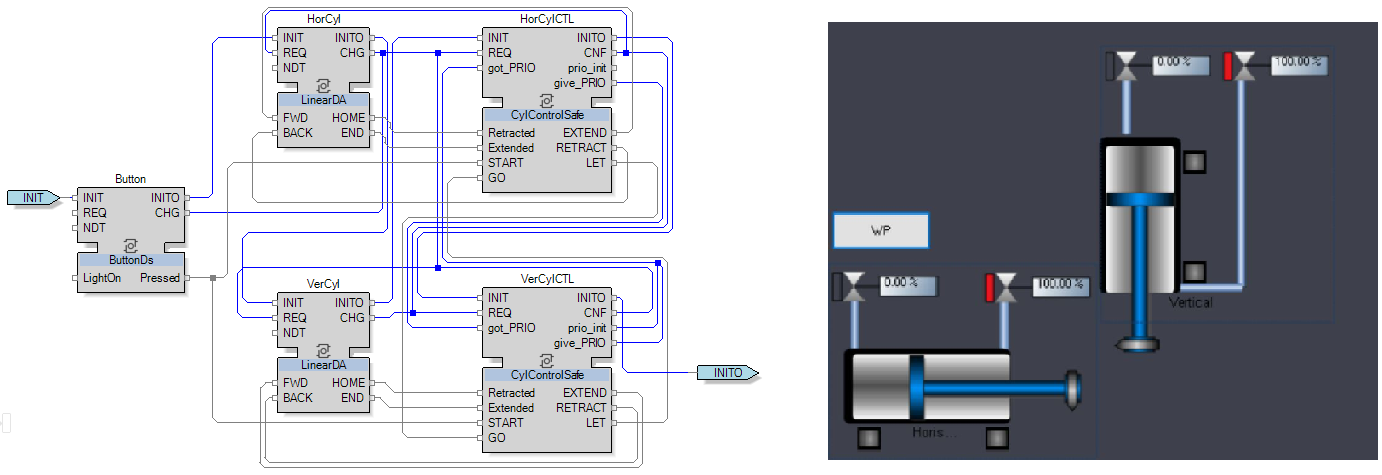
\includegraphics[width=0.98\textwidth]{MX_Papers/Paper3/pic/wholesystem_withhmi.png}
    \caption{The system of two pneumatic orthogonal cylinders. \texttt{HorCyl} and \texttt{VerCyl} simulate the plant (horizontal and vertical cylinder correspondingly), while \texttt{HorCylCTL} and \texttt{VerCylCTL} compose a control program. On the right, the HMI of the system is shown with the situation that should be avoided~-- a simultaneous extension of two cylinders.}
    \label{system}
\end{figure*}
%Tu t'es trompé de réseau de Pétri, le réseau où les deux cylindres ne se touchent pas c'est l'autre, tu l'as ou pas? 

\section{Design methodology for a monitored control program}
\label{sec:method}

For an automation system to function according to its specification, it must be checked using offline verification methods and equipped with online verification mechanisms to ensure that the requirements hold in unexpected circumstances. For this, the runtime verification means should also be checked.
Thus, in this paper, we propose a design methodology for the control programs implemented in form of IEC~61499 FBDs with internal observers (or monitors) that solves the aforementioned problem. Given a plant model (plant simulation program), for a single monitor, the methodology involves the following steps:
\begin{enumerate}
    \item Implementation of the control program.
    \item Verification of the control program in a closed loop with the plant model provided. Depending on its size, the plant model can be simplified and the heuristics for reducing the resulting closed-loop formal model state space may be applied. If the issues are found, the engineer has to address them and repeat this step until the verification result is positive.
    \item Formulation of a desired property to be observed in the form of a finite state machine and its implementation as a basic FB, i.e., implementation of the monitor.
    \item Implementation of the simplified non-deterministic twin of the controller that can produce any combination of outputs based on any combination of inputs. Verification of the created monitor in a closed loop with the twin. The properties to be formulated for the verification procedure, intuitively, are the following: the monitor indicates a failure when the failure occurs and the monitor does not report a failure when the controller functions as expected. If problems are found, they should be eliminated, and the system re-checked. This step should be repeated until the verification yields no counterexamples.
    \item Verification of the monitor in a closed loop together with the real control program.
    \item Verification of the monitor in a closed loop together with the control program where the fault was injected. Steps~5 and~6 may employ bounded model checking techniques or heuristics for state space reduction. The steps must be repeated if there were found issues to be addressed.
\end{enumerate}

The main contribution is concentrated in step~4.
In the next sections, we demonstrate our methodology step by step on a run-through example of a system of two pneumatic cylinders, especially focusing on step~4.


%As a base for our work, only one model is needed : an existing system. The first aim is to add a monitor to this model. The monitor added is not trustworthy, it has to be verified. 

%In order to avoid a kind of dependence to the current version of the system which needs to be checked, the monitor has to be verified independently. These formal verification have to ensure that the monitor would be able to output the correct result based on its inputs.\\
%In this paper, different kinds of formal verification of monitor will be approached. To prove and demonstrate that the method used is correct, we will use two systems with their behaviour verified. The first system is fully functional, while the second one is a dysfunctional analog of the first, with the error known. Those system are described in the Paragraph \ref{study_case}~~.

%For formal verification we used LTL expressions.

%The aim of this study is to reduce the number of checks of the entire system due to slight/little/minor modifications. Our idea is relies in the follows. Once the monitor is fully checked, it becomes trustworthy and able to check the behavior of the system instead of the formal verification.
%
%v2
%As a base for our work, only one model is needed: an existing system. The first aim is to add a monitor to this model. The monitor added is not trustworthy; it has to be verified. Different kinds of verification are needed to ensure that the monitor would work and would be able to verify our system. 
%The first verification considers the internal functioning of the monitor. A formal verification is applied to the monitor involving only its internal variables. The objective is to check the monitor's ability to output the correct result.
%The second verification is about its externals links. A second formal verification is applied to the monitor. This verification involves some of its internals variables and variable from the system. %pas clair
%The aim is to verify the functioning connections between the system and the monitor : its ability to correctly 'read' the working inputs.
%Once the monitor is fully checked, it is trustworthy and able to check the system's behaviour. This method allows us to avoid formal verification of entire systems and subsystems which would cost a significant amount of time especially for minor modifications.
%These formal verification are ensured thanks to LTL expressions.
%In this paper, to simplify the study at first, the system studied is a verified working system in order to ensure that mistakes only come from the monitor and not from the system. 
%To demonstrate the reliability of a formally verified monitor, this method will be applied a second time on the same system with behaviour modifications.
%The method described above will be applied a second time/once more with a dysfunctional system in order to prove the efficiency of the method. The dysfunctional system is the same model with voluntary dysfunctions that will be described in the following paragraph.
%
%v1
%As a base of our work, two models are needed : an existing model working as expected and the same existing model with voluntary dysfunctions. The first aim of adding same monitors to those models is to ensure that monitors work and are able to detect bugs that we have implemented. The systems are checked by Online verification.
%The second aim is to do formal verification of the models. LTL expressions have to contain variables from the working system and from the monitor. For the working model, the issue is to ensure that the monitor doesn't detect error which don't exist. For the dysfunctional model, LTL expression issue is to ensure that the monitor only detect errors. Once specification of LTL expressions are respected, it means that the formal verification from the system is the same as the formal verification of the monitor. The monitor is trustable.\\
%To confirm again the trustworthiness of monitors, systems studied here will be modified. The modifications applied do not have to change the main function of the system. Same process then will be applied to our modified system : multiple formal verifications with different LTL expressions. Finally, in the case of monitors and formal verifications outputting same 'things', it would proved the reliability of monitors checked with formal verification.
%This  verification is useful for more complex system. Offline verification is a real loss of time in the case of minor modifications. Limit of formal verification are not known thus this method implies to work with a simple model in order to avoid first endless calculations. 

\section {Methodology application}
\label{sec:methodappl}
\subsection{Steps 1 and 2: control program implementation and verification}

Our task was to create a control program for two orthogonal pneumatic cylinders that move towards each other and back by pressing a switch button. The plant simulation model was implemented as an IEC~61499 FBD in EcoStruxure Automation Expert (EAE).

The aim of the controller was to allow both cylinders to extend and retract once the button was pressed. The following safety requirement was to prevent the cylinders from colliding.
Thus, we implemented the priority system so that the horizontal cylinder can start moving only when the vertical cylinder is retracted. The complete system is presented in Figure~\ref{system}. Here, the control program consists of two controllers (for vertical and horizontal cylinders) of the same FB type that are connected in a closed loop with their plant models (cylinders). When the button is pressed, the command \texttt{START} is sent to the controllers and the cylinder with the higher priority gets the command to start its moving cycle (extend and retract). After the controller recognizes that its cylinder is retracted, it sends the priority giving event (\texttt{give\_PRIO}) to the vertical cylinder and sets the variable \texttt{LET} to true, allowing the vertical cylinder to take its turn.




%As it is stated in the Section~\ref{method}, there exist two versions of this system, i.e., correct and erroneous. Both of those systems are built using five Basic FBs. The first one is the controller(prev. switch?), once "pressed", it allows cylinders to move. Then, there are blocks that model the physical device of each cylinder (alternatively, we can call them plant blocks). They execute order of the command bloc such as "EXTEND", "RETRACT" or "STOP". Finally, there are command blocks of the horizontal cylinder and of the vertical cylinder. Those blocs receive information from the switch FB and send orders to the plant FB.
%The two cylinders are controlled and described the same way by the same FBs (same class but different objects).

%The most crucial requirement for our system is that the cylinders must never collide. Figure~\ref{system} shows the FB network of our correct system and its function is illustrated with a Petri net.\\
%Each cylinder has a priority, in our case, the priority of the vertical cylinder is higher than of the horizontal one. Therefore, when the button is pressed and both of variables \texttt{START} become \texttt{true}, the cylinder with a higher priority moves first. 
%In the end of its motion, the horizontal cylinder sends the priority giving event (\texttt{give\_PRIO}) to the vertical cylinder and sets the variable \texttt{LET} to true, allowing the vertical cylinder to take its turn.
%Thus, the system works in an infinite cycle. The system is forced in such a way that they cannot collide but neither are they able to extend a the same time no matter how many times the button is pressed.

In our case, the system is of a moderate size and we can apply model checking as is, without abstracting the system or using bounded model checking.
%To ensure that those models behave as expected, we model checked them using NuSMV verifier. 
Thus, we translated our system to SMV code using the FB2SMV tool and checked the following LTL formula with NuSMV verifier: \texttt{G $\neg$(Ver.EXTEND $\land$ Hor.EXTEND)} (where \texttt{Ver} and \texttt{Hor} are \texttt{VerCylCTL} and \texttt{HorCylCTL} correspondingly), 
%{\small$$G!(Ver.EXTEND=TRUE ~~\& ~~Hor.EXTEND=TRUE)$$}
which means that at every discrete time step, the two cylinders never get the command to extend simultaneously. The verification result was successful. 






%v1
%The method was implemented in the following case study: two perpendicular double-action cylinders commanded by a switch press button. The model is represented in Fig. 1. It is designed with IEC61499 standard through \textit{EcoStruxure Automation Expert (EAE)}.
%
%There are many different kinds of model of this system. First, we have the FB network which allows us to simulate with the HMI interface (Human Machine Interface) represented in Fig. \ref{petri_hmi_iec}(c). This model uses CAT FBs. CAT FBs are used to connect the Canvases objects in Fig. \ref{petri_hmi_iec}(b) and defined behaviours as forward and backward motion. They are plant FBs. However CAT FBs can not generate fbt files which are needed to do formal verification.
%Thus, we have a second FB network model allowing for a formal verification. CAT FBs are simply just substituted with basic FB also describing, thanks to ECCs, the forward and backward motion. These plant basic FBs' ECCs are built with NDT events which can be emitted at any time. It allows the formal verification to create many different combinations. \cite{toolchain} %of variables
%\\
%In both models, command of cylinders is controlled by basic FB. It is used to receive information from the switch press button and send information to the plant FB.
%The two cylinders are controlled and described by the same FBs (same class), with only objects being different.
%
%As said in the Method paragraph, we need two systems : the first one have to work perfectly and the other have to be dysfunctional. 
%The correct behaviour here is the case where cylinders never collide. Fig. \ref{petri_hmi_iec}(a) and \ref{petri_hmi_iec}(b) shows the FB network of our working system and it global operation illustrated with a Petri net.
%\\
%An order of priority has been defined upstream. During initialisation, the vertical cylinder gives priority to move to the horizontal cylinder. Once the switch button is pressed a 'START' signal is sent to the horizontal and to the vertical command FBs. To move, first, both cylinders need to have priority. Cylinder then will be in a waiting 'START' event state as it is shown in Fig. \ref{petri_hmi_iec}(b).

%Thus, the horizontal cylinder goes first. Just before the end of its motion, the command FB of the horizontal cylinder gives priority to the vertical cylinder letting it in the waiting 'START' event state and, at the end of its motion, sends a 'START' event: 'GO'\footnote{\label{GO}IEC 61499 rules does not allow two different outputs for a single data input. Another must therefore be created.} to the vertical cylinder, allowing it to move. 


%The system describes an infinite cycle where the horizontal cylinder moves first. Once the button is pressed it cannot be stopped. The system is forced in such a way that they cannot collide but neither are they able to extend a the same time no matter how many times the button is pressed.

%The dysfunctional system is different in terms of command FBs. There is no more priority rule. Once the switch button is pressed, the cylinders are both able to move at the same time and thus to collide as shown in Fig. \ref{petri_col}.
%both systems have
%The system has been checked firstly with HMI first and then with formal verification. Formal verification is described with the following LTL expression: 
%{\small$$G!(Ver.EXTEND=TRUE ~~\& ~~Hor.EXTEND=TRUE)$$}
%This means that for every combination of value of variables (G), the two cylinders never (!) extend at the same time. Expected behaviour has been observed, the LTL expression is always true in our assumed working system .
%and multiple counter-example have been found in our assumed dysfunctional system. 


\subsection{Step 3: Monitor implementation as a basic FB}


The next step was to create a monitor that would observe whether the safety property (i.e., two cylinders should never receive the command to extend simultaneously) is maintained by the system during the runtime. We implemented the monitor as a basic FB and assumed that it would be connected to the controllers as in Figure~\ref{fig:monitorplacement} (other connections are not depicted for the sake of clarity).

%The monitor has to observe the system the same way (as) the previous formal verification (did). This means that it has to check that the two cylinders never extend at the same time. 

\begin{figure}[h!]
    \centering
    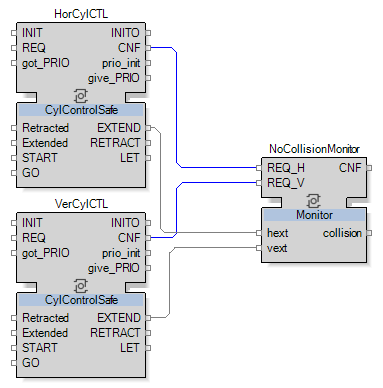
\includegraphics[width=0.35\textwidth]{MX_Papers/Paper3/pic/monitorplacement.png}
    \caption{Monitor \texttt{NoCollisionMonitor} connected to the controllers (other connections are not shown for clarity).}
    \label{fig:monitorplacement}
\end{figure}

%This monitor was implemented as a basic function block. 
The monitor receives the \texttt{EXTEND} outputs from both controllers together with their events \texttt{CNF} and communicates whether the collision is occurring by setting its output \texttt{collision} to \texttt{true} and triggering the \texttt{CNF} event. The ECC of the monitor is presented in Figure~\ref{fig:monitorecc}.

%Its ECC, Figure~\ref{ECC} is able to know (when and) which cylinder is extending. 'OBSERVER' FB only returns 'collision := TRUE' when the 'HextANDVext' state is reached.

%After multiple online tests with the functional systems, the monitor seems able to output a consistent result with our system behaviour.
%The monitor shown here can present mistakes, so it is susceptible to change depending on results of its formal verification.

\begin{figure}[h!]
    \centering
    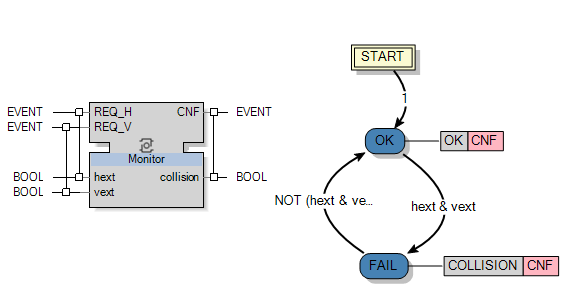
\includegraphics[width=0.48\textwidth]{MX_Papers/Paper3/pic/monitorecc.png}
    \caption{Interface of the monitor and its ECC. Algorithms \texttt{OK} and \texttt{COLLISION} set output variable \texttt{collision} to \texttt{false} and \texttt{true} correspondingly.}
    \label{fig:monitorecc}
\end{figure}

\subsection{Step 4: monitor verification with a non-deterministic twin of the controller }
\label{sec:monitorver}
The next step is to verify the implemented monitor in a closed loop with the controller (which we decompose into two controllers~-- for vertical and horizontal cylinders). In our case, the controllers are represented with basic FBs, and the closed-loop model checking will produce the result within an acceptable time interval. However, we will have to close the loop on the inputs of the controllers as well, meaning that we will either have to model simplified plants or provide other means for the controllers to produce all the possible combinations of their output values. Moreover, even if we succeed in closing the loop on the controllers, in case issues are found during the model checking, counterexamples will be hard to decipher as they will elongate and dozens of additional variables will be added to the system state.

Thus, we propose creating a \emph{non-deterministic twin} of the controller, which will be represented with two FBs of the same type just like our individual cylinder controllers. Now, let us disclose the notion of a non-deterministic twin~(ND twin). 

To model check the monitor, it is important that the model checker would infer all the possible combinations of its inputs, meanwhile triggering the events associated with them. Therefore, the goal of an ND twin is to abstract the logic of the controller by saving its key states, where the variables that are monitored change and add the non-deterministic transitions~(NDT) between them. Such events in an FBD turn into non-deterministic inputs in the SMV module of the corresponding FB, generated by FB2SMV as described in~\cite{agn_case_study}. 

The ECC of our individual controller of the cylinder together with its ND twin are presented in Figure~\ref{fig:ndtwinecc}. Two states that change the supervised variable \texttt{EXTEND} are \texttt{EXT}, \texttt{RETRACT}, and \texttt{STOP}. We kept them in the ND~twin and added NDTs between them so that at any time any output could be produced. From the algorithms, we remove everything that does not influence the variable \texttt{EXTEND} and leave only the \texttt{CNF} event associated with it. Figure~\ref{fig:ndtwinloop} shows two ND~twins of the controllers connected to our monitor.

\begin{figure}[t]
    \centering
    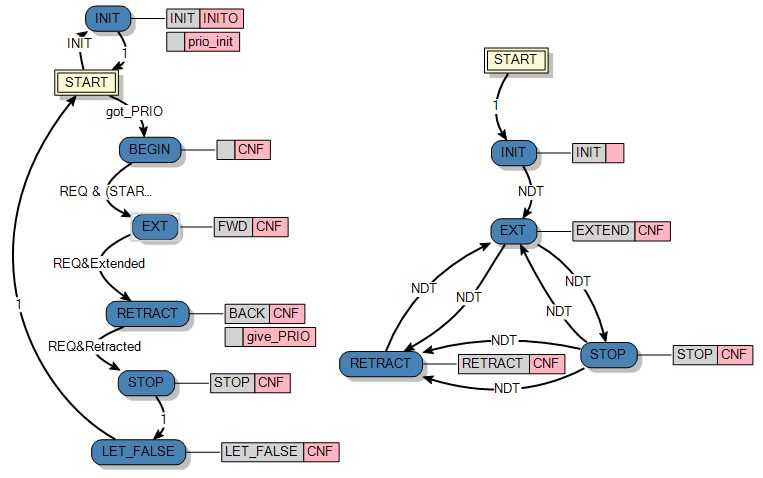
\includegraphics[width=0.5\textwidth]{MX_Papers/Paper3/pic/ndtcontrollereccs.png}
    \caption{ECCs of the cylinder controller (to the left) on of its ND~twin (to the right).}
    \label{fig:ndtwinecc}
\end{figure}


\begin{figure}[b]
    \centering
    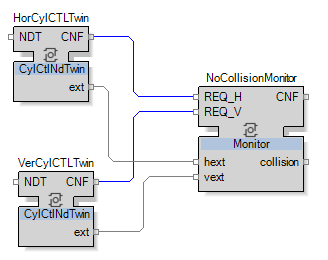
\includegraphics[width=0.34\textwidth]{MX_Papers/Paper3/pic/ndtwinloop.png}
    \caption{Connection of the monitor to ND~twins of the cylinder controllers.}
    \label{fig:ndtwinloop}
\end{figure}

When the system is converted to SMV, the first step is to verify that we can indeed get all the values of the monitor input, that is, our ND twins function according to their specifications. The set of properties that make up the specification can be created according to the following template. 

Assume that we have a set of all the supervised variables in a single ND~twin $U$.
$\forall u \in U, \exists D_u$, where $D_u$ is a domain of $u$. Then, $\forall u \in U, \exists V_u = \{(u,v) \:|\: v \in D_u\}$, where $V_u$ a set of all possible assignments of $u$. Now, a set of all the possible combinations of the variables values is $C = V_{u_1}\times\ldots\times V_{u_n}, n = |U|$. Having $C$, we can now formulate the CTL specifications to be checked as a set $S$:
$$S = \{\textbf{AG} \:\neg(\bigwedge_{p \in P} u(p) = v(p)) \:|\: P \in C\},$$
where $P$ a set of variable and value pairs, $u(p)$ returns the variable name of pair $p$ and $v(p)$ its value. Thus, if any of the specifications from $S$ are satisfied, it means that their corresponding combination cannot be generated by a formal model of an ND~twin.
Similarly, we check if the observer can get all the possible combinations of input values.

In our case, we checked the following specifications for the ND~twins (here, \emph{twin} is replaced with the corresponding names of the FBs for horizontal and vertical cylinders controllers twins): \texttt{AG twin.EXTEND} and \texttt{AG $\neg$twin.EXTEND},~-- and four specifications for the monitor of type \texttt{AG $\neg$(NoCollisionMonitor.hext $\land$ NoCollisionMonitor.vext)} (we omit others to save space). All the specifications failed, which means that all the combinations were possible in our model. 

Now, that we know that our model produces all the combinations of inputs, we can formulate the properties of the monitor to be checked. The first one tells that whenever the monitor gets the signals that both of the cylinders extend simultaneously, it produces the warning. Its LTL equivalent is: \texttt{\textbf{G} ((m.hext $\land$ m.vext) $\rightarrow$ (m.hext $\land$ m.vext \textbf{U} m.collision))}, where \texttt{m.} is short for \texttt{NoCollisionMonitor.}. Here we use operator \textbf{U}~-- ''until'' instead of \textbf{X} (''next'') or no temporal operator due to the specifics of the generated SMV model, where several model evaluations should occur to obtain the result of the FB output.

The second property tells that if the cylinders are not extending simultaneously, the collision is not reported, which is in LTL: \texttt{\textbf{G} ($\neg$(m.hext $\land$ m.vext) $\rightarrow$ \textbf{F} $\neg$ m.collision)}.

Both properties were satisfied by our monitor.

%A new solution has been provided in this paper. Formal verification of the monitor alone could not deal with connections and it is hard to understand how formal verification emits the different event and datas of the monitor. To meet the needs of it, a new system is created and modeled. This system would be a kind of a twin of the original system able to create every possible case. A first version is designed.\\

%\begin{figure}[h!]
%    \centering
%    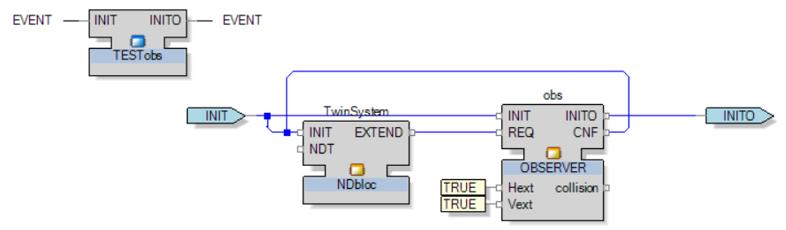
\includegraphics[width=0.48\textwidth]{MX_Papers/Paper3/pic/jumeau_V1.png}
%    \caption{First version of the twin two cylinders system}
%    \label{twin1}
%\end{figure}

%The twin system is composed of two FBs. The first one is the monitor and the other one is a simple basic FB able to output, thanks to a 'NDT' event, a 'EXTEND' event directly connected to the event 'REQ' of the monitor. moreover, datas of the monitor are forced as TRUE as seen in Figure~\ref{twin1}. Those 2 blocks are implemented in a composite FB and composed its FB network.\\
%During the formal verification, the event 'NDT' will be emitted randomly which will activate the 'REQ' event and thus the datas. LTL expression used here is the~(\ref{LTLmonitor}) one. A counterexample is found.

%As seen in the counterexample visualizer (Figure~\ref{vizu_twin1}), the monitor is still stuck in the 'OnlyH' state whereas Hext and Vext datas become TRUE at the same time. The twin system has to be improve but it already allows us to find some mistakes in the monitor. In facts, if the two datas become TRUE at the same time, in the ECC, it does not exist any transition for this case. Transitions are added. Then, if the system is stuck it's also because it can' read correctly transitions. The 'REQ' event is emitted once for two datas. It needs to be split into two different input events each will be link to one of the two datas. 'REQ\_h' is created and connected to 'Hext' and 'REQ\_v' is created and connected to 'Vext', Fig. \ref{monitorV2}.\\
%Now that two 'REQ' events have been created, a another bloc is added to the system in order to also trigger one of the 'REQ\_h/v ' event. A second version of the twin system is designed (Figure~\ref{twin2}).

%\begin{figure}[h!]
%    \centering
%    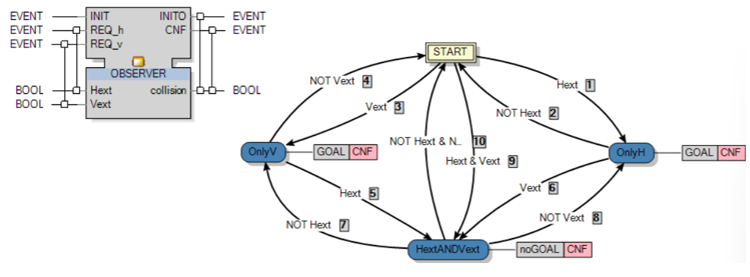
\includegraphics[width=0.48\textwidth]{MX_Papers/Paper3/pic/mointorV2.png}
%    \caption{Monitor and its ECC modified}
%    \label{monitorV2}
%\end{figure}

%A new formal verification is done, same LTL expression. Another counterexample, Figure~\ref{vizu_twin2}, is found. However, if watched more closely, the monitor is able to output that a collision happen but after few steps. Those few steps represent only steps needed to reach the good state and the time to activate the action allowing the monitor to output 'collision=TRUE'. The monitor here seems to work but to be more specific and make the formal verification founds no counterexample, the LTL expression needs to be modify. Using the function 'F', for future, would allows to reach our goal. The LTL expression now becomes :
%\begin{center}
%    $G(~(OBS.Hext = TRUE~~\&~~OBS.Vext = TRUE)$\\
%\end{center}
%\begin{equation}
%    \xrightarrow~~\textit{\textbf{F}}~~OBS.collision = TRUE)
%    \label{LTLmonitor2}
%\end{equation}


\subsection{Steps 5 and 6: monitor verification with the real and erroneous controller}

Now, we add the monitor to the system and check whether we connected it properly by verifying the system with the monitor as a whole. If the system at step~2 was checked using state-space reduction techniques, they can be applied here as well.

To check whether the monitor works when there is an error in the system, we inject the fault manually. In our case, we remove the priority mechanism from the controllers so that, by pressing the button, both cylinders extend simultaneously. The ECC of the erroneous cylinder controller is shown in Figure~\ref{fig:errctlecc}.

With both systems, we partially verify the same properties as in Section~\ref{sec:monitorver}. In both cases, we check whether all combinations of input values are possible for the monitor. The correct system reports that there is no possibility for two cylinders to get the extension command simultaneously, while only this is possible in the malfunctioned system. Then, we check the monitor properties, i.e., whether it reports the collision when it happens and does not report spurious collisions. Since the collision is not allowed in the first system, we omit the first monitor property, when checking the correct system, similarly, we omit the second property, checking the erroneous one. In both systems the checked properties hold, thus we can conclude that the monitor and its connections are correct.


\begin{figure}[t]
    \centering
    \includegraphics[width=0.34\textwidth]{MX_Papers/Paper3/pic/errctlecc.png}
    \caption{The ECC of the erroneous cylinder controller.}
    \label{fig:errctlecc}
\end{figure}

%Now it's to see if the monitor is still working while implemented in the correct model and the erroneous one. A new formal verification is made. No counterexample has been found in both model. The monitor is verified formally.




%The dysfunctional version of the described system is different in terms of command FBs. There is no more priority rule. Once the switch button is pressed, the cylinders are both able to move at the same time and thus to collide as shown in Figure~\ref{HMI_collide}.

%\begin{figure}[h!]
%    \centering
%    \includegraphics[scale=0.5]{MX_Papers/Paper3/pic/HMI_collide.png}
%    \caption{HMI representation of the two cylinders system colliding}
%    \label{HMI_collide}
%\end{figure}

%Monitor works online but there could be a transition path where a failure could appear. These paths can be determined with formal verification. The main aim of the monitor formal verification is to ensure that its internals are correctly designed. Misconceptions inside the monitor FB could be detected, i.e., an unreachable state.

%As said in the Section~\ref{method}, the monitor has to be checked independently from the system it has to observe. The first way to do it is to do the formal verification of the monitor alone. Indeed, from its own .fbt file, it is possible to do a formal verification. This formal verification would only involve internal inputs and outputs events and/or datas of the monitor ECC.\\
%The LTL expression has to verify the ability of the monitor to output the correct result depending on inputs. The LTL expression and its opposed should verify all the different cases.
%\begin{center}
%    \textit{G( (OBS.Hext = TRUE~~\&~~OBS.Vext = TRUE)}
%\end{center}
%\begin{equation}
%    \xrightarrow~~OBS.collision = TRUE)
%    \label{LTLmonitor}
%\end{equation}\\
%It means every time (G), if inputs \textit{Hext} and \textit{Vext} are true then the output \textit{collision} must be true.

%As a result, the LTL expression is always true, no counterexample has been found. This result allows to make a conclusion : the monitor works as expected.

%To see if it's true and if this kind of formal verification of monitors is enough to demonstrate that monitors are trustworthy, the monitor was added to both versions of the system (correct one and erroneous ones).\\
%When implemented in the functional system, checked with the same LTL expression~(\ref{LTLmonitor}), no counterexample is found. However, the system is functional so collision never happens. CHECK THIS It means that only the opposed of the LTL expression \ref{LTLmonitor} has been checked here, which is LTL expression~(\ref{LTLopposed}).
%\begin{center}
%    $G(OBS.collision = FALSE)$
%\end{center}
%\begin{equation}
%    ~~\xrightarrow~~(OBS.Hext = FALSE~~OR~~OBS.Vext = FALSE)
%    \label{LTLopposed}
%\end{equation}

%When implemented in the erroneous system, formal verification founds mistakes. Indeed, when the two cylinders are extending, the monitor is not able to output that there is a collision. Thanks to the counterexample of the visualizer, Figure~\ref{vizu_dys}, it is possible to understand what happen. Actually, the monitor is stuck in the 'OnlyH' state which outputs "no collision". Lots of hypothesis about the source of the problem but from now only a conclusion about this formal verification can be done: the formal verification of monitor only based on their .fbt file is not enough.



%The monitor works online but there could be a transition path where a failure could appear. These paths can be determined with formal verification.
%\\
%The main aim of the monitor verification is to ensure that its internals are correctly designed. Misconceptions inside the monitor FB could be detected by formal verification ie an unreachable state.
%
%In our case, the monitor FB is a basic FB so it is defined and composed by ECC.
%
%\subsubsection{Internal behaviour}
%First, only doing the formal verification of the monitor has been thought.\\
%This formal verification would only involve internal inputs and outputs events and/or datas of the monitor ECC and would be done directly from the \textit{fbt} file  of the monitor.
%\\
%The LTL expression has to verify the ability of the monitor to output the correct result. 
%LTL expression (ECC monitor alone)
%\begin{center}
%    {\footnotesize $G ((OBS.H\_ext = TRUE~~\&~~OBS.V\_ext = TRUE)$}\\
%    {\footnotesize$\xrightarrow~~OBS.collision = TRUE)$}
%\end{center}
%It means every time (G), inputs \textit{H\_ext} and \textit{V\_ext} are true then the output \textit{collision} must be true.
%\\
%As a result, the LTL expression is always true. It means that the ECC of the monitor works as expected.
%\\

%\subsection{Connections verification}
%However, the aim of a monitor is not to work alone, it has to be implemented. Moreover, the previous verification can not permit to conclude about the real behaviour of the monitor. In facts, to be fully checked, the monitor has to be simulated in a system which able to submit all the different possibilities of input combinations.
%
%A new system is created Fig. \ref{twin}. The aim is to recreate a simplified copy of the original system allowed to generate non deterministic events. Thanks to those non deterministic events and the NuSMV tool, the system will be able to generate all the different possibilities of input combinations.
%It composed of three basic FBs. One of them is the monitor. The two other FBs are twin of the cylinders command FBs. They are based on the same FB.
%\\
%As a basic FB, it is described by an ECC shown in Fig. \ref{ECC_twin}. Non deterministic events allows the state machine to evolve between its several states. The transition are called non deterministic transitions (NDT).
%\\
%When the \textit{'NDstate'}, for non deterministic state, is reached, the FB outputs the variable \textit{'EXTEND'} as true. Those outputs are directly connected to the observer bloc, one to \textit{'H\_ext'} and one to \textit{'V\_ext'}. The \textit{'EXTEND'} variable value is reset after that a second ND event (NDT2) is emitted.
%\\
%A quick online verification is made to ensure that the result is the same as the first online check in \textit{IV.B}.
%
%The system is verified offline with the following LTL expression :
%\begin{center}
%    {\footnotesize $G ((HorTwinCTL.EXTEND = TRUE~~\&~~VERTwinCTL.EXTEND = TRUE)$}
%    {\footnotesize$\xrightarrow~~F~~obsTEST.collision = TRUE)$}
%\end{center}
%
%This LTL means that every time (G) the \textit{'EXTENT'} variable of both basic FBs is true then the variable %\textit{'collision'} of the observer must be true instantly or in some states later (F).
%
%As a result, NuSMV finds counter-examples of this LTL expression. Which means that our monitor displays misconceptions.
%After being tested with all the different possibilities of inputs in a similar system, We thought our monitor could be considered as a certified working one.



%%%%%%%%%%%%%

%The monitor is 
%A first LTL expression has been test : 
%\begin{center}
%     {\footnotesize $G ((HorCTL.EXTEND=TRUE~~\&~~VerCTL.EXTEND=TRUE)
%     \xrightarrow ~~  (obs.collision=TRUE))$}
%\end{center} 
%But it return counters example. In fact, this LTL expression pretends that the detection of the monitor is instantaneous. In the detail of counter-example file, it is because the monitor detects the error several state after the two cylinders extend(ed/ing) at the same time. Therefore, we tried another approach :
%\begin{center}
%    {\footnotesize $G ((HorCTL.EXTEND=TRUE~~\&~~VerCTL.EXTEND=TRUE)
%     \xrightarrow~~$}
%     {\small $F(obs.collision=TRUE))$}
%\end{center}

%It means that the detection will arrive in the future (F) or, in other words, several states after the both EXTEND signals (verical and horizontal) came true . The potential drawback is that the detection arrive too late, but this can't be quantify in this case. Nevertheless, it is a starting point to avoid the previous issue. After implement this formula in Nusmv, it return that the LTL statement is TRUE.  

%%%%%%%%%%%%%%%%



%\subsection{Monitor implemented in the working system}
%\vspace{0.2cm}
%Now, the aim is to ensure that the monitor is correctly implemented in the system. The formal verification permits to test the connections of the monitor with the system. 
%\\
%The verification condition of our system is simple so are the connections between the system and the monitor. As said in the section \textit{B. Adding monitor} from the paragraph \textit{IV. STUDY CASE}, the monitor only reclaims two outputs from the command FB of each cylinder. A simple connections is needed (fig. \ref{monitor}). With the same LTL expression schema, this condition is checked.
%
%LTL expression (system+monitor in S)
%\begin{center}
%     {\footnotesize $G ((HorCTL.EXTEND=TRUE~~\&~~VerCTL.EXTEND=TRUE)
%     \xrightarrow ~~  F (obs.collision=TRUE))$}
%\end{center} 
%
%
%explanation of the expression
%This expression means : "IF the horizontal cylinder is extending AND (\&) if the vertical cylinder is also extending THEN ($\rightarrow$) the monitor must always (G) return "collision=TRUE". 
%\\
%It return that this LTL expression is always true.
%
%However, the system known as a working system, the variable 'EXTEND' of both cylinder can not be TRUE at the same time. Thus the LTL expression is not directly verified, only is its contraposition :
%\begin{center}
%    {\footnotesize $G(obs.collision=FALSE) \rightarrow~~$}\\ 
%    {\footnotesize $!~(HorCTL.EXTEND=TRUE~~\&~~VerCTL.EXTEND=TRUE)$}
%\end{center}
%
%\begin{figure}[h!]
%    \centering
%    \includegraphics[width=0.45\textwidth]{MX_Papers/Paper3/pic/IEC_syst_col.JPG}
%    \caption{IEC model design of the two cylinders able to collide}
%    \label{IEC_collide}
%\end{figure}

%\subsection{Monitoring with modifying the system} 
%\vspace{0.2cm}
%ajouter une transition pour dire que ca marche avec un system modifié en tout cas inchallah
%
%Now that monitor ECC is working and connections with the system are correctly established, our monitor is trustworthiness and able to fully diagnose online systems errors. To prove it, let's implement our monitor in a slightly different system.   
%\\
%The previous part assure that the monitor does not detect false error. However, we don't know is behaviour when it's linked to a system which include misconceptions.   
%
%Thus, we introduced a different system.
%it's actually the same as previously but with behaviour modifications.
%
%idée d'Etienne : il vient pas de poitier, permettre au système d'ateindre tout les états possible (ie même ceux "interdits") 
%
%Il n'a pas detecté d'erreur inexistante mais on ne l'a pas confronté à un système pouvant comporter des erreurs. Certe, ses entrèes sont cohérentes avec ses sorties (cf première LTL) mais (sinon on a juste à s'arréter à la vérif du ECC tout seul)) pas ouf 
%
%Nous avons vérifié les connections avec un système qui marche, nous avons vu que ces connections ne créent pas de fausses erreurs mais permettent-elles d'en detecter? c'est ce que nous allons voir en l'ajoutant à un système comportant des erreurs.
%
%
%
%%It is different in terms of command FBs. There is no more priority rule. Once the switch button is pressed, the cylinders are both able to move or not at the same time and thus to collide. As seen in Fig. \ref{IEC_collide}, the model design is almost the same and Fig. \ref{petri_collide} represented its Petri net.
%\\
%\begin{figure}[h!]
%    \centering
%    \includegraphics[width=0.3\textwidth]{MX_Papers/Paper3/pic/systeme_col.JPG}
%    \caption{Petri net  model of the two cylinders able to collide}
%    \label{petri_collide}
%\end{figure}
%
%% implementation of the monitor and online verification of the system
%The monitor is implemented in this system. It is connected the same way as it was in the previous %system : the monitor reclaims the 'EXTEND' variable from the horizontal and the vertical %cylinders (Fig. \ref{monitor} and Fig. \ref{IEC_collide}).
%%The monitor and its connections with the system, identically as before,  does not need any %formal verification. Pas compris
%
%Online verification may be run with the modified system. The monitor finds out that, at some %point, the two cylinders are extending at the same time. 
%\\
%If it sticks to the method plan, mistakes should come from the system - the monitor tells the %truth. To confirm this hypothesis, the system and the system with the monitor have to be %checked thanks to formal verification.
%
%FV of the system but no HMI verification just offline
%The system has been first checked alone - including only variables from the system. Formal %verification is described with the same LTL expression as the first system :
%{\small$$G!(Ver.EXTEND=TRUE ~~\& ~~Hor.EXTEND=TRUE)$$}
%
%Expected behaviour has been observed, the LTL expression is false, a counter-example file have %been returned with the expected mistake.
%\\
%
%Online, with adding the monitor, it can detect the simultaneous extend.
%\\
%However, when the monitor was added to the formal verification with the following LTL %expression : (the same as the working system)
%
%\begin{center}
%     {\footnotesize $G ((HorCTL.EXTEND=TRUE~~\&~~VerCTL.EXTEND=TRUE)
%     \xrightarrow ~~  F (obs.collision=TRUE))$}
%\end{center} 
%
%Then, NuSMV return a counter-example, not as expected. Therefore, our simplified system with all the possibility as to be reconsidered.

\section{Conclusion and future work}
\label{sec:concl}

In this paper, we presented a design methodology for the supervised system implemented in form of IEC~61499 FBD, putting special attention to the verification of the supervision mechanisms, that is, the monitors. This methodology allows using formal verification with state-space reduction or abstraction techniques while verifying the system as a whole, while creating reliable means for online observation of its function. Our main contribution is the approach for extensive closed-loop verification of monitors implemented in form of IEC~61499 FBs using the simplified non-deterministic twins of the controllers.

Having the system monitored gives an additional advantage while introducing small changes to the system when, for instance, the time does not permit performing the whole recheck. If the connections to the monitor do not change, with the proper setting of an error handling unit, the system will stay safe even if the new change leads to a failure.

The manual implementation of the proposed methodology may seem to cost time and effort; however, the process can be automated. Our future work in this direction focuses on creating the plugin to an open-source IDE for IEC~61499 programs, FBME~\cite{fbme}, that would implement the algorithm that distinguishes the key states of the controller, which change the variables under supervision, and generate a FB with NDTs between such states (i.e, ND~twin). The properties that should be checked on an SMV model of an ND~twin can also be generated automatically following the definition that we used in the current work. Thus, if we assume such a plugin, the input data for it would be a monitor, a supervised controller, and a set of temporal properties with which the monitor should comply. The subsequent check of the monitor injected into the system as a whole can be done semi-automatically, depending on the size of the SMV model of the system. 


Another direction of future work is to explore the scalability of our monitor-checking approach and verify more complex properties that include not only inputs of the monitors but any variable in the system, as well as monitors and controllers implemented as composite FBs.

%In our case, formal verification of the twin system is from 5.000 to 10.000 times faster than the formal verification of the entire system
\section*{Acknowledgments}
%\PO{This work was supported?} 

This work was supported, in part, by the HORIZON 2020 project 1-SWARM funded by the European Commission (grant agreement: 871743) and Horizon Europe project Zero-SWARM funded by the European Commission (grant agreement: 101057083).

We also wish to thank Dr. Igor Buzhinsky for suggesting us the missing piece of the puzzle during the work on Section~\ref{sec:monitorver}.

\putbib
\end{bibunit}





\printglossary[type=\acronymtype]

\end{document}
